\documentclass[titlepage]{article}
\usepackage[utf8]{inputenc}
\usepackage[italian]{babel}
\usepackage{graphicx} % Required for inserting images

% dimensioni foglio
\usepackage{geometry}
\geometry{a4paper, top=4.5cm, bottom=4.5cm, left=4cm, right=4cm} % heightrounded, bindingoffset=5mm}

\usepackage{enumitem}

% lista a diamante sempre
\setlist[itemize]{label=$\diamond$}

\usepackage[pdftitle = {sistemi-operativi}, pdfauthor = {imAlessas}, pdfdisplaydoctitle]{hyperref}
\usepackage{todonotes}
\usepackage{comment}
\usepackage{blindtext} % lorem ipsum
\usepackage{amsmath} % equation
\usepackage{listings} % estratti di codice
\usepackage{color} % colori
\usepackage{pxfonts} % bold keywords
% \usepackage{xurl} % vai a capo con url
\usepackage{tabularx} % fixed columns
% \usepackage{pdfpages} % incollare un pdf
% \urlstyle{same} % l'url ha lo stesso font del testo
% \usepackage{enumerate} % numeri romani nell'elenco
% \usepackage{longtable}
% \usepackage[autostyle]{csquotes}
\usepackage{wrapfig} % wrappo la figura sul testo

% indice delle immagini
\usepackage{array}
\graphicspath{ {figures/} }


% cambia da "Listing 1" a "Codice 1"
\addto\captionsitalian{%
\renewcommand{\lstlistingname}{Codice}}

% Cambia da "Listings" a "Elenco dei codici"
\addto\captionsitalian{% 
\renewcommand{\lstlistlistingname}{Elenco dei codici}}

\usepackage{tikz}
\tikzset{
  treenode/.style = {shape=rectangle, rounded corners,
                     draw, align=center, 
                     top color=white, bottom color=blue!30},
  root/.style     = {treenode, font=\normalsize, bottom color=grey!50},
  env/.style      = {treenode, font=\small},
}

%C++
\definecolor{lightgrey}{RGB}{250, 250, 250}
\definecolor{bordeaux}{RGB}{186, 0, 0}
\definecolor{turquoise}{RGB}{22, 161, 147}
\definecolor{grey}{RGB}{175, 175, 175}
\definecolor{green}{RGB}{0, 120, 0}
\definecolor{blue}{RGB}{0,0,255}
\definecolor{lightyellow}{RGB}{255,255,245}

% \lstloadlanguages{c} 
\lstdefinestyle{c++}{language=c++,
  % sfondo
  backgroundcolor=\color{lightyellow},
  % normale
  basicstyle=\ttfamily, 
  % parole chiave
  keywordstyle=\bfseries\color{blue},
  % commenti
  commentstyle=\itshape\small\color{bordeaux},
  % stringhe
  stringstyle=\color{green},
  % numeri a lato
  numberstyle=\tiny\color{grey},
  % 
  belowskip=3mm,
  breakatwhitespace=true,
  breaklines=true,
  classoffset=0,
  columns=flexible,
  framexleftmargin=0.25em,
  frameshape={}{y}{}{}, %To remove to vertical lines on left, set `frameshape={}{}{}{}`
  numbers=left, %If you want line numbers, set `numbers=left`
  showstringspaces=false,
  tabsize=3,
  xleftmargin = 1.5em,
  morekeywords = {nullptr, cout, cin}
}



\title{\textbf{\fontsize{35pt}{35pt}\selectfont Sistemi\\\vspace{25pt}Operativi}}
\author{Alessandro Trigolo}
\date{\today}

\begin{document}


\maketitle

\newpage\tableofcontents

\newpage\listoffigures

\newpage\lstlistoflistings


\lstset{style = C++}

\newpage\part{Gestione dei Processi}

\chapter{Processi}\label{processes}
Iniziamo dalle basi. Un \textbf{processo} è un programma in esecuzione, è un'istanza del programma che viene eseguita sulla CPU. Possiamo infatti avere diverse istanze dello stesso programma, ognuna che viene eseguita indipendentemente dall'altra. Possiamo quindi dire che il programma, ovvero il file eseguibile (\texttt{.exe}) è qualcosa di passivo mentre il processo è qualcosa di \textbf{attivo}.

% 
\section{Allocazione in memoria}
Andando un po' più in dettaglio, quando il programma è in esecuzione, questo viene eseguito in maniera sequenziale. Al processo, una volta che è eseguito, viene dedicato dello spazio in memoria dal sistema operativo. Come è possibile osservare nella figura \ref{fig:memory_layout}, la memoria messa a disposizione dal sistema operativo è suddivisa in diverse zone, ciascuna con un particolare compito.
\begin{figure}[h]
    \centering
    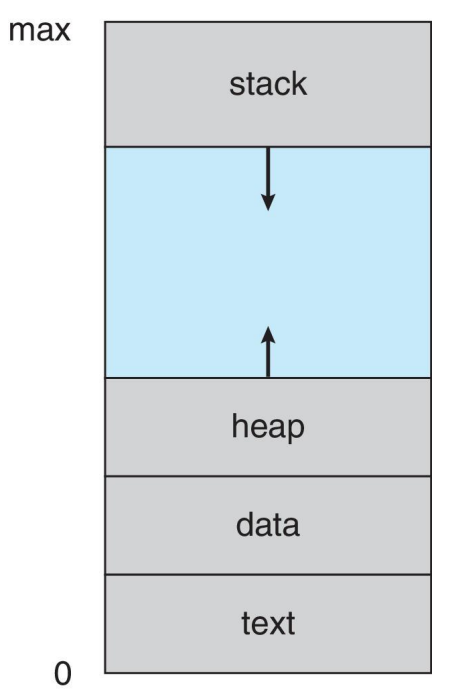
\includegraphics[width = .2\textwidth]{../res/imgs/processes/memory_layout.png}
    \caption{Spazio in memoria allocato per il processo dal sistema operativo.}
    \label{fig:memory_layout}
\end{figure}
Prima di tutto, il codice sorgente del programma viene caricato nella zona \textbf{text}. Dopo di che, nella parte dedicata ai dati (\textbf{data}) vengono salvate generalmente le variabili globali, che permangono per tutta la vita del processo. Sono infine presenti due parti: lo \textbf{stack} e l'\textbf{heap} che crescono in direzione opposta. Lo stack contiene dati temporanei come variabili locali mentre l'heap è utilizzato al fine di allocare la memoria dinamicamente durante la vita del programma\footnote{Come abbiamo visto con C++, heap e \textit{freestore} sono quasi dei sinonimi.}.

% 
\subsection{Process Control Block (PCB)}\label{PCB}
Ad ogni processo che è mandato in esecuzione è assegnata una particolare struttura dati dal sistema operativo, ovvero il \textit{Process Control Block} (figura \ref{fig:PCB}). Il PCB contiene diverse informazioni riguardanti il processo, in particolare:
\vspace{-5px}
\begin{enumerate}
\setlength{\itemsep}{-.15 em}
    \item Lo \textbf{stato} del processo;
    \item Informazioni sul \textbf{program counter}, in particolare è importante sapere se il processo è fermato temporaneamente e poi fatto ripartire più tardi;
    \item Valori dei registri, utili nel caso in cui un processo venga messo in pausa;
    \item Altre informazione riguardanti lo scheduling della CPU (vedi capitolo \ref{CPU scheduling}), come la priorità del processo;
    \item Informazioni per la gestione della memoria e dell'I/O.
\end{enumerate}
\begin{figure}[h]
    \centering
    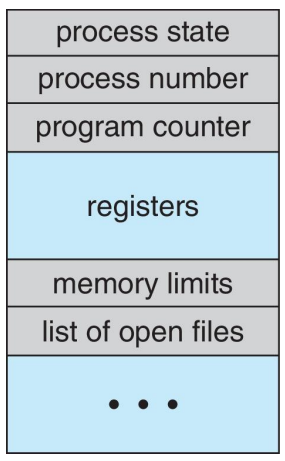
\includegraphics[width = .20\textwidth]{../res/imgs/processes/PCB.png}
    \caption{Rappresentazione del contenuto di un generico PCB.}
    \label{fig:PCB}
\end{figure}

\noindent In particolare, in \texttt{Linux}, nel PCB di un processo (che in Linux è chiamato \texttt{task}) sono presenti le seguenti informazioni: \texttt{pid} (numero assegnato al particolare processo), puntatori al processo genitore (che vedremo saranno utili nella fase di creazione di un processo), puntatori ai processi figli e altre informazioni come la lista dei file aperti. Quando un nuovo processo è creato in Linux, le sue informazioni sono detenute in una lista concatenata (\textit{doubly-linked list}) dove ogni nodo della lista è il PCB di un processo specifico (figura \ref{fig:process_table}). 
\begin{figure}[h]
    \centering
    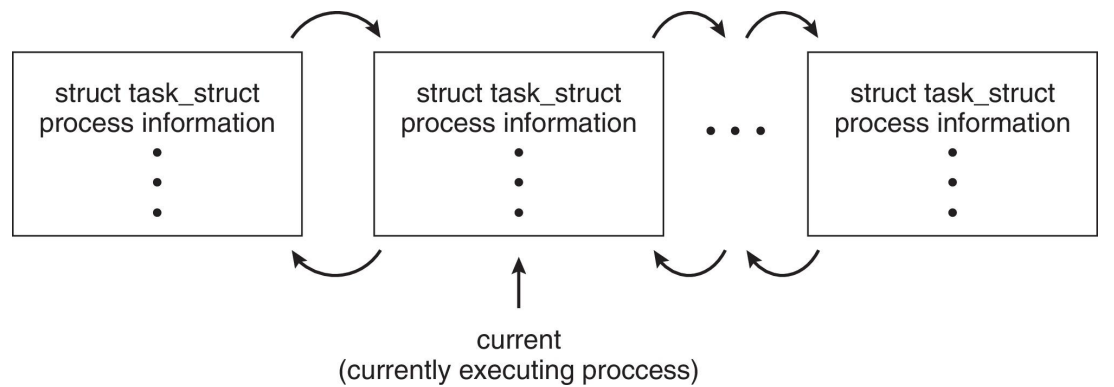
\includegraphics[width = .75\textwidth]{../res/imgs/processes/process_table.png}
    \caption{Lista concatenata che mantiene tutti i PCB dei processi (task) in Linux.}
    \label{fig:process_table}
\end{figure}
Al fine di andare a modificare delle informazioni del processo (come lo stato corrente) il sistema operativo scorre la lista e, dopo aver selezionato il PCB del processo desiderato, andrà a modificare il campo. 

% 
\section{Stati di un processo}
Durante l'intera vita del processo, questo passa in diversi stati (figura \ref{fig:process_life}). I principali sono:
\vspace{-5px}
\begin{enumerate}
\setlength{\itemsep}{-.15 em}
    \item \textbf{New}: il processo è appena stato creato;
    \item  \textbf{Ready}: il processo è pronto per essere eseguito, quindi non è ancora stato assegnato al processore e sta aspettando l'assegnazione;
    \item \textbf{Running}: dopo essere stato associato alla CPU il processo inizia ad essere eseguito. Come vedremo nel capitolo \ref{CPU scheduling} e successivi, il processo può essere interrotto e quindi ritorna allo stato ready;
    \item \textbf{Waiting}: se il processo deve aspettare qualche input da esterno si mette in attesa e una volta che riceve l'input ritorno nello stato ready;
    \item \textbf{Terminated}: una volta che il processo finisce la sua esecuzione, questo ovviamente termina e viene rimosso dalla CPU.
\end{enumerate}
\begin{figure}[h]
    \centering
    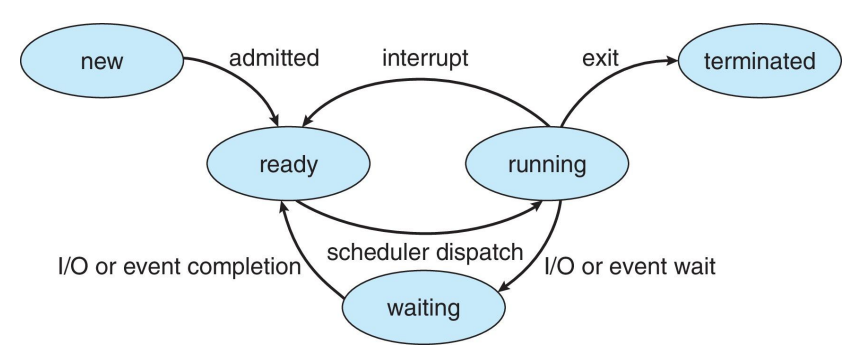
\includegraphics[width = .75\textwidth]{../res/imgs/processes/process_life.png}
    \caption{Gli stati della vita di un processo.}
    \label{fig:process_life}
\end{figure}

\noindent Lo stato \textit{ready} e lo stato \textit{wait} contengono delle code dove i processi attendono di essere eseguiti ovvero la \textbf{ready queue} e la \textbf{wait queue} che non sono altro che delle liste concatenate. Le liste contengono i PCB dei processi: il sistema operativo tiene traccia del primo e dell'ultimo processo nella lista al fine di riuscire a implementare le due code.  Possiamo inoltre suddividere i processi in due macro categorie:
\vspace{-5px}
\begin{itemize}
\setlength{\itemsep}{-.15 em}
    \item \textbf{CPU bound} che sono i processi che hanno un uso massiccio della CPU;
    \item \textbf{I/O bound}, ovvero processi che spendono la maggior parte del loro tempo in una situazione di wait per leggere o scrivere sulle periferiche.
\end{itemize}

% 
\subsection{Context switch}\label{context_switch}
Quando un processo A viene un rimosso dalla CPU, nel caso in cui sia stato interrotto per far spazio ad un altro processo B, è necessario salvare l'informazione del processo A in modo tale da poterlo sostituire con il processo B per poi, in un secondo momento, riuscire a ricaricare il processo A. Questa operazione è  detta \textbf{context switch} (figura \ref{fig:context_switch}) e viene effettuata in pochi microsecondi. Ciò nonostante se è effettuata in maniera molto frequente durante l'esecuzione di diversi processi può causare molto spreco di tempo: il context switch può quindi generare un \textbf{overhead} che va sicuramente preso in considerazione negli algoritmi di scheduling (capitolo \ref{CPU scheduling}).
\begin{figure}[h]
    \centering
    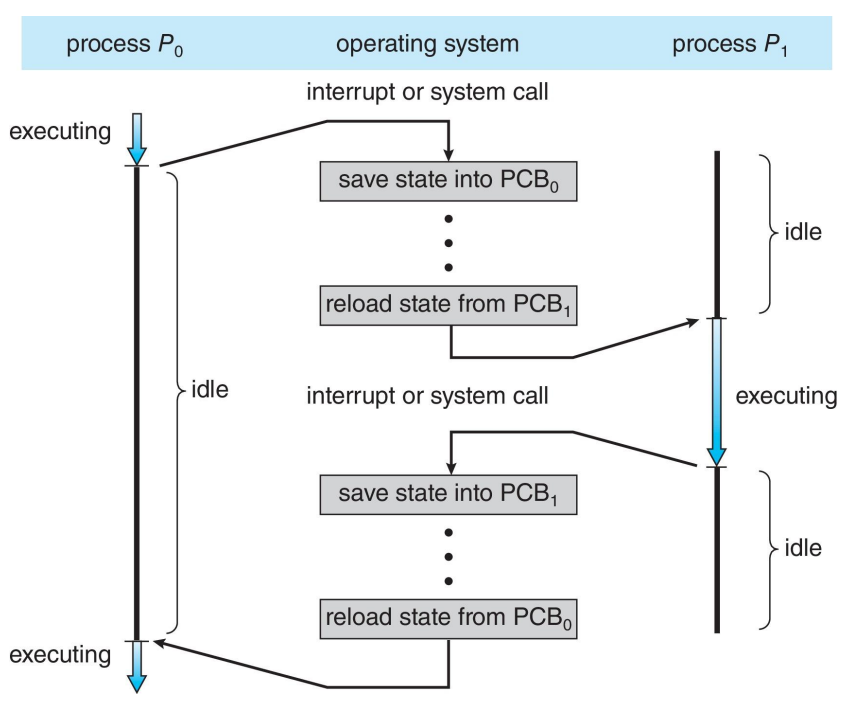
\includegraphics[width = .7\textwidth]{../res/imgs/processes/context_switch.png}
    \caption{Il context switch.}
    \label{fig:context_switch}
\end{figure}
È importante notare che il context switch tipicamente richiede anche un aggiuntivo utilizzo della memoria, che andremo a discutere nel capitolo \ref{main memory} quando discuteremo di \textit{paginazione} e \textit{swapping}.

% 
\subsection{Creazione di un processo}\label{creazione di un processo}
Al fine di creare un processo ce ne deve sempre essere uno iniziale (\textit{parent}) che genera il quello nuovo (\textit{child}). Ogni nuovo processo ha un identificativo, il \textbf{pid}, che distingue univocamente il processo creato. Al momento della creazione è possibile specificare alcune opzioni al fine di creare il processo child in un determinato modo. Prima tra tutte è l'opzione di \textbf{condivisione di risorse}, dove si può specificare se il figlio condivide le stesse risorse del genitore, un sottoinsieme oppure si può specificare che il figlio non condivida alcuna risorsa con il \textit{parent}. Inoltre si possono specificare le opzioni di \textbf{esecuzione}: si specifica se il figlio e il genitore possano essere eseguiti in maniera concorrente oppure se il \textit{parent} deve aspettare il termine dell'esecuzione del \textit{child}. Infine si può anche specificare lo \textbf{spazio degli indirizzi}, in particolare si sceglie se il figlio crea una copia identica della memoria utilizzata dal genitore oppure se carica un programma completamente nuovo.

Vediamo ora un esempio di creazione di un processo in \texttt{UNIX} (figura \ref{fig:fork}). Questo sistema operativo fornisce tre particolari \textit{system calls}:

\vspace{-5px}
\begin{itemize}
\setlength{\itemsep}{-.15 em}
    \item \texttt{fork()}: questa system call non fa altro che creare un processo. Il processo parent, dopo aver chiamato la funzione \texttt{fork()} viene duplicato. La funzione inoltre ritorna un valore intero, se questo valore è maggiore di zero vuol dire che ci troviamo all'interno del processo genitore; se invece il valore è zero vuol dire che il codice eseguito è all'interno del child. L'unico modo per distinguere se il processo è parent o child è attraverso il valore di ritorno di \texttt{fork}.
    \begin{figure}[h]
    \centering
    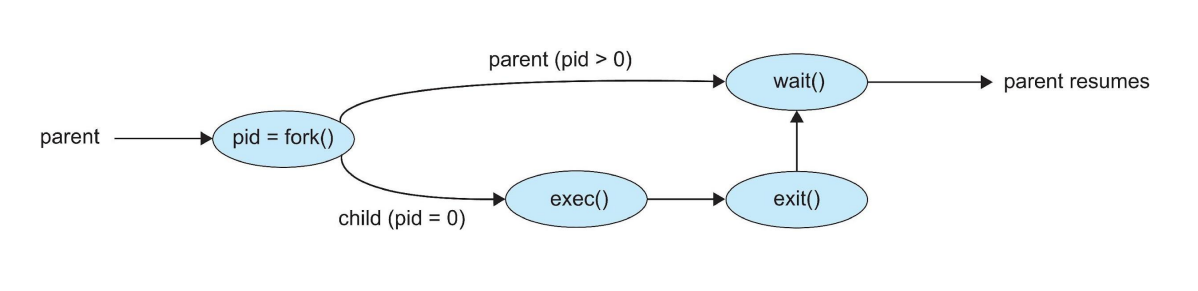
\includegraphics[width = .75\textwidth]{../res/imgs/processes/fork.png}
    \caption{Rappresentazione delle 3 \textit{system calls} fondamentali.}
    \label{fig:fork}
\end{figure}
    \item \texttt{exec()}: è una funzione utilizzata dal processo figlio nel caso in cui è necessario far partire un processo completamente diverso dal parent;
    \item \texttt{wait()}: è una systam call utilizzata dal genitore al fine di aspettare il termine dell'esecuzione del figlio.
\end{itemize}


%
\subsection{L'albero dei processi in Linux}
Come fa il sistema operativo a generare tutti i processi di cui ha bisogno? Ci deve sempre essere un processo iniziale, un programma all'inizio da cui tutti si genera. In particolare in Linux il primo processo da cui tutto è generato è chiamato \texttt{systemd} ed è il processo padre di tutti gli altri processi, quello il quale \texttt{pid} vale 1. Da \texttt{systemd}, \textit{forkando} processo dopo processo vengono generati tutti i processi necessari all'avvio del sistema, come il terminale, generando quindi un albero (figura \ref{fig:three_of_processes}).

\begin{figure}[h]
    \centering
    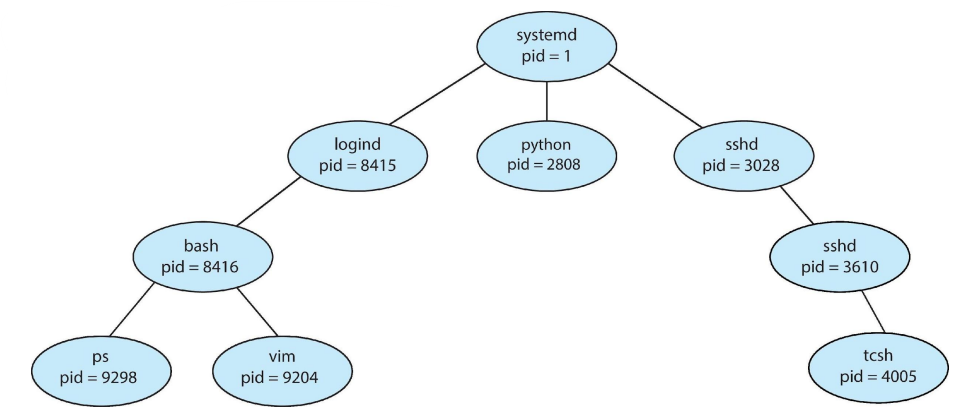
\includegraphics[width = .6\textwidth]{../res/imgs/processes/three_of_processes.png}
    \caption{L'albero dei processi generato da \texttt{systemd}.}
    \label{fig:three_of_processes}
\end{figure}

% 
\subsection{Terminazione di un processo}
Naturalmente, un processo può anche terminare. La terminazione del processo può essere spontanea (attraverso la \textit{system call} \texttt{exit}) e quindi il processo viene deallocato dal sistema operativo, oppure il processo può essere terminato dal genitore attraverso la system call \texttt{abort}. Questo di solito avviene quando il processo figlio supera il limite delle risorse allocate, quando la task che sta completando non è più richiesta oppure nel momento in cui il genitore termina e di conseguenza il sistema operativo termina anche i figli.

Come abbiamo visto in precedenza, esiste una funzione (\texttt{wait()}), che serve per evitare che il processo parent termini prima del processo child: la funzione infatti obbliga il parent ad aspettare che il child termini. Inoltre, se al termine di un processo child non c'è nessun processo parent che stava aspettando il termine del child, ci troviamo davanti ad un \textbf{processo zombie}. Infine, se il processo parent termina senza aspettare la terminazione del child, quest'ultimo è chiamato \textbf{orfano} e verrà terminato dal sistema operativo.

% 
\section{Comunicazione tra processi (IPC)}\label{IPC}
Passiamo ora a discutere i diversi modi per comunicare tra diversi processi. In alcuni casi avremo a che fare con processi indipendenti, altre volte invece necessiteremo di processi \textbf{cooperanti}. Per questi ultimi è necessario un modello di \textit{Inter-Process Communication}, chiamata anche \textbf{IPC}. In questo paragrafo ci occuperemo di due modelli: comunicazione tramite memoria condivisa e tramite il passaggio di messaggi.

% 
\subsection{Memoria condivisa}
Il primo modello di cui ci occuperemo è la tecnica di memoria condivisa. In questo modello, come possiamo notare anche dalla figura \ref{fig:shared_memory}, l'unica cosa di cui si fa carico il sistema operativo è l'assegnazione di una memoria che è condivisa tra i processi A e B.
\begin{figure}[h]
    \centering
    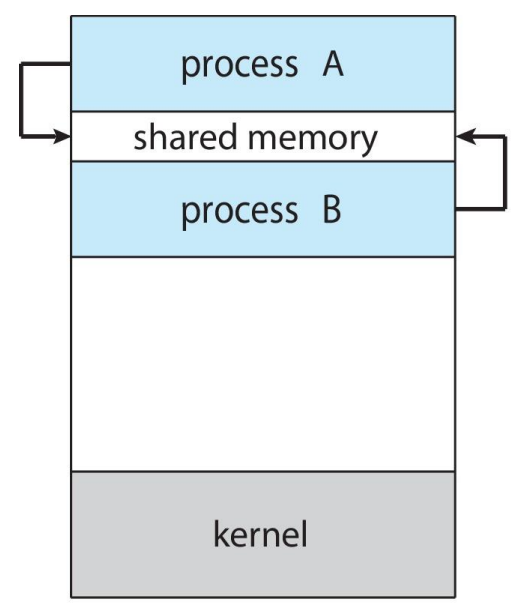
\includegraphics[width = .25\textwidth]{../res/imgs/processes/shared_memory.png}
    \caption{Il modello di memoria condivisa per IPC.}
    \label{fig:shared_memory}
\end{figure}
Ciò significa che la comunicazione è molto veloce tra i due processi in quanto non c'è nessun intermediario tra i due. Allo stesso tempo però è più facile che si generino errori come la sovrascrittura di valori e in genere problemi di sincronizzazione con i dati (come la \textit{race condition}, vedi capitolo \ref{sincronizzazione}) in quanto il sistema operativo non ha alcun tipo di controlla sulla memoria secondaria.

Partiamo ora da un esempio di questo modello al fine di ottenere informazioni più dettagliate: stiamo infatti parlando del problema \texttt{Producer - Consumer}. Ipotizziamo quindi che due processi abbiano dello spazio in memoria condiviso; la comunicazione attraverso questa memoria può avvenire in due modi:
\vspace{-5px}
\begin{itemize}
\setlength{\itemsep}{-.15 em}
    \item \textbf{unbounded}, ovvero che il produttore continua a generare dati da mettere nell'area condivisa, e che il consumatore continua ad utilizzare quei dati fino a che non finiscono (al più attende la creazione di altri dati).
    \item \textbf{bounded}, dove si ha un \textbf{buffer} che entrambi devono aspettare: il consumer attende che ci siano dati nel buffer e il producer aspetta nel momento in cui il buffer è pieno. 
\end{itemize}

% 
\subsection{Passaggio di messaggi}
In questo secondo caso invece il sistema operativo si prende carico di gestire la coda dei messaggi (\textbf{message queue}) che vengono scambiati tra i due processi (figura \ref{fig:message_passing}). In questo caso è il kernel che fa da intermediario tra i due e di conseguenza la velocità di comunicazione sarà ridotta dall'\textbf{overhead}.
\begin{figure}[h]
    \centering
    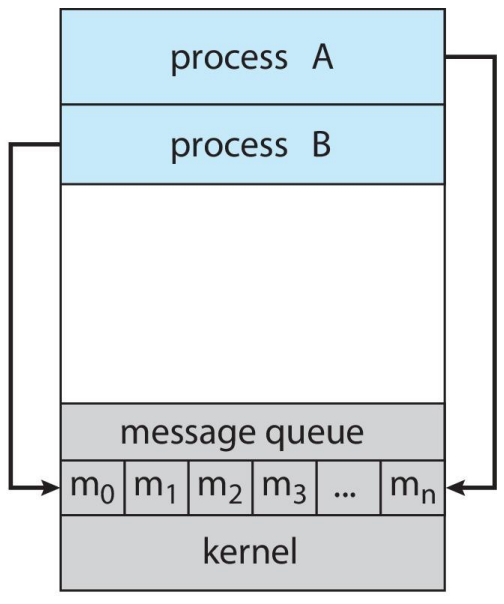
\includegraphics[width = .25\textwidth]{../res/imgs/processes/message_passing.png}
    \caption{Il modello di memoria condivisa per IPC.}
    \label{fig:message_passing}
\end{figure}
Allo stesso tempo però il kernel garantisce la sincronizzazione e la correttezza tra i messaggi scambiati e di conseguenza è un modello più sicuro. 

Discutiamo ora più dettagliatamente questo modello. In particolare, sono fornite due operazioni fondamentali: \texttt{send(message)} e \texttt{recive(message)}. Ciò nonostante la comunicazione di tali messaggi fa sorgere diversi dubbi e domande legate alla progettazione: come sono stabilite le connessioni? qual è la sua capacità? è unidirezionale o bidirezionale? la dimensione del messaggio è fissa o variabile? un collegamento è associato solo a 2 processi o a più? Per rispondere a queste domande andiamo a vedere l'implementazione di questo modello che può essere di due tipi.

Quando si parla di comunicazione \textbf{diretta}, si intende che i processi specifichino esplicitamente il destinatario del messagio: \texttt{send(Q, message)} e \texttt{recive(P, message)}. Nella comunicazione \textbf{indiretta} invece si ha a che fare con un \textbf{buffer}, chiamato anche porta, il quale ha un ID unico tra gli altri. In questa implementazione due processi si possono parlare solo se condividono questo buffer (\textbf{mailbox}). Se più processi condividono la stessa mailbox si ha quindi un link che collega diversi processi, inoltre attraverso questa porta il collegamento è bidirezionale in quanto un processo può sia spedire un messaggio che riceverlo. Con la comunicazione indiretta le primitive però sono diverse: una volta creata la porta (chiamiamola \texttt{A}, per comodità), al fine di scambiare i messaggi è necessario utilizzare le operazioni \texttt{send(A, message)} e \texttt{recive(A, message)}.


\chapter{Threads}
Partiamo con il distinguere un thread da un processo. Il thread è un \textbf{filo di esecuzione}: in un processo ci possono essere diversi thread i quali possono avere dei diversi \textit{pattern} per ciascuna esecuzione.

\subsubsection*{Perché?}
I thread sono entità più semplici rispetto ai processi e sono quindi più facili da gestire. Grazie ai thread si ottengono diversi vantaggi:
\vspace{-5px}
\begin{itemize}
\setlength{\itemsep}{-.25 em}
    \item Il sistema è più \textbf{recettivo};
    \item Dato che le risorse sono condivise è più facile gestirle;
    \item Richiede meno risorse rispetto alla creazione di un processo;
    \item Può utilizzare tutti i \textit{core} messi a disposizione dal sistema (\textit{multicore programming}).
\end{itemize}

\noindent Per esempio, al posto di far eseguire 4 processi differenti è molto meglio eseguire un processo con 4 thread differenti: in questo modo si evita di allocare in memoria 4 volte le stesse risorse che, grazie all'utilizzo dei thread, sono allocate solo una volta. 
% 
\section{Concorrenza e parallelismo} \label{parallelismo}
Quando parliamo di \textbf{multicore programming} è necessario fare una netta distinzione tra il significato di concorrenza e parallelismo. Con \textbf{parallelismo} si intende che un sistema è in grado di preformare più di un compito in maniera simultanea (tipico dei sistemi multicore). Con \textbf{concorrenza} si intende la possibilità di far progredire più di un compito (non in maniera simultanea).

Come possiamo vedere della figura \ref{fig:concorrenza}, quando parliamo di concorrenza ci riferiamo ad un singolo core che esegue a frammenti più thread diversi.
\begin{figure}[!h]
    \centering
    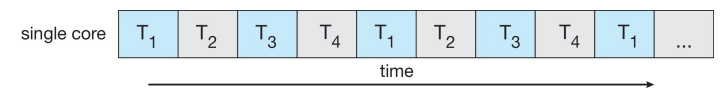
\includegraphics[width=.7\textwidth]{../res/imgs/threads/concorrenza.png}
    \caption{Esempio di concorrenza tra 4 processi.}
    \label{fig:concorrenza}
\end{figure}

Quando invece facciamo riferimento al parallelismo (figura \ref{fig:parallelismo}) indichiamo la capacità del sistema di effettivamente riuscire ad eseguire parallelamente diversi thread. 
\begin{figure}[!h]
    \centering
    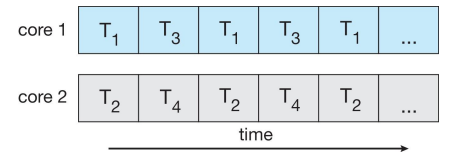
\includegraphics[width=.5\textwidth]{../res/imgs/threads/parallelismo.png}
    \caption{Esempio di parallelismo in un sistema dual core.}
    \label{fig:parallelismo}
\end{figure}
Si osserva che le due pratiche non sono esclusive: notiamo che il core 1 esegue in maniera concorrente T1 e T3, mentre il core 2 esegue in maniera concorrente T2 e T4.

\subsection{Tipi di parallelismo}
Possiamo dividere i parallelismi in due tipi. Il primo, chiamato \textbf{data parallelism} (figura \ref{fig:data_parallelism}) implica un sottoinsieme preciso di dati sia distribuito per ogni core. In altre parole, avendo a che fare un un largo database, lo si suddivide in parti e ciascuna viene assegnata ad un core. Tale core potrà operare solo in quella porzione di dati
\begin{figure}[!h]
    \centering
    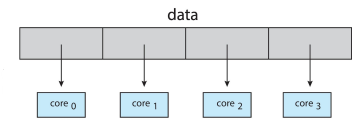
\includegraphics[width = .5\textwidth]{../res/imgs/threads/data_parallelism.png}
    \caption{Esempio di parallelismo di dati.}
    \label{fig:data_parallelism}
\end{figure}

\noindent Il secondo tipo di parallelismo è detto \textbf{task parallelism}, rappresentato in figura \ref{fig:task_parallelism}. Questo tipo di parallelismo concede la memoria condivisa a ciascun core solo che ogni core ha un compito ben preciso: un core sarà ottimizzato per la scrittura, un altro sarà più veloce in lettura e così via.
\begin{figure}[!h]
    \centering
    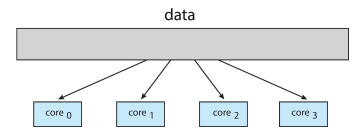
\includegraphics[width=.5\textwidth]{../res/imgs/threads/task_parallelism.png}
    \caption{Esempio di parallelismo di compiti.}
    \label{fig:task_parallelism}
\end{figure}
% 
\subsection{Legge di \textit{Amdahl}}
La legge di \textit{Amdahl} è una funzione che mette in relazione due variabili importanti:
\vspace{-5px}
\begin{enumerate}
\setlength{\itemsep}{-.15 em}
    \item \textbf{S}, ovvero la percentuale di codice che non può essere parallelizzato, ovvero codice \textbf{seriale} (di conseguenza il numero di codice che può essere parallelizzato è $1 - S$);
    \item \textbf{N}, che rappresenta il numero di core disponibili. 
\end{enumerate}

\noindent Con questi due dati abbiamo la possibili di calcolare lo \textit{\textbf{speedup}} attraverso la seguente formula:
\begin{equation*}
    \text{\textit{speedup}} \leq \frac{1}{S + \frac{1 - S}{N}}
\end{equation*}

\noindent Osservando la formula osserviamo che se se la percentuale di codice seriale tende a zero e il numero di core tende a infinito, lo \textit{speedup} sarebbe infinito. Questa però è una situazione utopica: non esistono casi in cui si è privi di codice seriale.

Osserviamo quindi il seguente grafico (figura \ref{fig:speedup}) che mostra lo \textit{speedup} all'aumentare del numero di core, essendo a conoscenza della percentuale di codice seriale.
\begin{figure}[!h]
    \centering
    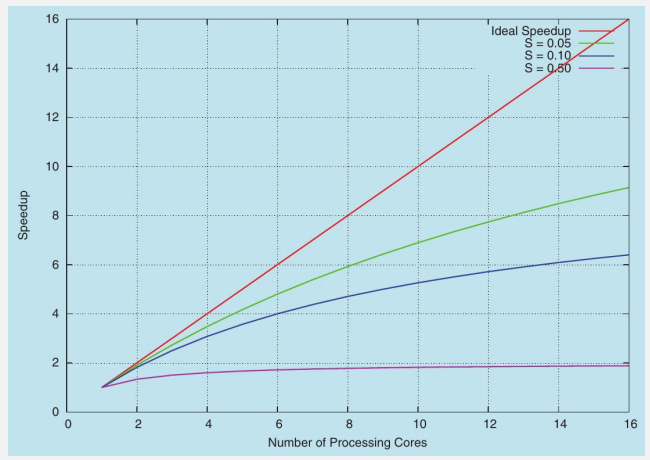
\includegraphics[width=.6\textwidth]{../res/imgs/threads/speedup.png}
    \caption{Il grafico che descrive lo \textit{speedup} a seconda della percentuale di codice seriale.}
    \label{fig:speedup}
\end{figure}
Notiamo che quando la percentuale di codice seriale è circa la metà non ha importanza il numero di core del sistema: lo speedup rimarrà pressoché invariato. Anche solo con il 5\% di codice seriale notiamo un forte abbassamento rispetto allo speedup ideale. È evidente quindi che l'aumento di core non causa l'aumento di speedup, sopratutto in una situazione dove il codice seriale è molto. 
% 
\section{Modelli multithreading}
È importante fare una distinzione tra due classi principali di thread: \textbf{user threads} e \textbf{kernel threads}. La principale differenza tra i due è che i kernell threads hanno molti più privilegi rispetto a quelli utente. Esistono quindi dei modelli che cercano di associare agli user threads i kernell threads al fine di sfruttare al meglio il principio di \textit{multithreading}.

\subsection{Many-to-One}
In questa prima architettura, il kernell mette a disposizione solo un thread che è collegato e deve soddisfare tutte le richieste di tutti gli user threads (figura \ref{fig:many_to_one}).
\begin{figure}[!h]
    \centering
    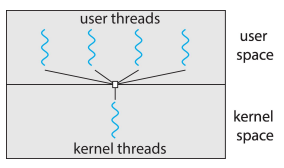
\includegraphics[width = .5\textwidth]{../res/imgs/threads/many_to_one.png}
    \caption{Il modello di \textit{multithreading} molti a uno.}
    \label{fig:many_to_one}
\end{figure}
È evidente che l'efficienza di questo modello non è il suo forte: sono presenti diversi thread utente ai quali deve rispondere solamente un thread del kernel. Basta pesare al fatto che se il kernel thread è in attesa di un input esterno, tutti gli user thread sono bloccati (\textbf{collo di bottiglia}). Questo modello è infatti poco utilizzato dato che non sfrutta le potenzialità del \textit{multicore}. 
% 
\subsection{One-to-One}
In questa architettura (figura \ref{fig:one_to_one}), quando viene creato uno user thread, il suo rispettivo kernel thread viene creato; così facendo esiste un kernell thread associato ad ogni user thread. 
\begin{figure}[!h]
    \centering
    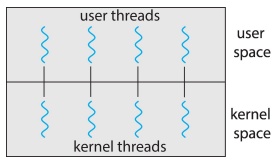
\includegraphics[width = .5\textwidth]{../res/imgs/threads/one_to_one.png}
    \caption{Il modello di \textit{multithreading} uno a uno.}
    \label{fig:one_to_one}
\end{figure}
Ad ogni modo ci possono essere alcune restrizioni in modo da evitare la creazioni di troppi kernel threads (e quindi limitare la creazione di user threads). È comunque evidente che questo modello è sicuramente più \textbf{efficace} del modello precedente in quanto fornisce la possibilità di sfruttare a piano un sistema multicore.
% 
\subsection{Many-to-Many}
L'ultimo modello è un buon compromesso tra il modello \textit{Many-to-One} e il modello \textit{One-to-One}. Il modello molti a molti (figura \ref{fig:many_to_many}) fornisce diversi vantaggi ed è più flessibile rispetto ai primi due. Non esiste infatti la corrispondenza univoca, generalmente si hanno più user threads che fanno riferimento ad alcuni kernell threads (è come se una sala da 20 clienti fosse gestita da 5 camerieri). 
\begin{figure}[!h]
    \centering
    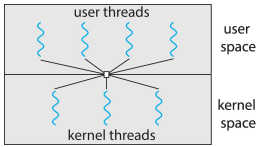
\includegraphics[width = .5\textwidth]{../res/imgs/threads/many_to_many.png}
    \caption{Il modello di \textit{multithreading} molti a molti.}
    \label{fig:many_to_many}
\end{figure}
È possibile infatti controllare in maniera più efficace i kernell thread e questo rende il modello \textit{Many-to-Many} molto \textbf{robusto}. Ad ogni modo la sua implementazione è molto più complessa rispetto ai modelli precedenti.

Per questo, a volte, si fa riferimento ad un \textit{ibrido} tra il modello \textit{Many-to-Many} e il modello \textit{One-to-One}: stiamo parlando del \textbf{Two-level model} che consente sia la corrispondenza \textit{1 a 1} che la corrispondenza \textit{N a M}.

% 
\section{Librerie di thread}
In questa piccola sezione ci interessiamo alle libreire disponibili per la creazione e la gestione di threads. Queste possono essere di due tipi:
\begin{itemize}
\setlength{\itemsep}{-.15 em}
    \item Librerie in \textbf{user space}, dove i thread sono gestiti completamente a livello utente (come nel caso di \texttt{Pthreads});
    \item Librerie di tipo \textbf{kernel-level} che sono supportate dal sistema operativo e si appoggiano al kernel attraverso le \textit{system calls}; questo comporta un livello maggiore di complessità nel kernell ma il programmatore ha meno da implementare.
\end{itemize}

\noindent Spendiamo due parole su \texttt{POSIX Threads}. Questa, non è propriamente una libreria ma è un insieme di specifiche (non implementazioni!) che aiuta con la creazione e la gestione di thread. \texttt{POSIX Threads} fornisce specifiche sia a livello di utente che a livello di kernel.

% 
\section{Threading implicito}
Cerchiamo ora di cambiare approccio: attraverso le librerie l'approccio era esplicito, stava al programmatore l'implementazione e/o la gestione dei thread. Nel momento in cui si fa riferimento a più threads, diventa sempre più difficile controllare la correttezza del codice. Ecco che si è pensato ad un altro approccio: il threading \textbf{implicito}. Con questo approccio i thread sono gestiti maggiormente dal compilatore oppure da librerie \textit{run-time} le quali si occupano di creare e gestire i thread. In questa sezione vedremo alcuni dei metodi utilizzati per ottenere il threading implicito. 
% 
\subsection{Modello fork-join}
Questo tipo di modello si ispira alla creazione di processi (paragrafo \ref{creazione di un processo}). In questo modello, diversi threads sono divisi e, una volta che sono terminati, vengono uniti (figura \ref{fig:fork_join}). La divisione dei threads è una scelta presa completamente dalla libreria.
\begin{figure}
    \centering
    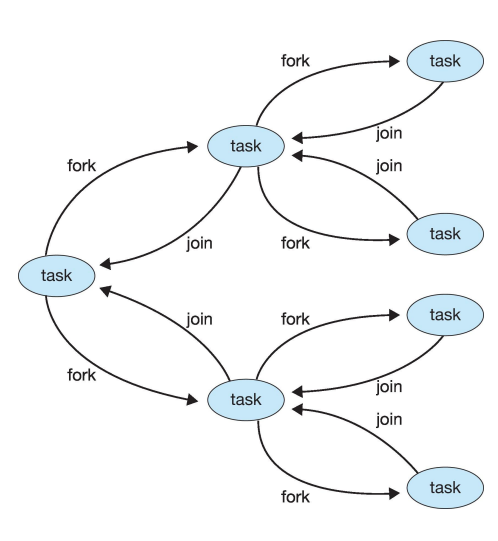
\includegraphics[width = .4\textwidth]{../res/imgs/threads/fork_join.png}
    \caption{Rappresentazione grafica del modello fork-join per la risoluzione di un task.}
    \label{fig:fork_join}
\end{figure}
Come possiamo notare dalla figura \ref{fig:fork_join}, in questo caso, la libreria sceglie un task da far risolvere ad un thread dove, eventualmente verrà splittata in altri due thread (che vengono appositamente creati) e così via fino a che il task non sia completamente risolto.
% 
\subsection{Thread pools e OpenMP}
Altri due modelli molto importanti sono \textit{thread pools} e \texttt{OpenMP}. Nel primo caso la libreria mette a disposizione un numero di thread (\textit{pool} di thread) che attendono un  task da risolvere. In questo modo, dato che i thread sono già pronti, non si spreca tempo per l'effettivo processo di creazione. Inoltre il problema della limitazione dei thread è risolto in quanto una volta creati quelli per la \textit{pool}, non vengono creati altri thread. 

Quando parliamo di \texttt{OpenMP} invece parliamo di una serie di \textbf{direttive} per il compilatore e un insieme di librerie per \texttt{C}, \texttt{C++} e \texttt{FORTRAN}. Questo modello fornisce tutte le risorse per la condivisione della memoria tra i thread e i parallelismi. Essendo delle direttive, queste devo essere proprio scritte nel codice; per esempio: \texttt{\#pragm omp parallel}.
% 
\section{Problematiche}
Come vedremo in questo paragrafo, anche i thread portano a delle problematiche che devono essere gestite come, per esempio, l'interruzione di tali e il modo di implementare l'eliminazione di un thread.

\subsection{Semantica \texttt{exec} e \texttt{fork}}
Il primo dubbio che è necessario chiarire è il comportamento durante la chiamata della funzione \texttt{exec()}: se si fa una chiamata alla funzione \texttt{exec()}, vengono rimpiazzati tutti i thread del processo oppure solo il thread su cui è stata chiamata \texttt{exec}? Generalmente la funzione \texttt{exec} cancella il processo in esecuzione e, di conseguenza, tutti i sui thread.

Il secondo dubbio, riguarda la funzione \texttt{fork()}: se si fa una chiamata a \texttt{fork()} ad un processo multithread, si effettua una copia a tutti i thread del processo oppure solo al thread su cui è stata chiama la funzione? La risposta a questa domanda è che dipende dall'obiettivo della funzione \texttt{fork()}:
\vspace{-5px}
\begin{itemize}
\setlength{\itemsep}{-.15 em}
    \item Se la funzione deve cambiare subito il codice attraverso \texttt{exec()}, non vale la piena copiare tutti i thread se tanto si si che verranno eliminati.
    \item Se invece il nuovo processo deve supportare anch'esso il multithreading, allora ha senso effettuare una coppia di tutti i thread e non solo del thread su cui è stata chiamata la funzione
\end{itemize}
% 
\subsection{Segnalazione ed eliminazione}
I segnali sono usati per notificare un processo che un determinato evento è accaduto. Tali segnali però debbono essere gestiti: ecco che emerge la figura del \textbf{signal handler} che può essere di \textbf{default} oppure \textbf{user-defined}, ovvero definito dall'utente. Generalmente ogni segnale ha il suo specifico \textit{default handler} che è utilizzato anche dal kernel. Cosa succede però nel caso in cui il sistema è multi-threading? Ci sono diverse opzioni:
\vspace{-5px}
\begin{enumerate}
\setlength{\itemsep}{-.15 em}
    \item Spedire il segnale al thread ad esso compatibile;
    \item Propagare il segnale ad ogni thread del processo;
    \item Mandare il segnale ad dei thread specifici del processo;
    \item Assegnare ad uno specifico thread il compito di ricevere i segnali degli altri thread.
\end{enumerate}

\noindentÈ inoltre importante riuscire a gestire la \textbf{cancellazione} dei thread. Questi però devono attivare la possibilità di essere cancellati: in altre parole, se un thread ha la cancellazione disabilitata non potrà essere cancellato fino a che non viene riattivata. Nel momento in cui la cancellazione è attivata, il thread può essere cancellato attraverso due tecniche:
\vspace{-5px}
\begin{itemize}
\setlength{\itemsep}{-.15 em}
    \item \textbf{Asincrona}, ovvero il thread termina immediatamente;
    \item \textbf{Deferred} che significa \textit{posticipata}. Può ritornare utile nel momento in cui il thread sta compiendo un'operazione delicata (chiusura di un file) e non ha la possibilità di terminare immediatamente. 
\end{itemize}




\pagebreak
\chapter{CPU Scheduling} \label{CPU scheduling}
In questa sezione ci occupiamo di tutti gli aspetti che concernono lo scheduling del processore, ovvero la pratica secondo la quale, attraverso dei precisi criteri, si sceglie quale processo all'interno della \textit{ready queue} verrà eseguito.

\section{Nozioni fondamentali}
Prima di iniziare a discutere di scheduling vero e proprio è necessario avere chiari alcuni concetti importanti.

\paragraph{Burst.}
La prima è la nozione di burst. Chiamiamo \textbf{CPU burst} il periodo di tempo nel quale un processo esegue operazioni all'interno della CPU; diversamente, l'\textbf{I/O burst} è il tempo che il processo spende interfacciandosi con le periferiche di input e output. In particolare, un processo che occupa per molto tempo la CPU si dice \textit{CPU bounded}, mentre nel caso di I/O si parla di un processo \textit{I/O bounded}. In questo capito ci occupiamo solo di CPU burst.
% 
\paragraph{CPU scheduler.}
Il CPU scheduler è il responsabile dell'organizzazione e dell'ordinamento della \textbf{coda dei processi} (figura \ref{fig:process'life}). Le decisioni su quale processo deve essere eseguito prima stanno a lui. Questo tipo di decisioni avvengono generalmente quando un processo:
\vspace{-5px}
\begin{enumerate}
\setlength{\itemsep}{-.15 em}
    \item Passa dallo stato \textit{running} a \textit{waiting};
    \item Passa da \textit{running} allo stato \textit{ready};
    \item Passa dallo stato \textit{waiting} allo stato \textit{ready};
    \item Termina.
\vspace{-5px}
\end{enumerate}
Osserviamo che per i punti 1 e 4 non è presente una vera e propria decisione: un nuovo processo deve essere messo in esecuzione. Questo non vale per i punti 2 e 3 dove si fa una decisione.
\begin{figure}[h]
    \centering
    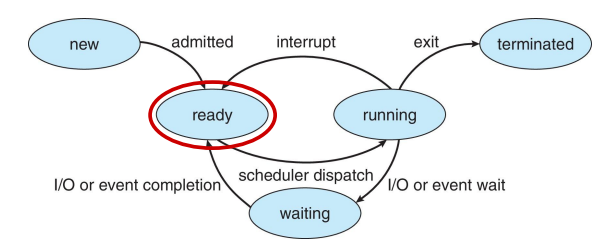
\includegraphics[width = .65\textwidth]{../res/imgs/CPU scheduling/dispatcher.png}
    \caption{Lo scheduler entra in gioco nel passaggio da ready a running.}
    \label{fig:process'life}
\end{figure}
% 
\paragraph{Preemption.}
Ci sono due macro gruppi di scheduling: preemptive e non. Uno scheduling è detto \textbf{non preemptive} nel momento in cui un processo non può essere fermato. In altre parole, quando la CPU è assegnata ad un processo, questo la utilizza fino a che non è terminato. Differentemente, uno scheduling è detto \textbf{preemptive} quando un processo può essere fermato per dare precedenza ad un altro per poi essere fatto ripartire: questo tipo di scheduling è sicuramente più performante e moderno; è infatti utilizzato nei sistemi operativi più diffusi come Windows, MacOS, Linux e altri. Ciò porta comunque a delle situazioni indesiderate come le \textbf{race conditions}: poniamo il caso di avere due processi che condividono dei dati; immaginiamo che il primo processo stia aggiornando questi dati ma allo stesso tempo il secondo processo li stia utilizzando. Questo è un problema dato che il processo due sta utilizzando dei dati che non sono consistenti dato che sono in fase di aggiornamento dal processo uno. Come vedremo nel capitolo \ref{sincronizzazione}, questo è un problema di sincronizzazione che va risolto.
% 
\paragraph{Dispatcher.}
Nel momento in cui lo scheduler ha scelto quale processo verrà eseguito, il dispatcher si occupa di cambiare il processo nella CPU. In particolare viene effettuato il \textit{context switch} (\ref{context_switch}), passa in \textit{user mode} e va alla giusta locazione del programma per iniziare la sua esecuzione. Durante tutto ciò la CPU però non lavora: è importante quindi minimizzare questa latenza e fare in modo che non se ne effettuino un numero troppo elevato al fine di mantenere un alta percentuale di utilizzo della CPU.
% 
\section{Algoritmi non preemptive}
In questo paragrafo ci occupiamo dei primi algoritmi non preemptive, ovvero gli algoritmi che non fermano i processi che sono in esecuzione. 

\subsection{First-Come First-Served (FCFS)}
Questo è l'algoritmo più banale da implementare: il primo processo che entra nella coda sarà anche il primo ad essere eseguito. Questo algoritmo ha un approccio praticamente identico al \textbf{FIFO} (\textit{First In First Out}). Attraverso un semplice esempio, possiamo osservare che questo algoritmo non è efficiente. Poniamo che entrino nella coda 3 processi: $P_1$, di durata 24 unità di tempo (in genere millisecondi) e $P_2$ e $P_3$ con durata di esecuzione 3.  
\begin{figure}[h]
    \centering
    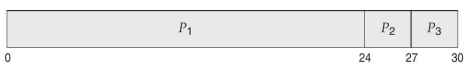
\includegraphics[width = .7\textwidth]{../res/imgs/CPU scheduling/FCFS.png}
    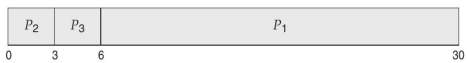
\includegraphics[width = .7\textwidth]{../res/imgs/CPU scheduling/FCFS2.png}
    \caption{Diagramma di \textit{Gantt} dell'algoritmo FCFS.}
    \label{fig:FCFS}
\end{figure}
Osservando la figura \ref{fig:FCFS} è banale notare che se $P_1$ fosse arrivato in coda per ultimo, i processi $P_2$ e $P_3$ avrebbero aspettato meno.
Possiamo dimostrarlo anche in maniera più matematica, attraverso dei brevi calcoli. Nel primo caso $P_1$ ha aspettato 0 prima di essere eseguito, $P_2$ ha aspettato l'esecuzione di $P_1 = 24$ mentre $P_3$ ha aspettato l'esecuzione di $P_1 + P_2 = 24 + 3 = 27$. Se provassimo a fare una media del tempo di attesa otteniamo:
\begin{gather*}
    \langle T\rangle = \frac{0 + 24 + 27}{3} = 17
\end{gather*}
Nel secondo caso invece la situazione migliora notevolmente in quanto $P_2$ aspetta 0, $P_3$ aspetta solamente l'esecuzione di $P_2 = 3$ e infine $P_1$ attende l'esecuzione di $P_2 + P_3 = 3 + 3 = 6$. Attraverso la stessa espressione matematica otteniamo che l'attesa media in questo caso diventa:
\begin{gather*}
    \langle T \rangle = \frac{6 + 0 + 3}{3} = 3
\end{gather*}

Diversi sono i problemi di questo algoritmo. Prima di tutto può generare il \textbf{convoy effect} (effetto convoglio): se viene eseguito un processo \textit{I/O bounded}, tutti gli altri processi in coda devono aspettare che questo si "sblocchi" generando quindi un rallentamento generale. In secondo luogo, questo algoritmo di scheduling dipende dall'ordine di entrata dei processi e di conseguenza \textbf{non} è nemmeno possibili analizzare in modo \textbf{deterministico} le prestazioni dell'algoritmo.
% 
\subsection{Shortest-Job-First (SJF)}\label{SJF}
Come abbiamo notato dalla figura \ref{fig:FCFS}, se i processi più bervi sono eseguiti prima, il tempo medio di attesa $\langle T \rangle$ si abbassa. Implementiamo quindi un algoritmo che dia la precedenza ai processi con il tempo di esecuzione più breve tra quelli che sono presenti in coda. In questo algoritmo stiamo assumendo che siamo a conoscenza del CPU burst time di ciascun processo: si osserva che stiamo facendo un'ipotesi, spesso questo dato non è a disposizione. Se tutti i CPU burst sono conosciuti, l'algoritmo fornisce il minor tempo medio di attesa di un insieme finito di processi.

Il funzionamento di questo algoritmo è molto semplice: in base ai processi arrivati in coda, questi, prima di essere eseguiti, vengono riordinati in base al loro tempo di burst. Per esempio, poniamo di avere in coda un processo $P_1$ con un burst time di 6, $P_2$ da 8, $P_3$ da 7 e $P_4$ da 3.
\begin{figure}[h]
    \centering
    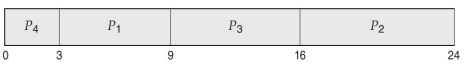
\includegraphics[width = .7\textwidth]{../res/imgs/CPU scheduling/SJF.png}
    \caption{Diagramma di \textit{Gantt} dell'algoritmo SJF.}
    \label{fig:SJF}
\end{figure}
Osservando la figura \ref{fig:SJF} notiamo che i processi sono stati riordinati in modo tale da minimizzare il tempo medio d'attesa. In questo esempio il processo $P_4$ attende 0, il processo $P_1$ attende l'esecuzione di $P_4 = 3$, il processo $P_3$ aspetta la conclusione di $P_4 + P_1 = 3 + 6 = 9$ e infine il processo $P_2$ aspetta $P_4 + P_1 + P_3 = 3 + 6 + 7 = 16$. Ecco che il tempo di attesa medio diventa:
\begin{gather*}
    \langle T \rangle = \frac{3 + 16 + 9 + 0}{4} = 7
\end{gather*}

Anche in questo caso però se durante l'esecuzione è in coda un processo con un burst molto alto e entrano solo processi con un burst basso, è probabile che si verifichi una situazione di attesa perenne (chiamata \textbf{starvation}); vedremo, nel corso di questo capitolo, come ciò può essere evitato (\ref{priority scheduling}).
% 
\subsection{Stima del \textit{CPU burst time}}
Come abbiamo affermato poco fa, quasi mai il burst time è a disposizione. Si è quindi trovato un modo per stimare al meglio il burst time di un processo, in base ai processi che sono stati eseguiti in precedenza. Il metodo utilizzato è chiamato \textbf{exponential averaging} il quale, in essenza, dà peso maggiore ai processi eseguiti da poco tempo e, pian piano, più i processi sono remoti, meno influenza hanno sulla stima. Le variabili in gioco nella formula sono:
\vspace{-5px}
\begin{itemize}
\setlength{\itemsep}{-.15 em}
    \item $t_i$ indica la durata del CPU burst del processo \textit{i}-esimo, dove $i\in[0,n]$, dove $n$ indica il numero di processi;
    \item $\tau_{n+1}$ rappresenta la stima, la predizione (\textit{guess}), che si calcola sul processo che si sta per eseguire;
    \item $\alpha$ che è un coefficiente che indica quanto pesa la storia dei processi. Quando questo coefficiente è basso, la storia recente non conta, mentre quando è alto, la storia recente ha più peso (con $\alpha = 1$ si ha che solo l'ultimo processo influisce sulla stima). Generalmente si utilizza il valore $\alpha = \frac{1}{2}$.
\end{itemize}
Nel caso generale, con $n$ processi si ha che per stimare il burts dell' $n+1$-esimo:
\begin{gather*}
    \tau_{n + 1} = \alpha t_n + (1 - \alpha)\alpha t_{n - 1} + ... \\
                    + (1 - \alpha)^i\alpha t_{n - i} + ...\\
                    + (1 - \alpha)^{n + 1}\tau_0
\end{gather*}

Osserviamo ora la figura \ref{fig:CPU burst estimation} che rappresenta come viene effettuata la \textit{guess} in base alla storia dei processi ($\alpha = .5$).
\begin{figure}[h]
    \centering
    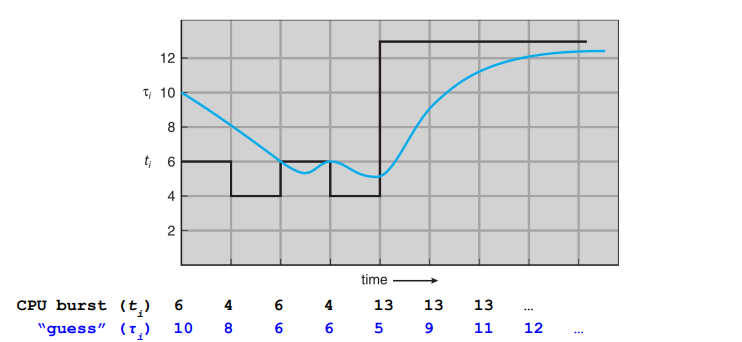
\includegraphics[width = .75\textwidth]{../res/imgs/CPU scheduling/CPU_burst_estimation.png}
    \caption{Grafico che indica come viene stimato il burst di un processo.}
    \label{fig:CPU burst estimation}
\end{figure}
La prima colonna composta dalla coppia $\binom{6}{10}$ è la colonna "base", la partenza del nostro grafico. Con questi due dati, si calcola la seconda colonna $\binom{4}{8}$, dove $ 8 = \frac{10 + 6}{2}$; a questo punto si può calcolare la terza colonna $\binom{6}{6}$, dove il secondo $6 = \frac{4 + 8}{2}$. Così facendo si è in grado di calcolare una buona stima per il CPU burst time del processo corrente.

% 
\section{Algoritmi preemptive}
In questo secondo paragrafo discutiamo invece di due algoritmi preemptive, ovvero algoritmi che possono fermare l'esecuzione di un processo per favorirne un altro.

% 
\subsection{Shortest-Remaining-Time-First (SRTF)}
Il primo algoritmo che andremo a discutere è la versione preemptive del SJF: in questo caso viene servito per primo il processo al quale manca minor tempo per essere completato. Quindi se si sta eseguendo un processo $P$ e arriva un processo $Q$ il quale burst time è minore rispetto al burst time che manca a $P$ per terminare, quest'ultimo viene fermato per dare la precedenza a $Q$. Una volta terminata l'esecuzione di $Q$, il processo $P$ riprede da dove era stato fermato in precedenza. Prendiamo in considerazione i seguenti 4 processi:
\begin{table}[h]
    \centering
    \begin{tabular}{c c c}
        \textbf{Processo} & \textbf{Tempo di arrivo} & \textbf{Stima burst time} \\\hline
        $P_1$ & 0 & 8 \\
        $P_2$ & 1 & 4 \\
        $P_3$ & 2 & 9 \\
        $P_4$ & 3 & 5 \\\hline
    \end{tabular}
\end{table}

Osservando la figura \ref{fig:SRTF}, cerchiamo di capire come si comporta questo algoritmo nel momento in cui i 4 processi sono inseriti all'interno della coda.
\begin{figure}[h]
    \centering
    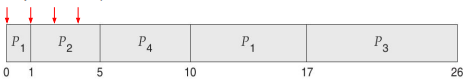
\includegraphics[width = .75\textwidth]{../res/imgs/CPU scheduling/SRTF.png}
    \caption{Diagramma di \textit{Gantt} dell'algoritmo SRTF.}
    \label{fig:SRTF}
\end{figure}
Al tempo zero arriva in coda il processo $P_1$, di durata 8. Al tempo 1 arriva in coda il processo $P_2$ che ha una durata di 4. A $P_1$ rimangono ancora $8 - 1 = 7$ unità di tempo prima di terminare, mentre a $P_2$ ne servono solo 4. $P_1$ viene quindi fermato e $P_2$ inizia la sua esecuzione (si effettua un \textit{depatching}). Al tempo 2 e al tempo 3 sono aggiunti alla coda $P_3$ e $P_4$ i quali però hanno un burst time maggiore rispetto a $P_2$ che quindi termina l'esecuzione al tempo $1 + 4 = 5$. A questo punto rimangono $P_1$, $P_3$ e $P_4$. Viene eseguito $P_4$ in quanto il suo burst (5) è minore rispetto a quello di $P_1$ (7) e $P_3$ (9). Terminata l'esecuzione di $P_4$ inizia quella di $P_1$ e poi quella di $P_3$.

Osserviamo che con questo algoritmo può capitare che sia in esecuzione un processo con un tempo di burst molto elevato e che poi continuino ad arrivare dei processi con un tempo di burst ridotto. In questo caso, il processo con il tempo maggiore verrebbe sempre interrotto dagli altri processi e non riuscirebbe mai a terminare andando quindi in una situazione di \textbf{starvation}. Come vedremo, una soluzione è questo problema è fornita dallo scheduling con priorità (\ref{priority scheduling}).

% 
\subsection{Round Robin (RR)}\label{RR}
Passiamo ora ad un algoritmo un po' più sofisticato ed elegante: stiamo parlando del Round Robin. Alla base di questo algoritmo c'è il \textbf{quanto} di tempo (generalmente tra i 10 e i 100 millisecondi): ogni processo all'interno della coda, ha diritto ad essere eseguito per 1 quanto di tempo alla volta. Di conseguenza, ogni quanto di tempo viene effettuato un \textit{context switch} e si prosegue ad un altro processo nella coda: si continua così in maniera ciclica finché ciascun processo viene eseguito completamente lasciando spazio ai nuovi.

Osserviamo che se $q \to\infty$ si ha un comportamento FIFO, molto simile all'algoritmo First-Come First-Served. Allo stesso tempo però $q$ deve comunque essere maggiore del tempo che ci si impiega per effettuare un context switch (ordine dei $\mu s$), altrimenti la CPU viene sprecata solo per fare i context switch al posto di effettivamente eseguire i processi. 

Consideriamo il caso in cui $q = 4$ e in coda sono presenti i tre processi utilizzati nell'algoritmo FCFS:
\begin{table}[h]
    \centering
    \begin{tabular}{c c}
        \textbf{Processo} & \textbf{Stima burst time} \\\hline
        $P_1$ & 24 \\
        $P_2$ & 3 \\
        $P_3$ & 3 \\\hline
    \end{tabular}
\end{table}

\noindent Il comportamento del Round Robin, in questo caso, è illustrato nella figura \ref{fig:RR}.
\begin{figure}[h]
    \centering
    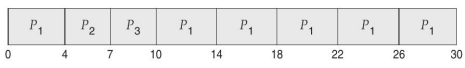
\includegraphics[width = .75\textwidth]{../res/imgs/CPU scheduling/RR.png}
    \caption{Diagramma di \textit{Gantt} dell'algoritmo RR.}
    \label{fig:RR}
\end{figure}
Osserviamo che il RR, per il processo $P_1$, ogni $q = 4$, si ferma per fare spazio agli altri processi mentre, per i processi $P_2$ e $P_3$, che durano meno di un quanto, quando terminano il Round Robin, non aspetta la scadenza del quanto per eseguire un altro processo ma comincia subito, che è un comportamento ragionevolmente ovvio. 
% 
\subsection{Reattività}
Cerchiamo ora di capire il vantaggio che forniscono gli algoritmi di scheduling preempitive (in particolare il RR) rispetto agli algoritmi non preemptive. Prendiamo come esempio i seguenti processi:
\begin{table}[h]
    \centering
    \begin{tabular}{c c}
        \textbf{Processo} & \textbf{Burst time} \\\hline
        $P_1$ & 6 \\
        $P_2$ & 3 \\
        $P_3$ & 1 \\\
        $P_4$ & 7 \\\hline
    \end{tabular}
\end{table}

\noindent Poniamo ora che il quanto di tempo \textit{q} sia 4. Calcoliamo ora il tournaround time medio tra questi processi: $P_1$ viene eseguti per 4 unità, dopo di chè viene fermato (gliene rimangono 2) e viene eseguito $P_2$ che terima ($T_{P_2}$ = 4 + 3 = 7); viene quindi eseguito $P_3$ che termina anche lui ($T_{P_3}$ = 7 + 1 = 8). A questo punto inizia l'esecuzione di $P_4$ che viene fermato dopo 4 unità (ne rimangono ancora 3) e viene fatto ripartire $P_1$ che termina ($T_{P_1}$ = 8 + 4 + 2 = 14) e infine viene fatto terminare anche $P_4$ ($T_{P_4}$ = 14 + 3 = 17). Per trovare il turnaround time medio si effettua la media dei 4 tournaround trovati.
\begin{gather*}
    \langle T \rangle = \frac{ T_{P_1} + T_{P_2} + T_{P_3} + T_{P_4}}{4} = \frac{14 + 7 + 8 + 17}{4} = \frac{46}{4} = 11.5
\end{gather*}

Osserviamo però che se avessimo utilizzato l'algoritmo SJF (vedi \ref{SJF}) il tournaround time medio è 8 che è minore rispetto a quello fornito da RR. Ciò significa che utilzzare un algoritmo pre-emptive, in termini di tempistiche, non è necessariamente la scelta migliore, è semplicemente un altro modo per schedulare l'esecuzione dei processi, ma non ne garantisce il miglioramento della prestazione. Allora perchè utilizzare questi algoritmo? Perchè migliora la reattività (\textbf{responsiveness}) del sistema. Ipotizziamo di avere un coda moltissimi processi che stanno in esecuzione. Un algoritmo non preempitve li esegue uno ad uno (secondo determinati criteri, più o meno efficienti) ma tutti i processi devono sempre stare in attesa che uno termini. Il RR invece garantisce che tutti i processi vengano eseguiti per almeno un certo quanto \textit{q} di tempo: è quindi un algoritmo più \textbf{equo} rispetto agli algoritmi non preemptive.

% 
\section{Scheduling con priorità} \label{priority scheduling}
Fino ad ora abbiamo trattato i processi in modo equo se non per la stima del \textit{burst time}. Introduciamo ora una seconda informazione, la \textbf{priorità} che non è altro che un numero che indica quanto sia importante (urgente) l'esecuzione di un determinato algoritmo. La priorità può essere sia legata al CPU burst time ma può anche essere legata ad altri aspetti. 

Arriva però un problema: la \textbf{starvation}. Anche in questo caso, come nel SRTF, può capitare che i processi che hanno una priorità di grado molto basso non vengano mai eseguiti in quanto sono sempre presenti processi con una priorità più alta. Con l'introduzione della priorità però, se un processo è da troppo tempo in coda, si aumenta di un grado la priorità al fine da mandarlo in esecuzione. Questa tecnica rappresenta allegoricamente l'invecchiamento (\textbf{aging}) del processo nella coda di attesa. 

Vediamo ora un primo esempio di scheduling con priorità puro. Abbiamo a che fare con i 5 processi seguenti:
\begin{table}[h]
    \centering
    \begin{tabular}{c c c}
        \textbf{Processo} & \textbf{Stima burst time} & \textbf{Priorità} \\\hline
        $P_1$ & 10 & 3 \\
        $P_2$ & 1 & 1 \\
        $P_3$ & 2 & 4 \\
        $P_4$ & 1 & 5 \\
        $P_5$ & 5 & 2 \\\hline
    \end{tabular}
\end{table}

\noindent Osserviamo che noi consideriamo come numero più basso la priorità più alta (di conseguenza $P_2$ è il processo con priorità più alta e $P_4$ quello con priorità più bassa). Detto ciò procediamo con il diagramma di Gantt (figura \ref{fig:priority_scheduling}).
\begin{figure}[h]
    \centering
    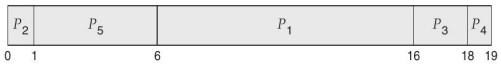
\includegraphics[width = .75\textwidth]{../res/imgs/CPU scheduling/priority_scheduling.png}
    \caption{Diagramma di \textit{Gantt} dell'algoritmo basato puramente sulla priorità.}
    \label{fig:priority_scheduling}
\end{figure}
Notiamo infatti che i processi sono eseguiti in ordine in base alla loro priorità: $P_2, P_5, P_1, P_3$ e $P_4$. Ovviamente, se durante l'esecuzione di $P_1$ (che ha priorità 3) fosse arrivato in coda un algoritmo con priorità 2, $P_1$ sarebbe stato interrotto per favorire l'esecuzione del nuovo processo. Inoltre, nel caso in cui due processi abbiano la stessa priorità si segue la dinamica FIFO, ovvero il primo processo che entra nella coda viene eseguito per primo rispetto ai processi con medesima priorità

% 
\subsection{Scheduling con prirità e RR}
Cerchiamo ora di raffinare un po' di più l'algoritmo fondendo la priorità con l'algoritmo di Round Robin. In particolare, nel momento in cui si hanno più processi che hanno lo stesso livello di priorità, al posto di seguire un approccio FIFO, si utilizza il Round Robin, garantendo quindi una maggiore reattività ai processi. Partiamo dal seguente set di processi:
\begin{table}[h]
    \centering
    \begin{tabular}{c c c}
        \textbf{Processo} & \textbf{Stima burst time} & \textbf{Priorità} \\\hline
        $P_1$ & 4 & 3 \\
        $P_2$ & 5 & 2 \\
        $P_3$ & 8 & 2 \\
        $P_4$ & 7 & 1 \\
        $P_5$ & 3 & 3 \\\hline
    \end{tabular}
\end{table}

\noindent Come è possibile osservare dalla figura \ref{fig:priority_RR}, notiamo che il processo 4, essendo che è l'unico processo con priorità 1, viene eseguito per primo e non viene interrotto da nessun'altro processo.
\begin{figure}[h]
    \centering
    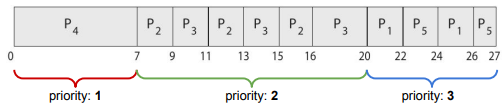
\includegraphics[width = .75\textwidth]{../res/imgs/CPU scheduling/priority_RR.png}
    \caption{Diagramma di \textit{Gantt} dello scheduling con priorità unito all'algoritmo RR per i processi con lo stesso grado di urgenza.}
    \label{fig:priority_RR}
\end{figure}
Dopo di che si effettua l'algoritmo RR con \textit{q} = 2 sui processi 2 e 3 in quanto hanno la stessa priorità. Infine, si fa lo stesso procedimento che con i processi 1 e 5 che hanno priortà 3. 

% 
\subsection{Coda multilivello}
\begin{wrapfigure}{o}{.25\textwidth}
  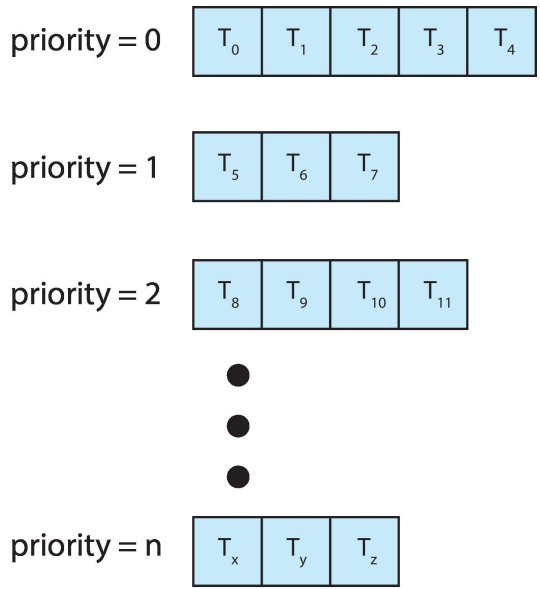
\includegraphics[width = \linewidth]{../res/imgs/CPU scheduling/multilevel_scheduling.png}
  \label{fig:multilevel_scheduling}
\end{wrapfigure}
Il fatto che per ogni grado di priorità venga eseguito il Round Robin ci porta a creare uno scheduling multilivello dove ogni livello corrisponde ad un grado di priorità. Di conseguenza nell'esecuzione viene prima eseguito il primo livello attraverso il RR; dopo di che si passa al secondo livello e così via fino all'ultimo grado di priorità. In particolare, le priorità più alte sono assegnati a processi che hanno un bisogno \textbf{real-time} (come per il controllo di un braccio robotico) che poi sono seguiti dai processi di sistema etc.

Questo ci porta al caso più complesso: immaginiamo che i processi non solo debbano essere inseriti nella coda giusta ma che questi debbano anche essere in grado di sposarsi da una coda all'altra e quindi cambiando il loro grado di priorità. Stiamo infatti parlando delle \textbf{Multilevel Feedback Queue} (MFQ).


% 
\section{Scheduling multiprocessore}
Fino ad ora abbiamo discusso di algoritmi tenendo conto del fatto che il sistema disponesse di un singolo processore; sappiamo bene però che nei sistemi moderni ormai una situazione del genere non si verifica più, con sistemi multicore. 

Come possono essere gestiti diversi threads all'interno di queste architetture multiprocessore? Nel caso del \textbf{Syimmetric multiprocessing} (SMP) 
\todo{Finisci introduzione CPU scheduling 2}

\subsection{Symmetric multiprocessing (SMP)}
Partiamo dalla situazione più semplice, nel casi in cui abbiamo a che fare con un'architettura SMP. In questo caso infatti abbiamo \textit{cores} che vengono gestiti in modo simmetrico (vedi paragrafo \ref{parallelismo}) e, disponendo di \textit{n} corse, l'unico problema da risolvere è come questi possano andare a gestire \textit{n} thread. Come è infatti possibile notare dalla figura \ref{fig:solutionAB}, un modo può essere quello di utilizzare una \textit{ready-queue} comune a tutti i cores oppure quello di creare una coda apposita ad ogni core per gestire i processi. 
\begin{figure}[h]
    \centering
    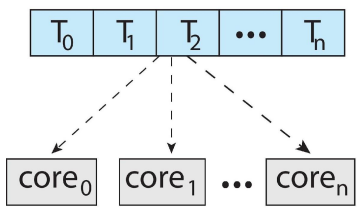
\includegraphics[width = .25\textwidth]{../res/imgs/CPU scheduling/solution_A.png}
    \hspace{2em}
    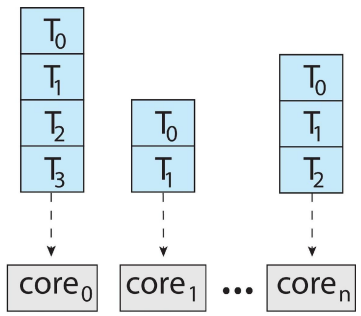
\includegraphics[width = .25\textwidth]{../res/imgs/CPU scheduling/solution_B.png}
    \caption{Ci sono diverse modi per gestire \textit{n} threads con \textit{n} cores.}
    \label{fig:solutionAB}
\end{figure}
Entrambe le soluzioni sono più che lecite anche se ad oggi i sistemi operativi moderni tendono ad usare la seconda in quanto la prima soluzione, essendo si che si ha a che fare con una coda condivisa è complicato gestire la condivisione di tale risorsa tra i cores (problemi di \textit{race conditions}).

\subsection{}
% minuto 7:50 di Lez. 16-03


















% Solution A - Solution B - memory stall - memory stall 2 - two levels scheduling


\section{Scheduling real-time}
\section{Valutazione di un algoritmo}

\todo{Finisci CPU scheduling: parte 2}


\newpage\part{Sincronizzazione dei Processi}

\pagebreak
\section{Sincronizzazione}\label{sincronizzazione}
Come abbiamo visto nel capitolo \ref{processes},i processi possono essere eseguiti sia in parallelo che in concorrenza, la quale non è altro che un modo per far apparentemente girare due processo in maniera parallela quando in realtà stanno condividendo lo stesso \textit{core} del sistema. Un processo può quindi essere interrotto in qualunque momento da un algoritmo di scheduling (come il \textit{Round Robin}) per fare spazio ad un altro processo. Cosa succede però se viene interrotto in un momento in cui sta accedendo nella memoria condivisa con un altro processo e, lasciando spazio all'altro, vengono modificati dei dati? Capiremo, in questa sezione, che l'obiettivo da raggiungere è quindi la \textbf{cooperazione} tra processi in modo tale che non si verifichino situazioni spiacevoli.

\subsection{Sezione critica}
Poniamo ora di avere a che fare con due processi i quali effettuano due \texttt{fork} simultanei (figura \ref{fig:sim_fork_issue}).
\begin{figure}[!h]
    \centering
    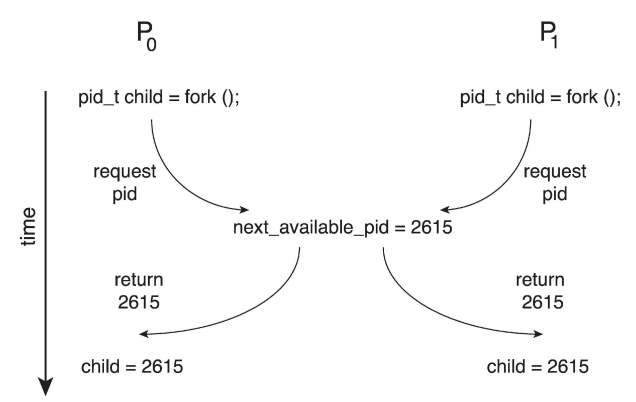
\includegraphics[width=.5\textwidth]{../res/imgs/synchronization/sim_fork_issue.png}
    \caption{Creazione di due processi figli con lo stesso \texttt{PID}.}
    \label{fig:sim_fork_issue}
\end{figure}
Supponiamo di avere una variabile, chiamata \texttt{next\_available\_pid} che contiene il primo \texttt{PID} disponibile. Se i due processi, in questo caso $P_0$ e $P_1$, fanno accesso alla variabile in maniera simultanea, verranno creati due figli con lo stesso \texttt{PID}. I due processi hanno fatto un accesso in maniera non esclusiva alla stessa zona di memoria condivisa generando quindi un problema.

Quello che abbiamo appena visto non è altro che un esempio di \textbf{critical section problem}. Generalizzando, possiamo dire che ogni processo è composto di un segmento di codice che deve avere un \textbf{accesso esclusivo} in quanto ha un accesso in scrittura dove aggiorna tabelle, modifica variabili o scrive su files. Di conseguenza si cerca di non interrompere un processo nel momento in cui questo è nella sua \textbf{sezione critica}.
% 
\subsubsection{Requisiti}\label{CS requisiti}
È stato stilato un elenco di 3 punti di requisiti che devono essere rispettati affinché non vengano generate situazioni dove un processo viene interrotto durante la sua sezione critica.
\begin{enumerate}
    \item \textbf{Mutua esclusione}: se il processo $P$ sta eseguendo la sua parte critica nessun altro processo deve interromperlo;
    \item \textbf{Progresso}: bisogna garantire che nessun processo rimanga in un'attesa perenne mentre aspetta la conclusione della parte critica di un altro processo. In altre parole, l'esecuzione della sezione critica di un processo non può essere posticipata in maniere indeterminata;
    \item \textbf{Attesa limitata}: deve esistere un limite massimo per cui un processo deve concludere la sua parte critica. 
\end{enumerate}
% 
\subsubsection{Soluzioni inefficienti}
Una prima idea banale è quella di \textbf{disabilitare} gli \textbf{interrupt} nel momento in cui un processo (un \textit{thread}) sta eseguendo la sua parte critica. Questa però è una soluzione poco elegante e anche poco funzionale. Si rischia infatti di far aspettare molto altri processi i quali necessitano di eseguire la loro sezione critica (starvation). 

Si è quindi pensato ad una soluzione un po' più elegante, ma che comunque è una forma embrionale rispetto a ciò che vedremo. Stiamo parlando di una semplice \textbf{soluzione software} tra due processi dove entrambi condividono una variabile \textit{booleana} \texttt{turn} che indica di chi è il turno per eseguire la sezione critica.
\begin{lstlisting}
while(true){
    while(turn == j); /* attendo che sia il mio turno */
    /* SEZIONE CRITICA */
    turn = j; /* rimando il turno all'altro processo */
    /* sezione rimasta */
}
\end{lstlisting}
Con questa soluzione, è rispettata la richiesta di mutua esclusione ma i punti (2) e (3) non sono rispettati: il processo \texttt{j} potrebbe anche durare un'ora e ci sarebbe un'ora di attesa. Non sono quindi i rispettati i limiti di attesa e nemmeno il progresso dei processi.
% 
\subsection{Soluzione di Peterson}
Una prima soluzione un po' più raffinata è quella di Peterson. In questa soluzione i due processi condividono due variabili:
\vspace{-5px}
\begin{itemize}
\setlength{\itemsep}{-.15 em}
    \item \texttt{turn} che è la variabile che indica di quale processo è il turno;
    \item \texttt{flag[2]} che è un array di due valori booleani che indicano se il processo i-esimo è pronto o meno per entrare nella sezione critica.
\end{itemize}

Come possiamo notare dal seguente segmento di codice, sono stati aggiunti alcuni controlli.
\begin{lstlisting}[caption={Soluzione di Peterson}]
while (true){
    flag[i] = true;
    turn = j;
    while (flag[j] && turn == j); /* aspetto fino a che non sono pronto e fino a che j non ha finito */
    /* SEZIONE CRITICA */
        flag[i] = false;
    /* sezione rimasta */
}
\end{lstlisting}
Osserviamo che possiamo intendere l'esecuzione della parte critica di un processo come una galleria a senso unico alternato: se un processo deve entrarci ma al suo interno ce n'è già un altro attende, altrimenti ci entra. L'esecuzione in "parallelo" è quindi mantenuta dato che un processo può essere molto lontano dalla galleria mentre il secondo la sta attraversando. Con questo modello, quindi, tutti e 3 i requisiti sono rispettati.
% 
\subsubsection{Architetture moderne}
Ciò nonostante, questa soluzione diventa obsoleta per i sistemi moderni \textit{multicore} e \textit{multithread}. Questo perché nelle architetture moderne il compilatore si prende la libertà di riordinare e riorganizzare il codice. Vediamo un esempio di due thread (assumiamo che le variabile condivise siano \texttt{x} e \texttt{flag}):
\begin{lstlisting}
/* THREAD 1 */
    while(!flag);
    print x

/* THREAD 2 */
    x = 100;
    flag = true;
\end{lstlisting}
Una volta eseguito il codice, ci aspettiamo che l'output sia \texttt{100}. Però, se le istruzioni nel thread 2 vengono invertite, il risultato è completamente diverso, perché il thread 1 viene eseguito prima che la variabile \texttt{x} venga cambiata a 100.
\begin{lstlisting}
/* THREAD 2 */
    flag = true;
    x = 100;
\end{lstlisting}

Al fine di fare in modo che la soluzione di Peterson funzioni anche nelle architetture moderne si introduce la \textbf{memory barrier}: questa è un'istruzione che rende le modifiche effettuate in memoria visibili a tutti i processori (\textit{cores}). Questo tipo di modello di memoria si dice \textit{strongly ordered}, ovvero una modifica in memoria è propagata immediatamente a tutti i core; si contrappone al \textit{weakly ordered} dove una modifica in memoria non è propagata istantaneamente. 

Con l'introduzione delle memory barrier ora la soluzione di Peterson rimane valida. Questo perché quando viene invocato un \texttt{memory\_barrier()} il sistema si assicura che tutti i load e store in memoria vengano completati prima di ogni altro load e store. Quindi anche se il codice venisse riordinato, la memory barrier si assicura che le modifiche in memoria siano completate. 
% 
\subsection{Sincronizzazione via hardware}
Tra le diverse soluzioni che abbiamo visto, la più gettonata rimane comunque l'implementazione di particolari \textbf{istruzioni hardware} che permettono di modificare il contenuto di una \textit{word} in memoria oppure di effettuare uno \textit{swap} di due word.

\subsubsection{Test and set}
La prima delle due istruzioni HW che discuteremo è la \texttt{test\_and\_set} dove prende un input booleano e lo memorizza in una variabile temporanea \texttt{tmp}; in secondo luogo il valore in ingresso viene settato a \texttt{true} e infine la variabile temporanea viene restituita. Lo pseoudcodice di quest istruzione è il seguente (ricordiamo che sono istruzioni a livello HW, quindi il codice è solo a scopo concettuale):
\begin{lstlisting}
boolean test_and_set(boolean *target){
    boolean tmp = *target;  /* salvo il valore di target */ 
    *target = true; /* setto a TRUE */
    return tmp;
}
\end{lstlisting}
Si osserva che dopo l'esecuzione dell'istruzione, il valore di \texttt{target} è sempre \texttt{true} e viene ritornato il vecchio valore della variabile in ingresso. Ricordiamo infine che è un'istruzione \textbf{atomica}, ciò significa che non può essere interrotta.

Vediamo ora come questa istruzione posso esserci utile per l'esecuzione della sezione critica di un processo:
\begin{lstlisting}[caption={Utilizzo \texttt{test\_and\_set}}]
while(true){
    while(test_and_set(&lock)); /* lock = true, attendo per la risolrsa, ora e' occupato.*/
        /* lock = false, posso cominciare a eseguire la parte critica perche' si e' liberato; metto lock = true*/
    /* SEZIONE CRITICA */
    lock = false; /* lock e' libero */ 
    /* sezione rimanente */
}
\end{lstlisting}
% 
\subsubsection{Compare and swap}
La seconda istruzione HW che andiamo a discutere si chiama \texttt{compare\_and\_swap} e, come per la precedente, anch'essa è un'istruzione atomica. Come vedremo, questa istruzione, ha ben 3 variabili in ingresso:
\vspace{-5px}
\begin{itemize}
\setlength{\itemsep}{-.15 em}
    \item \texttt{value}, che indica il valore da modificare;
    \item \texttt{expected}, che indica il valore che ci si aspetta contenga \texttt{value};
    \item \texttt{new\_value}, ovvero il nuovo valore con cui vogliamo cambiare \texttt{value}.
\end{itemize}
Osserviamo ora lo pseudocodice dell'istruzione:
\begin{lstlisting}
int compare_and_swap(int *value, int expected, int new_value){
    int tmp = *value;
    if (*value == expected)
        *value = new_value;
    return temp; /* ritorna vecchio valore di value */
}
\end{lstlisting}
Notiamo che, a differenza di \texttt{test\_and\_set}, in questo caso il valore di \texttt{value} viene modificato solo nel momento in cui coincide con il valore che ci aspettiamo questo viene modificato con il valore inserito (\texttt{new\_value}). Capiamo ora come questa istruzione possa essere utilizzata per la gestione della sezione critica e come questa sia più \textbf{flessibile} rispetto alla precedente.
\begin{lstlisting}[caption={Utilizzo di \texttt{compare\_and\_swap}}]
while(true){
    while(compare_and_swap(&lock, 0, 1) != 0); 
        /* lock = 1 = true, continuo ad aspettare */
        /* lock = 0 = false, viene ritornato 0, quindi esco dal while, e occupo lo spazio, lock = 1 */
    /* SEZIONE CRITICA */
    lock = 0;
    /* sezione rimasta*/
}
\end{lstlisting}

% 
\subsubsection{Variabili atomiche}
Istruzioni come \texttt{compare\_and\_swap} sono utilizzate per comporre dei blocchi per comporre altri oggetti di sincronizzazione. Uno tra questi oggetti è la variabile atomica che fornisce degli aggiornamenti elementare a dei dati primitivi. Segue infatti l'esempio di \texttt{increment()} dove il valore intero \texttt{v} viene incrementato senza interruzioni
\begin{lstlisting}[caption={Esempio di una variabile atomica \texttt{increment()}}]
void increment(atomic_int *v){
    int temp;
    do{
        temp = *v;
    } while (temp != compare_and_swap(v, temp, temp+1));
}
\end{lstlisting}
% 
\subsection{Mutex lock e Semafori}
Le soluzioni che abbiamo visto in precedenza erano intricate e spesso non erano accessibili da applicazioni esterni; inoltre creano ulteriori complicazioni in sistemi multithreading. A questo proposito i progettisti di sistemi operativi hanno costruito diversi \textit{tool} al fine di risolvere il problema della sezione critica.

Il primo che andremo a vedere è il \textbf{mutex lock} (\textbf{MUT}ual \textbf{EX}clusion lock) che è una variabile booleana che indica se il \textbf{lock}, ovvero la sezione critica è disponibile o meno. Questa è protetta da due istruzioni atomiche di acquisizione e rilascio:
\vspace{-5px}
\begin{itemize}
\setlength{\itemsep}{-.15 em}
    \item \texttt{acquire()} che blocca la \textit{CS}\footnote{\textit{CS} sta per \textit{Critic Session}, ovvero sezione critica};
    \item \texttt{release()} che rilascia il lucchetto e quindi la \textit{CS} è liberata.
\end{itemize}
Spesso queste sono implementate via HW attraverso istruzioni come \texttt{compare\_and\_ swap}.

Come possiamo notare dallo pseudocidce sottostante, ci troviamo in una situazione di \textbf{busy waiting} in quanto il thread continua ad entrare nel ciclo fino a che non acquisisce il lucchetto. È evidente che stiamo sprecando CPU, che potrebbe essere usata per altri thread.
\begin{lstlisting}
while(true){
    acquire();
    /* SEZIONE CRITICA */
    release();
    /* sezione rimanente */
}
\end{lstlisting}

A questo proposito, questa pratica è raffinata tramite i \textbf{semafori}, che non sono altro che una \textbf{variabile intera} (\texttt{S}) accessibile, anche in questo caso attraverso due operazioni atomiche: \texttt{wait()} e \texttt{signal()}.
\begin{lstlisting}
wait(S){
    while (S<=0); /* busy wait */
    S--;
}

signal(S){
    S++;
}
\end{lstlisting}
Se la variabile \texttt{S} può assumere solo il valore di 0 o 1, si parla di semafori \textbf{binari} (ovvero dei mutex lock), altrimenti si fa riferimento ai \textbf{counting semaphores}. 

Attraverso i semafori abbiamo la possibilità di fare eseguire una parte di processo prima che un altro processo inizi. Siano $P_1$ e $P_2$ due processi che contengono il segmento $S_1$ ed $S_2$; per fare in modo che $S_1$ sia eseguito prima di $S_2$ possiamo utilizzare i semafori.
\begin{lstlisting}
P1:
    S1;     /* eseguo S1 */
    signal(synch); /* dico a P2 che ho finito */

P2:
    /* busy wait */
    wait(synch); /* aspetto che P1 abbia finito */
    S2;     /* eseguo S2 */
\end{lstlisting}
Possiamo notare però che anche in questo caso $P_2$ è in una fase di busy waiting.

\subsubsection{Waiting queue}
Per evitare che accada è necessario implementare una \textbf{waiting queue}:
\begin{lstlisting}[caption={Struttura del semaforo con waiting queue}]
typedef struct {
    int value;
    struct process *list;   /* indica la prossima entry nella lista */
} semaphore
\end{lstlisting}
Qui abbiamo a disposizione altre due operazioni per implementare la sincronizzazione tra processi:
\vspace{-5px}
\begin{itemize}
\setlength{\itemsep}{-.15 em}
    \item \texttt{sleep()} che mette a dormire il processo o il thread e lo inserisce nella waiting queue;
    \item \texttt{wakeup()} che rimuove il primo processo della coda e lo inserisce nella \textit{ready queue}, coda che contiene i processi pronti per essere eseguiti.
\end{itemize}

A questo punto possiamo ridefinire le due operazioni basi del semaforo: \texttt{wait} e \texttt{signal}.
\begin{lstlisting}[caption={Utilizzo di semaforo con \textit{waiting queue}}]
wait(semaphore *s){
    S->value--;     /* decremento il valore del semaforo */
    if (S->value < 0){
        aggiungi processo in S->list;
        sleep();    /* evito il busy waiting, mi tolgo dalla CPU e aspetto che signal() mi svegli dalla coda */
    }
}

signal(semaphore *S){
    S->value++;     /* incremento il valore del semaforo */
    if (S->value <= 0){
        rimuovii processo in S->list;
        wakeup();
    }
}
\end{lstlisting}

Bisogna però fare attenzione a utilizzare \texttt{wait} e \texttt{signal} nel modo corretto: non si può prima invocare \texttt{signal} e poi \texttt{wait} oppure invocare \texttt{wait} due volte di seguito. Questo utilizzo incorretto delle due operazioni può generare errori.
% 
\subsection{Monitor}
Cerchiamo ora di risolvere il problema dei semafori: le operazioni di \texttt{wait} e \texttt{signal} erano lasciate al programmatore. Questa scelta ha come unica conseguenza la generazione di errori da parte dell'utilizzatore (che, come vedremo più avanti prendono il nome di \textbf{deadlock}, capitolo \ref{deadlocks}). Cerchiamo quindi di implementare un'astrazione dei semafori al fine di limitarne i danni. Queste astrazioni di alto livello sono proprio i \textbf{monitor} i quali garantiscono l'esecuzione di un processo alla volta.

\subsubsection{Struttura e implementazione}
La struttura di astrazione del monitor è formata da una variabile condivisa da tutti i processi, da del codice di inizializzazione per il monitor e da tante funzioni o procedure (ogni processo ha le stesse procedure).
\begin{lstlisting}[caption={Struttura del monitor}]
monitor name{
    /* dichiarazione della variabile condivisa */
    codice di inizializzazione (...) { ... }

    procedura F1 (...) { ... }
    procedura F2 (...) { ... }
    /* ... */ 
    procedura Fn (...) { ... }    
}
\end{lstlisting}
Come possiamo osservare dalla figura \ref{fig:monitor}, concettualmente, il monitor raggruppa tutti i processi attraverso dei dati condivisi in una coda.
\begin{figure}[!h]
    \centering
    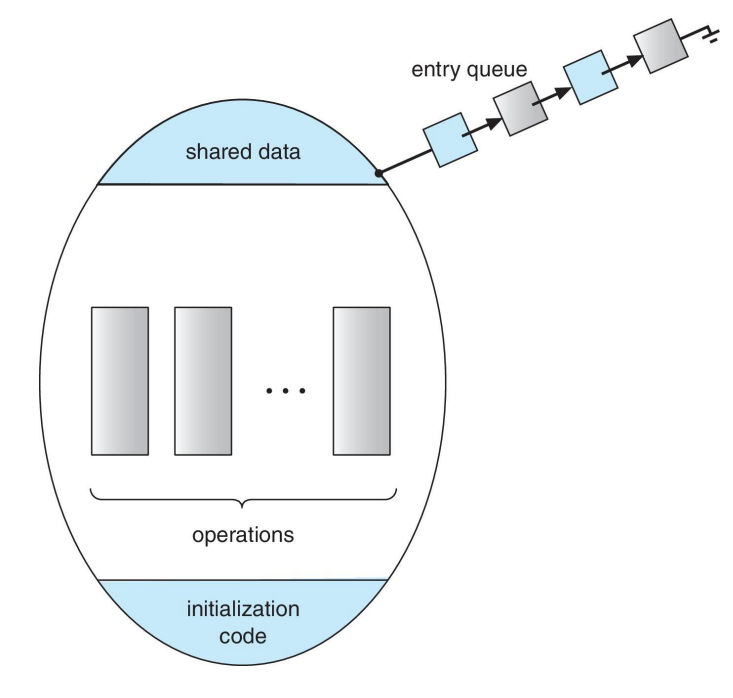
\includegraphics[width=.55\textwidth]{../res/imgs/synchronization/monitor.png}
    \caption{La struttura di astrazione del monitor.}
    \label{fig:monitor}
\end{figure}

Per implementare un monitor ci appoggiamo sui semafori, in particolare su un mutex:
\begin{lstlisting}
semaphore mutex = 1;    /* semaforo binario = mutex */

wait(mutex) /* aspetto che il mutex si liberi per occuparlo */
    /* corpo della funzione Fi */
signal(mutex) /* libero il mutex **/
\end{lstlisting}
È quindi necessario modificare ogni procedura del monitor bloccando e poi rilasciando il mutex. In questo modo, a differenza dei semafori, le operazioni di \texttt{wait} e \texttt{signal} sono già implementate all'interno delle procedure che eseguono quelle operazioni, al posto del programmatore. Un esempio di utilizzo completo è presente nella sezione \ref{utilizzo monitor}.

\subsubsection{Variabile di condizione}
Oltre alla struttura base, illustrata nel paragrafo precedente, possiamo anche inserire le \textit{condition variables}  (rappresentazione in figura \ref{fig:condition_variable}) che possono eseguire le stesse due operazioni dei semafori: \texttt{wait} e \texttt{signal}.
\begin{figure}[!h]
    \centering
    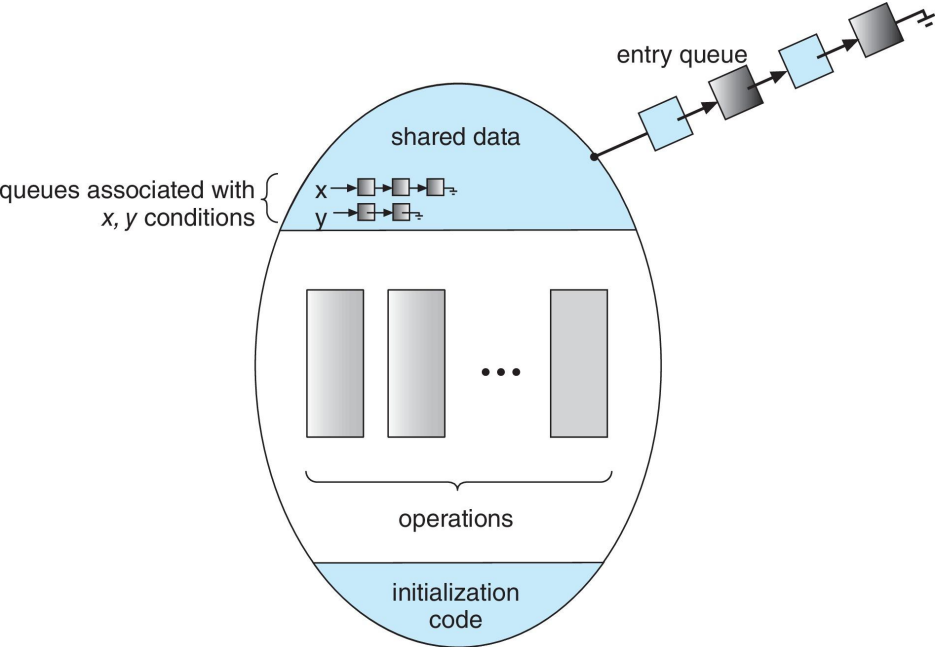
\includegraphics[width = .65\textwidth]{../res/imgs/synchronization/condition_variable.png}
    \caption{Caption}
    \label{fig:condition_variable}
\end{figure}
In questo caso però le due operazioni sono modificate e non portano ad errori se utilizzate male. Ricordiamo che, nel caso dei semafori, se \texttt{signal} fosse stato invocato senza aver prima invocato il corrispettivo \texttt{wait}, avrebbe erroneamente incrementato il contatore. In questo caso invece, se non è presente alcun processo in \texttt{wait}, allora \texttt{signal} non fa nulla.

Emerge ora un piccolo dubbio. Se ci sono diversi processi che sono in \texttt{wait}, quando viene effettuato un \texttt{x.signal()}, quale di questi processi viene eseguito per prima? Notiamo che ci troviamo in una situazione molto simile allo scheduling (capitolo \ref{CPU scheduling}) solo che, in questo caso non è più a livello di sistema operativo ma è a livello di monitor e di accesso alla sezione critica. Per risolvere questo problema ci possono essere algoritmi come FCFS oppure a livello di priorità: chi ha la priorità più alta viene fatto eseguire prima. Spesso la priorità è definita in base al tempo di utilizzo della sezione critica, ma si fa presente che se entrano nella coda processi con un tempo di utilizzo molto breve, i processi con un utilizzo lungo possono essere in attesa perenne ed andare in \textbf{stravation}. Ecco che non viene più rispettato il terzo requisito, ovvero che l'attesa di un processo per la sezione critica deve essere limitata (vedi paragrafo \ref{CS requisiti}).
% 
\subsection{Problemi comuni della sincronizzazione}


\subsubsection{Buffer limitato}
Il primo problema che andiamo a discutere è il problema del buffer limitato. Abbiamo a disposizione un buffer che contiene \textit{n} elementi, ovvero il numero di processi in coda per accedere alla loro sezione critica. Disponiamo inoltre di tre semafori:
\vspace{-5px}
\begin{itemize}
\setlength{\itemsep}{-.15 em}
    \item \texttt{mutex} che consente l'accesso al buffer in maniera esclusiva (inizializzato ad 1);
    \item \texttt{full} che segnala in numero di elementi contenuti all'interno del buffer (inizializzato a 0);
    \item \texttt{empty} che indica la quantità di spazi disponibili all'interno del buffer, sarebbe \textit{n - }\texttt{full} (inizializzato ad \textit{n}).
\end{itemize}
Analizziamo la soluzione del problema, che è molto simile al problema del produttore e consumatore.
\begin{lstlisting}[caption = {Problema del buffer limitato}]
/* Produttore */
while (true){
    /* produco un elemento */
    wait(empty); /* aspetto che ci sia spazio all'interno del buffer, ovvero che ci sia almeno una locazione libera (empty > 0) */
    wait(mutex); /* ora che c'e' un posto libero, richiedo l'accesso alla sezione critica */
    /* SEZIONE CRITICA: aggiungo il codice nel buffer */
    signal(mutex); /* libero la sezione critica */
    signal(full); /* incremento di 1 il numero di elementi nel buffer
}

/* Consumatore */
while(true){
    wait(full); /* aspetto che ci siano >0 elementi nel buffer */
    wait(mutex); /* aspetto l'accesso esclusivo nel buffer */
    /* SEZIONE CRITICA: rimuovo l'elemento dal buffer */
    signal(mutex); /* libero la sezione critica */
    signal(empty); /* incremento il numero di locazioni libere */
}
\end{lstlisting}

Osserviamo che i comando \texttt{wait(empty)} e \texttt{wait(mutex)} all'interno di produttore \textbf{non} possono essere invertiti. Se prima infatti viene bloccato il mutex, il consumatore non sarà più in grado di liberare il buffer che, se è pieno, porta ad un'attesa perenne il produttore in \texttt{wait(empty)}: siamo ricaduti in una situazione di \textit{deadlock}.

% 
\subsubsection{Problema dei lettori e degli scrittori}
Il secondo problema è detto dei lettori e degli scrittori. In questo caso: (1) più lettori possono leggere lo stesso dataset (che può essere anche un file su disco) contemporaneamente (per definizione, non possono modificarlo) e (2) lo scritture deve poter scrivere sul dataset senza che quest'ultimo venga letto. Solo nel momento in cui ha terminato (mutua esclusione), allora i lettori possono effettuare nuovamente l'accesso simultaneo. 

Non ci soffermiamo sul codice, ci limitiamo a dire che è sufficiente utilizzare due semafori:
\vspace{-5px}
\begin{itemize}
\setlength{\itemsep}{-.25 em}
    \item \texttt{rw\_mutex}, semaforo binario inizializzato ad 1, che indica che la risorsa è occupata dallo scrittore;
    \item \texttt{mutex}, anch'esso un semaforo binario che segnala che la risorsa è in lettura da almeno un lettore;
    \item \texttt{read\_count}, un intero che conta il numero di lettore che stanno leggendo la risorsa.
\end{itemize}

In questo caso i problemi generati sono due. Il primo è che c'è la possibilità che lo scrittore non riesce mai ad effettuare l'accesso, entra quindi in una fase di attesa perenne. Il secondo problema che emerge è che quando lo scrittore ha effettuato l'accesso, nessun lettore è in grado di accedere: anche in questo caso si può ricadere in una fase di \textit{starvation}.

% 
\subsubsection{Problema dei 5 filosofi}\label{5_filosofi}
Il problema dei 5 filosofi, rimane il più conosciuto (e il più importante).
\begin{figure}[t!]
    \centering
    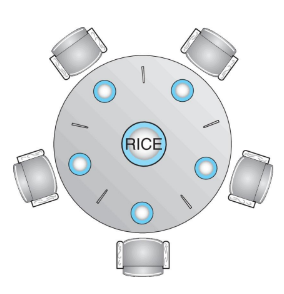
\includegraphics[width = .5\textwidth]{../res/imgs/synchronization/5_filosofi.png}
    \caption{Disposizione dei 5 filosofi.}
    \label{fig:5_filosofi}
\end{figure}
Un filosofo, può pensare o mangiare. Facendo riferimento alla figura \ref{fig:5_filosofi}, osserviamo che i filosofi sono disposti in un tavolo rotondo che ha al centro una scodella di riso (che allegoricamente indica il dataset, ovvero la risorsa condivisa). Alla destra e alla sinistra di ciascun filosofo è presente una bacchetta: questa rappresenta il semaforo in quanto se un filosofo smette di pensare e inizia a mangiare, non può farlo se il filosofo alla sua sinistra o alla sua destra sta mangiando, in quanto almeno una delle due bacchette sono occupate.

Proviamo a dare una prima soluzione a questo problema di sincronizzazione con i semafori. 
\begin{lstlisting}[caption = {Risoluzione del problema dei  filosofi con i semafori}]
while(true){
    wait(chopstick[i]); /* attende la bacchetta a sinistra */
    wait(chopstick[ (i + 1) % 5]); /* attende la bacchetta a destra */
    /* SEZIONE CRITICA: mangia dalla ciotola di riso */
    signal(chopstick[i]); /* rilascia la bacchetta a sx */
    signal(chopstick[ (i + 1) % 5]); /* rilascia la bacchetta a dx */
    /* pensa */
}
\end{lstlisting}
Sembrerebbe tutto ottimo, ma cosa succede se tutti e 5 i filosofi prendono la loro bacchetto sinistra allo stesso tempo? Entrano in una situazione di attesa infinita (deadlock) un quanto tutte le loro bacchette destre sono occupate dal filosofo alla loro destra. Proviamo a risolvere questo nuovo problema attraverso i \textbf{monitor}.\label{utilizzo monitor}
\begin{lstlisting}[caption = {Risoluzione del problema dei  filosofi con i monitor}]
monitor DiningPhilosophers{  /* creo la struttura astratta */
    enum { THINKING, HUNGRY, EATING } state[5]; /* per ogni filosofo e' definito lo stato in cui si trova */
    condition self[5];  /* condition variable */

    void test(int i){
        if ((state[(i + 4) % 5] != EATING) /* se il vicino di sinistra non sta mangiano */ &&
            (state[i] == HUNGRY) /* se ho fame */ &&
            (state[(i + 1) % 5] != EATING)) /* se il vicino di destra non sta mangiando */ {
                state[i] = EATING; /* mi metto a mangiare */
                self[i].signal();
            }
    }

    void pickup(int i){ /* acquire */
        state[i]  = HUNGRY;
        test(i); /* se posso, mi metto a mangiare */
        if (state[i] != EATING) /* se non sto mangiando */
            self[i].wait(); /* mi metto in attesa*/
    }

    void putdown(int i){ /* release */
        state[i] = THINKING; /* mi rimetto a pensare */
        /* controllo che il mio vicino sinistro e destro non siano in attesa */
        test((i + 4) % 5);
        test((i + 1) % 5);
    }

    initialization_code(){ /* all'inizio tutti i filosofi stanno pensando */
        for (int i = 0; i < 5; i++)
            state[i] = THINKING; 
    }
}

\end{lstlisting}
Dopo aver implementato questa struttura astratta è semplicemente necessario utilizzare le due operazione \texttt{pickup()} e \texttt{putdown()} al fine di fare in modo che tutti i filosofi mangino sincronizzati. Ad ogni modo, anche in una situazione così raffinata la \textbf{starvation} è possibile, nel caso in cui un filosofo si metta a mangiare e non smetta più.
\begin{lstlisting}
DiningPhilosophers.pickup(i);
    /* SEZIONE CRITICA (mangio) */
DiningPhilosophers.putdown(i);
\end{lstlisting}


\pagebreak
\chapter{Deadlocks} \label{deadlocks}
In questo capitolo cercheremo di approfondire i deadlocks: capiremo sotto quali condizioni si giungerà ad una soluzione di deadlock e i diversi algoritmi per la gestione dei deadlocks.

\subsubsection*{Modello di sistema}
Prima di discutere effettivamente dei deadlock è importante fare un piccola premessa. In questo capitolo avremo a che fare con sistemi che possono essere composti da \textit{m} tipi di risorse generiche: queste potrebbero essere dei dispositivi I/O, dati su disco, delle allocazioni in memoria, la CPU oppre dei semafori generici. Queste risorse vengono definite con la notazione $R_m$. Inoltre, ogni tipo di risorsa può essere \textbf{singolo}, come un slot del DVD sul computer, oppure \textbf{multiplo} come la presenza di diverse porte USB oppure molti buffer in memoria.
% 
\section{Nozioni fondamentali}
Ripassiamo innanzitutto il concetto di deadlock. Prendiamo il caso in cui due semafori $S_1$ ed $S_2$, entrambi inizializzati a 1, siano condivisi da due thread $T_1$ e $T_2$. Osservando lo pseudo-codice seguente, si ha una classica situazione di deadlock. Se $T_1$ e $T_2$ sono eseguiti contemporaneamente, $T_1$ occupa subito $S_1$ e $T_2$ occupa subito $S_2$. Dopo di che $T_1$ aspetta $S_2$ che però è occupato da $T_1$ il quale è in attesa di $S_1$, occupato da $T_1$. Siamo quindi in una situazione di stallo dove entrambi i thread stanno aspettando l'altro e nessuno dei due termina l'esecuzione

\begin{lstlisting}[caption = {Classica situazione di deadlock}]
/* T1 */
    wait(S1); /* occupa S1 */
    wait(S2); /* aspetta per S2 */

/* T2 */
    wait(S2); /* occupa S2 */
    wait(S1); /* attende S1 */
\end{lstlisting}
% 

% 
\subsection{Caratterizzazione}\label{4_punti_deadlock}
Possiamo osservare che si devono verificare 4 condizioni affinché si arrivi ad una situazione di deadlock.
\vspace{-5px}
\begin{enumerate}
    \setlength{\itemsep}{-.15 em}
    \item \textbf{Mutua esclusione}: banalmente, ci deve essere almeno una risorsa che sia utilizzata da un thread alla volta;
    \item \textbf{Hold and wait}: deve esistere almeno un thread che sta cercando di accedere alla risorsa che è già occupata e, di conseguenza, deve attendere;
    \item \textbf{No preemption}: una risorsa può essere rilasciata volontariamente dei thread. Le risorse non possono quindi essere "rubate" da altri thread e, di conseguenza, un thread non può essere spezzato durante la sua fase critica;
    \item \textbf{Attesa circolare}: è il requisito più importante, deve verificarsi una situazione come quella dei cinque filosofi (paragrafo \ref{5_filosofi}), ovvero che un thread attende la conclusione di un altro thread che ... che aspetta la conclusione del thread iniziale.
\end{enumerate}
Se almeno una di queste quattro condizioni \textbf{non} è \textbf{verificata} allora non si è in una situazione di deadlock.

% 
\subsection{Grafo risorsa-allocazione}
Uno strumento molto importante, utile per visionare i diversi casi di deadlock è il grafo risorsa-allocazione. Questo grafo è composto, come ogni grafo, da vertici e archi. I vertici si suddividono in due tipi: il primo tipo rappresenta la risorsa $R_m$ mentre il secondo tipo indica il thread $T_n$. Il grafo è \textbf{diretto}, ciò significa che gli archi hanno una direzione. In particolare $R \to T$ indica che il thread $T$ detiene/occupa la risorsa $R$, mentre $T \to R$ segnala che il thread $T$ è in attesa della risorsa $R$. Inoltre, si osserva che generalmente i vertici che rappresentano una risorsa multipla contengono tanti pallini ($\bullet$) quante sono le istanze di quella risorsa disponibili (come le 5 porte USB). 

Prendiamo come esempio la figura \ref{fig:grafo_deadlock}. Possiamo notare che rispetta tutte "regole" del grafo risorsa-allocazione. In particolare possiamo affermare che $R_1$ ed $R_3$ sono risorse singole mentre $R_2$ ed $R_4$ sono risorse multiple (con, rispettivamente, 2 e 4 istanze).
\begin{figure}[h]
    \centering
    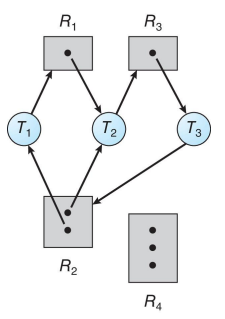
\includegraphics[width = .35 \textwidth]{../res/imgs/deadlocks/deadlock_graph.png}
    \caption{Rappresentazione grafica di un grafo che presenta una situazione di deadlock.}
    \label{fig:grafo_deadlock}
\end{figure}
Inoltre possiamo dire che ci troviamo in una situazione di \textit{deadlock}. Perché? Partiamo da $R_2$, questa è occupata da $T_1$ e $T_2$; $T_1$ è in attesa di $R_1$ la quale è occupate da $R_2$ che, a sua volta, sta aspettando che $R_3$ venga liberata da $T_3$ il quale sta attendendo la liberazione due $R_2$, occupata per l'appunto da $T_1$ e $T_2$. È proprio una situazione di deadlock: a primo impatto possiamo dire ciò perché è presente un \textbf{ciclo}. Osservando però la figura \ref{fig:grafo_no_deadlock}, capiamo che il fatto che ci sia un ciclo non implica che ci sia per forza una situazione di deadlock.
\begin{figure}[h]
    \centering
    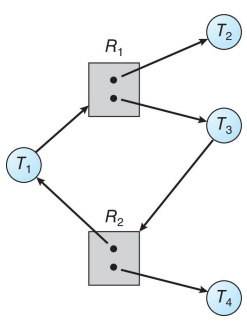
\includegraphics[width = .35\textwidth]{../res/imgs/deadlocks/no_deadlock_graph.png}
    \caption{Rappresentazione grafica di un grafo senza deadlock.}
    \label{fig:grafo_no_deadlock}
\end{figure}
Se osserviamo infatti la figura \ref{fig:grafo_no_deadlock} riconosciamo che prima o poi il thread $T_2$ oppure $T_4$ rilascerà la risorsa e di conseguenza le richiesta degli altri thread saranno soddisfatte.

Riassumiamo ora queste informazioni nel seguente diagramma: 
\begin{figure}[h]
    \centering

    \begin{tikzpicture}
  [
    grow                    = down,
    sibling distance        = 10em,
    level distance          = 6em,
    edge from parent/.style = {draw, -latex},
    every node/.style       = {font=\footnotesize},
    sloped
  ]
  \node [root] {Contiene cicli?}
    child { node [env] {Non ci sono\\deadlock.}
      edge from parent node [above] {No} }
    child { node [env] {Ci sono\\solo risorse\\singole?}
      child { node [env] {È possibile\\che ci siano,\\non è sicuro.} edge from parent node [above] {No}}
      child {node [env] {Ci sono\\sicuramente\\deadlock.} edge from parent node [above] {Si}}
              edge from parent node [above] {Si}};
\end{tikzpicture}
    
    \caption{Piccolo \textit{decision tree} utile per capire se è presente un deadlock oppure no.}
    \label{fig:deadlock_decision_tree}
\end{figure}
% 
\subsubsection*{Livelock}
Oltre al deadlock esiste anche una seconda situazione di stallo chiamata \textit{livelock}. In questo caso i due processi non sono completamente in una situazione di stallo ma non riescono a terminare la loro esecuzione. Possiamo allegoricamente spiegare queste situazione con un corridoio dove ci sono due persone, A e B, che vanno in direzione opposta. Ad un certo punto, nel tempo, si incontrano, allora, per non scontrarsi, A si sposta, ma contemporaneamente lo fa anche B. A questo punto A si sposta di nuovo, ma lo fa anche B. I due processi quindi si ostacolano l'un l'altro non riuscendo a terminare. 
% 
\subsection*{Prevention}
Come vedremo in questo capitolo, ci sono diversi metodi finalizzati alla gestione dei deadlock. Il primo metodo che andiamo a discutere è quello di "prevenzione". In essenza, questo metodo si occupa di \textbf{invalidare} una delle quattro \textbf{condizioni} necessarie che generano una situazione di deadlock (vedi paragrafo \ref{4_punti_deadlock}). Anticipiamo già che questo approccio non è assolutamente efficiente e non è utilizzato.

\begin{enumerate}
    \item La prima condizione, ovvero quella di mutua esclusione raramente può essere invalidata. Proprio perché la sincronizzazione tra processi nasce proprio per far si che solo un processo abbia accesso ad una risorsa, la mutua esclusione è fondamentale. Altrimenti si incombe in situazioni dove più processi sono, per esempio, in scrittura, sullo stesso file.
    
    \item Per quanto riguarda l'\textit{hold and wait}, in questo caso si cerca di fare in modo che un processo che detiene una risorsa non ne può richiedere un'altra (si rimuove l'\textit{hold} dalla definizione). Di conseguenza si fa in modo che un thread, prima di essere eseguito, faccia una richiesta contemporanea a tutte le risorse di cui ha bisogno lasciano tutti gli altri processi ad aspettare. Si entra in una situazioni di inefficienza e, talvolta, c'è il rischio che un processo vada in \textbf{starvation}.

    \item Affine di invalidare il punto tre si aggiunge la \textit{preemption}, ovvero che i processi possono essere interrotti al fine di lasciare la risorsa ad altri processi. Anche in questo caso però si possono verificare situazioni assurde: si pensi all'utilizzo di una stampante, un thread non può fermare la stampa e iniziare a stampare. Si ha anche in questo caso una soluzione poco ottimale.

    \item Solo nel quarto punto, dove si cerca di evitare l'attesa circolare si ha effettivamente una soluzione sensata. Nella pratica si cerca di eliminare la circolarità imponendo dei vincoli particolare ai processi, per esempio un \textbf{ordine} di esecuzione. 
\end{enumerate}

% 
\section{Avoidance}\label{avoidance}
Il secondo approccio che andremo a discutere più a fondo è una sorta di miglioramento della prevenzione. In questo caso si cerca proprio di \textbf{evitare} di ricadere in situazioni che possono portare al deadlock, è una prevenzione molto più \textit{strict}.

Affinché questo approccio funzioni però deve essere fornita un'informazione importante da parte del processo, ovvero il numero massimo di risorse per tipo che il processo necessita durante la sua esecuzione. Per esempio, 6 risorse di tipo A, 5 risorse di tipo B e 2 risorse di tipo C.

\subsection{Safe state}
Il safe state, ovvero lo \textbf{stato sicuro}, è una situazione in cui esiste un ordine di esecuzione di thread secondo il quale tutti i thread possono essere completati uno dopo l'altro. Quando un processo fa la richiesta per le risorse, prima di concederle, l'algoritmo (che vedremo in seguito ) controlla se dopo la cessione delle risorse si è in una situazione ancora safe. Se si, allora le risorse vengono occupate dal processo, altrimenti il processo deve aspettare il termine di alcuni thread.

Nella primo grafo della figura \ref{fig:safe_unsafe} si è in una condizione non sicura in quanto non esiste una sequenza di esecuzione dei processi dove non si verifichi una situazione di deadlock. 
\begin{figure}[h]
    \centering
    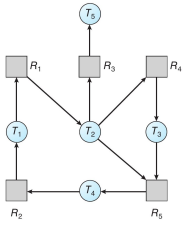
\includegraphics[width = .35\textwidth]{../res/imgs/deadlocks/unsafe.png}
    \hspace{5em}
    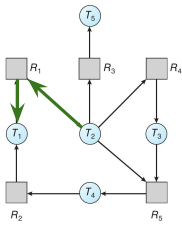
\includegraphics[width = .35\textwidth]{../res/imgs/deadlocks/safe.png}
    \caption{Differenza tra situazione unsafe e safe.}
    \label{fig:safe_unsafe}
\end{figure}
Nel secondo grafo invece si è in una situazione safe in quanto esiste una sequenza dove tutti i processi possono essere eseguiti senza entrare in una condizione di deadlock: $T_1 \to T_4 \to T_3 \to T_5 \to T_2$ infatti è una sequenza che permette il completamento dell'esecuzione dei threads. Anche in questo caso possiamo riassumere tutto in un piccolo \textit{decision tree}:
\begin{figure}[h]
    \centering

    \begin{tikzpicture}
  [
    grow                    = down,
    sibling distance        = 10em,
    level distance          = 6em,
    edge from parent/.style = {draw, -latex},
    every node/.style       = {font=\footnotesize},
    sloped
  ]
  \node [root] {Sei in un safe state?}
    child { node [env] {È possibile\\che ci siano,\\non è sicuro.}
        edge from parent node [above] {No}}
    child { node [env] {Non ci sono\\deadlock.}
      edge from parent node [above] {Si} };
\end{tikzpicture}
\end{figure}

\noindent Ricordiamo infine che gli algoritmi che vedremo in questo paragrafo al fine di prevenire i deadlock \textbf{evitano} di entrare in \textbf{unsafe state}, rimanendo quindi in safe state.
% 
\subsection{Algoritmo sul grafo risorsa-allocazione}
Iniziamo con un algoritmo che funziona solo nel caso di \textbf{risorse singole}, ovvero nel caso in cui si ha solo un pallino ($\bullet$) nel grafo, e quindi ogni tipi di risorsa ha una sola istanza. Introduciamo ora la nozione di \textbf{claim edge} ovvero un arco tratteggiato che indica che il processo $T_i$ può richiedere la risorsa $R_j$. Questi archi diventano \textbf{request edge} nel momento in cui si effettua la richiesta e poi si trasformano a loro volta in \textbf{assignements edge} nel momento in cui stanno utilizzando la risorsa. Osservando il grafo in figura \ref{fig:claim_edge} notiamo che $T_1 \to R_2$ è un claim edge, $T_2 \to R_1$ è un request edge e $R_1 \to T_1$ è un assigmenent edge. 
\begin{figure}[h]
    \centering
    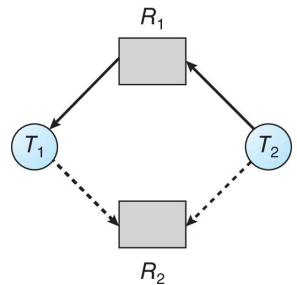
\includegraphics[width = .4\textwidth]{../res/imgs/deadlocks/claim_edge.png}
    \caption{Un grafo composto da tutti e tre i tipi di archi.}
    \label{fig:claim_edge}
\end{figure}

Nella situazione presentata in figura \ref{fig:claim_edge}, si rischia di essere in una situazione \textit{unsafe}. Questo perché se $R_2$ è assegnata al thread $T_2$ nel caso in cui il thread $T_1$ effettui la richiesta per $R_2$ si è in una situazione di deadlock. Possiamo infatti osservare che si ha la presenza di un ciclo e che tutte le risorse abbiano un'istanza, facendo riferimento allo schema in figura \ref{fig:deadlock_decision_tree}, si ha che si è sicuramente in una situazione di deadlock. Ponendo infatti che $R_2$ venga assegnata a $T_2$, nel momento in cui $T_1$ effettui una richiesta, l'algoritmo la nega, in modo tale da non essere in una situazione di deadlock.
\begin{figure}[h]
    \centering
    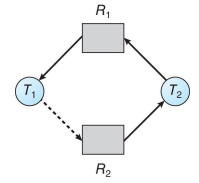
\includegraphics[width = .4\textwidth]{../res/imgs/deadlocks/request_denied.png}
    \caption{L'algoritmo nega la richiesta di $T_1$ per $R_2$}
    \label{fig:request_denied}
\end{figure}
% 
\subsection{Algoritmo del banchiere}
Passiamo ora ad una situazione più reale, quella in cui esistono più risorse con più istanze ciascuna. L'algoritmo a cui si fa affidamento è detto \textit{Banker's algorithm}, ovvero l'algoritmo del banchiere.

Innanzitutto, definiamo con $n$ il numero di processi ed $m$ il numero di tipi di risorse; definiamo poi tre matrici e un'array, strutture sul quale l'algoritmo si appoggia:
\vspace{-15pt}
\begin{itemize}
\setlength{\itemsep}{-.15 em}
    \item L'array \textbf{avaiable} (disponibili) che indica quante istanze di risorse sono disponibili per ogni tipo. Per esempio, la risorsa $j$ ha a disposizione 3 istanze, e questo $\forall j\in[0,m]$.
    \item La prima matrice, \textbf{max} che indica il massimo numero di istanze della risorsa $j$esima che il processo $i$esimo ha al più bisogno ($\forall i\in[0,n]$).
    \item La seconda matrice \textbf{allocated} (allocato), che indica quante istanze della risorsa $j$esima il processo $i$esimo ha già allocato.
    \item La terza matrice, \textbf{need} (bisogno), che non è altro che la differenza tra $max$ e $allocated$; questa matrice indica di quante altre istanze della risorsa $j$esima il processo $i$esimo potrebbe, al più, aver bisogno.
\end{itemize}

Per capire l'algoritmo al meglio si può tranquillamente trascurare lo pseudo-codice e partire subito con un \textbf{esempio}. Abbiamo $n = 5$ thread, da $T_0$ a $T_4$, e 3 tipi di risorse: A, con 10 istanze, B, con 5 e C, che ha a disposizione 7 istanze. Al tempo iniziale $t_0$, la situazione è la seguente:
\begin{table}[!h]
    \centering
    \begin{tabular}{c}
         \underline{\textit{Threads}} \\\\ $T_0$ \\ $T_1$ \\ $T_2$ \\ $T_3$ \\ $T_4$
    \end{tabular}
    \begin{tabular}{c c c}
         \multicolumn{3}{c}{\underline{\textit{Allocated}}} \\
         \textbf{A} & \textbf{B} & \textbf{C} \\
         0 & 1 & 0 \\
         2 & 0 & 0 \\
         3 & 0 & 2 \\
         2 & 1 & 1 \\
         0 & 0 & 1
    \end{tabular}
    \hspace{5px}
    \begin{tabular}{c c c}
         \multicolumn{3}{c}{\underline{\textit{Max}}} \\
         \textbf{A} & \textbf{B} & \textbf{C} \\
         7 & 5 & 3 \\
         3 & 2 & 2 \\
         9 & 0 & 2 \\
         2 & 2 & 2 \\
         4 & 3 & 3 \\
    \end{tabular}    
\end{table}

\noindent Un esempio di lettura della tabella è il seguente: $T_0$ detiene un'istanza di tipo B e zero istanze di tipo A e C. Può richiedere un massimo di 7 istanze di tipo A, 5 istanze di tipo B e 3 istanze di tipo C.

Con questi dati possiamo ora calcolare le due strutture che ci mancano: \textit{Avaiable} e \textit{Need}, che rispettivamente indicano le risorse che sono disponibili (per ogni tipo) e il numero di risorse che un determinato thread può richiedere. Osserviamo che per calcolare il vettore di risorse disponibili è necessario sottrarre alle istanze iniziali la somma delle risorse occupate dai threads. Per esempio, nel caso delle istanze disponibili della risorsa A abbiamo che sono $10 - (2 + 3 + 2) = 3$, occupate rispettivamente da: $T_1$, $T_2$ e $T_3$. per calcolare invece la matrice \textit{Need}, per ogni cella della matrice si sottrarre il valore di \textit{Max} al valore di $Allocated$ nella cella $[i,j]$.
\begin{table}[h!]
    \centering
        \begin{tabular}{c c c}
         \multicolumn{3}{c}{\underline{\textit{Avaiable}}} \\
         \textbf{A} & \textbf{B} & \textbf{C} \\
         3 & 3 & 2
    \end{tabular}
    \hspace{5pt}    
    \begin{tabular}{c c c}
         \multicolumn{3}{c}{\underline{\textit{Need}}} \\
         \textbf{A} & \textbf{B} & \textbf{C} \\
         7 & 4 & 3 \\
         1 & 2 & 2 \\
         6 & 0 & 0 \\
         0 & 1 & 1 \\
         4 & 3 & 1 \\
    \end{tabular}
\end{table}

Abbiamo ora tutte le risorse necessarie per iniziare a eseguire l'algoritmo. Iniziamo scorrendo la matrice \textit{Need} e comparandola con il vettore \textit{Avaiable}. Partiamo dal thread $T_0$: con le risorse disponibili $[3,3,2]$, il thread ha la possibilità di terminare? No, perché per terminare necessita, al più, di 7 istanze di A, 4 istanze di B e 3 istanze di C. Passiamo ora al secondo thread: $T_1$ può terminare con le risorse disponibili? Si, perché tutte le risorse di cui ha bisogno sono $\leq$ rispetto alle risorse disponibili. A questo punto allora si spostano le risorse necessarie a $T_1$ per terminare, ovvero $[1,2,2]$:

\begin{table}[h]
    \centering
    \begin{tabular}{c}
         \underline{\textit{Threads}} \\\\ $T_0$ \\ $T_1$ \\ $T_2$ \\ $T_3$ \\ $T_4$
    \end{tabular}
    \begin{tabular}{c c c}
         \multicolumn{3}{c}{\underline{\textit{Allocated}}} \\
         \textbf{A} & \textbf{B} & \textbf{C} \\
         0 & 1 & 0 \\
         \textbf{3} & \textbf{2} & \textbf{2} \\
         3 & 0 & 2 \\
         2 & 1 & 1 \\
         0 & 0 & 1
    \end{tabular}
    \hspace{5px}
    \begin{tabular}{c c c}
         \multicolumn{3}{c}{\underline{\textit{Max}}} \\
         \textbf{A} & \textbf{B} & \textbf{C} \\
         7 & 5 & 3 \\
         3 & 2 & 2 \\
         9 & 0 & 2 \\
         2 & 2 & 2 \\
         4 & 3 & 3 \\
    \end{tabular}    
    \hspace{5pt}    
    \begin{tabular}{c c c}
         \multicolumn{3}{c}{\underline{\textit{Need}}} \\
         \textbf{A} & \textbf{B} & \textbf{C} \\
         7 & 4 & 3 \\
         0 & 0 & 0 \\
         6 & 0 & 0 \\
         0 & 1 & 1 \\
         4 & 3 & 1 \\
    \end{tabular}
    \hspace{5pt}
    \begin{tabular}{c c c}
         \multicolumn{3}{c}{\underline{\textit{Avaiable}}} \\
         \textbf{A} & \textbf{B} & \textbf{C} \\
         \textbf{2} & \textbf{1} & \textbf{0}
    \end{tabular}
\end{table}
\pagebreak Una volta terminato il thread $T_1$, le risorse vengono rilasciate e il vettore \textit{Avaiable} va aggiornato, sommando alle risorse disponibili le risorse che sono appena state rilasciate da $T_1$.
\begin{table}[h!]
    \centering
    \begin{tabular}{c c c}
         \multicolumn{3}{c}{\underline{\textit{Avaiable}}} \\
         \textbf{A} & \textbf{B} & \textbf{C} \\
         5 & 3 & 2
    \end{tabular}
\end{table}

A questo punto ci sono abbastanza risorse per terminare un altro processo come, per esempio $T_3$ oppure $T_4$. Così facendo, mano che i thread vengono eseguiti e terminati vengono rilasciate abbastanza risorse per completare quelli più onerosi. Una sequenza esempio dell'ordine con il quale i thread sono completati può essere: \{$T_1,T_3,T_4,T_2,T_0$\}. 

Può succedere che durante l'esecuzione dei thread possono arrivare altre richieste che devono essere accettate o meno. Per esempio se prima dell'esecuzione $T_4$ avesse fatto una richiesta $[3,3,0]$, la richiesta sarebbe stata rifiutata dato che le risorse disponibili erano minori rispetto alla richiesta.
% 
\section{Detection}
L'ultimo approccio che andiamo a discutere è il rilevamento del deadlock: si va alla ricerca di tale e, una volta trovato, si passa al salvataggio, alla \textbf{recovery}. Anche in questo caso, come per l'approccio di \textit{avoidance} (paragrafo \ref{avoidance}) sono presenti due algoritmi, uno studiato per avere solo un'istanza per risorsa e il secondo che copre anche il caso in cui ci siano più istanze per risorse.



\subsection{Istanza singola}
In questo primo caso si fa riferimento ad un secondo grafo particolare chiamato \textbf{wait-for graph}. È una modifica del \textit{resource-allocation graph} dove si evidenzia il fatto che un thread sta aspettando il termine dell'esecuzione di un altro thread: non sono infatti presenti vertici che rappresentano risorse a ci sono solo nodi che indicano i thread.
\begin{figure}[h]
    \centering
    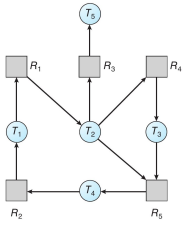
\includegraphics[width = .25\textwidth]{../res/imgs/deadlocks/unsafe.png}
    \hspace{10pt}
    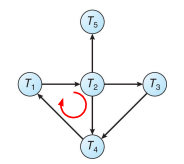
\includegraphics[width = .35\textwidth]{../res/imgs/deadlocks/wait-for_graph.png}
    \caption{Un grafo \textit{resource-allocation} e il suo rispettivo \textit{wait-for graph}}
    \label{fig:wait-for}
\end{figure}
In figura \ref{fig:wait-for} si osserva la traduzione di un grafo risorsa allocazioni in gra grafo \textit{wait-for}. Si nota che nel secondo grafo si accetua ancora di più la presenza di cicli e, dato che is tratta di risorse con istanza singola, la presenza di un ciclio ha l'immediata conseguenza di generare una situazione di deadlock.

L'algoritmo di cui stiamo parlando infatti, per rilevare un deadlock, si limita a creare un \textit{wait-for graph} e controllare la presenza di cicli\footnote{Da studente che ha seguito il corso "Dati e Algoritmi" penso che si utilizzino algoritmi basati su BFS oppure DFS.}. Una volta trovato il ciclo si è sicuri di aver trovato il deadlock e si passa alla \textit{deadlock recovery} (vedi paragrafo \ref{recovery}). Possiamo quindi notare che nella figura \ref{fig:wait-for} si è in una condizione di deadlock dato che il thread $T_1$ sta attendendo il termine di $T_2$ che è in attesa di $T_4$ che a sua volta sta aspettando $T_1$. Una situazione analoga è presente anche con i thread $T_1,T_2,T_3,T_4$.
% 
\subsection{Istanze multiple}
Nel caso invece delle istanze multiple, anche in questo algoritmo si fa affidamento a diverse strutture dati, proprio come nell'algoritmo del banchiere. Avremo quindi a che vedere con $n$ processi che hanno a che fare con $m$ tipi di risorse che interagiranno con due matrici e un vettore.
\vspace{-5px}
\begin{itemize}
\setlength{\itemsep}{-.15 em}
    \item Il vettore \textit{Avaiable}, proprio come nell'algoritmo del banchiere, tiene traccia di quante istanze sono libere per ogni tipo di risorsa.
    \item La prima matrice \textit{Allocated} memorizza il numero di risorse che ogni processo detiene.
    \item La seconda matrice, \textbf{Request}, indica quante risorse il thread sta richiedendo al fine di terminare.
\end{itemize}

Come nel caso dell'algoritmo del banchiere, non ci soffermiamo sullo pseudo-codice ma partiamo subito con un esempio. Poniamo di avere cinque threads, da $T_0$ a $T_4$ e di avere anche in questo caso tre tipi di risorse: A, con 7 istanze, B con 2 istanze e C con 6 istanze. Al tempo iniziale $t_0$ ci troviamo nella seguente situazione:
\begin{table}[h]
    \centering
    \begin{tabular}{c}
         \underline{\textit{Threads}} \\\\ $T_0$ \\ $T_1$ \\ $T_2$ \\ $T_3$ \\ $T_4$
    \end{tabular}
    \begin{tabular}{c c c}
         \multicolumn{3}{c}{\underline{\textit{Allocated}}} \\
         \textbf{A} & \textbf{B} & \textbf{C} \\
         0 & 1 & 0 \\
         2 & 0 & 0 \\
         3 & 0 & 3 \\
         2 & 1 & 1 \\
         0 & 0 & 2 \\
    \end{tabular}
    \hspace{5px}
    \begin{tabular}{c c c}
         \multicolumn{3}{c}{\underline{\textit{Request}}} \\
         \textbf{A} & \textbf{B} & \textbf{C} \\
         0 & 0 & 0 \\
         2 & 0 & 2 \\
         0 & 0 & 0 \\
         1 & 0 & 0 \\
         0 & 0 & 2 \\
    \end{tabular} 
    \hspace{5pt}
    \begin{tabular}{c c c}
         \multicolumn{3}{c}{\underline{\textit{Avaiable}}} \\
         \textbf{A} & \textbf{B} & \textbf{C} \\
         0 & 0 & 0 
    \end{tabular}
\end{table}

\noindent Dalla tabella \textit{Request} possiamo notare che sia $T_0$ che $T_2$ possono completare senza attendere altri processi dato che non richiedono nulla. Una volta terminati $T_0$ e $T_2$ tutti gli altri thread possono man mano terminare. Non siamo quindi in una situazione di deadlock.

Mettiamoci però nel caso in cui $T_2$ debba richiedere una risorsa di tipo C.
\begin{table}[h]
    \centering
    \begin{tabular}{c}
         \underline{\textit{Threads}} \\\\ $T_0$ \\ $T_1$ \\ $T_2$ \\ $T_3$ \\ $T_4$
    \end{tabular}
    \begin{tabular}{c c c}
         \multicolumn{3}{c}{\underline{\textit{Allocated}}} \\
         \textbf{A} & \textbf{B} & \textbf{C} \\
         0 & 1 & 0 \\
         2 & 0 & 0 \\
         3 & 0 & 3 \\
         2 & 1 & 1 \\
         0 & 0 & 2 \\
    \end{tabular}
    \hspace{5px}
    \begin{tabular}{c c c}
         \multicolumn{3}{c}{\underline{\textit{Request}}} \\
         \textbf{A} & \textbf{B} & \textbf{C} \\
         0 & 0 & 0 \\
         2 & 0 & 2 \\
         0 & 0 & \textbf{1} \\
         1 & 0 & 0 \\
         0 & 0 & 2 \\
    \end{tabular} 
    \hspace{5pt}
    \begin{tabular}{c c c}
         \multicolumn{3}{c}{\underline{\textit{Avaiable}}} \\
         \textbf{A} & \textbf{B} & \textbf{C} \\
         0 & 0 & 0 
    \end{tabular}
\end{table}
In questo caso le risorse che vengono rilasciate al termine di $T_0$ non sono necessarie per terminare gli altri thread e ci troveremo quindi in una situazione di deadlock.
% 
\subsection{Deadlock recovery}\label{recovery}
Come dobbiamo comportarci nel momenti in cui rileviamo un deadlock? La soluzione più brutale è quella di terminare tutti i processi che si trovano all'interno del deadlock (come fare un \texttt{CTRL + C} ad ogni processo). Esiste però un altro modo un po' più elegante che fa comunque affidamento alla \textbf{terminazione dei processi}: si cerca infatti di terminare ad uno ad uno tutti i thread che compongono il ciclo. L'ordine di terminazione può essere scelto in base alla priorità, in base alle risorse che il thread ha utilizzato o altro.

Una seconda strada invece si basa sul \textbf{resource preemption}, ovvero sul rubare delle risorse che sono detenute da un altro processo o thread. In questo caso si sceglie una vittima a cui rubare le risorse e si cerca di far terminare un thread. Si ricorda che anch ein questo caso si può arrivare ad una situazione di \textit{starvation} se lo stesso thread è sempre preso come vittima.



\newpage\part{Gestione della Memoria}

\pagebreak
\section{Memoria principale}\label{main memory}
Fino ad ora abbiamo discusso di come un sistema operativo gestisce lo scheduling (\ref{CPU scheduling}), la sincronizzazione (\ref{sincronizzazione}) e i deadlock (\ref{deadlocks}) sorvolando sempre sulla locazione effettiva su cui questi processi vengono mantenuti, ovvero la memoria. Osserviamo sin dall'inizio che con memoria intendiamo la memoria RAM del calcolatore, le memorie secondarie molto capienti sono i dischi e le memorie di massa, che verranno discusse approfonditamente nel capitolo \ref{mass memory}. In particolare in questo capitolo ci occuperemo di dare un'introduzione ai concetti generali, passando poi a discutere il metodo più semplice per risolvere l'utilizzo della memoria, ovvero l'allocazione continua per poi discutere un tecnica più avanzata che tutt'ora si trova nei sistemi operativi moderni, ovvero il \textit{paging}. Scopriremo che saranno necessarie delle strutture ausiliarie, come la tabella delle pagine, e ne studieremo i diversi metodi di implementazione. Infine ci dedicheremo al concetto di \textit{swapping} e a modelli di allocazioni alternativi alla paginazione.

\subsection{Introduzione}
Come sappiamo, il programma, una volta che viene eseguito, deve essere caricato dal disco in memoria. Solo una volta che è stato caricato in memoria può essere eseguito; questo perché la CPU non ha accesso diretto alla memoria di massa. Sappiamo inoltre che l'accesso della CPU è effettuato seguendo 3 tipi di memorie (figura \ref{fig:memory_hierarchy}):
\vspace{-5px}
\begin{itemize}
\setlength{\itemsep}{-.15 em}
    \item Registri, che hanno un accesso rapidissimo;
    \item RAM, che ha una velocità sicuramente ridotta rispetto ai registri;
    \item \textbf{Cache}, che è una piccola memoria che fa da intermediario tra i registri e la RAM ed ha un tempo di accesso molto più veloce della memoria.
\end{itemize}
\begin{figure}[h]
    \centering
    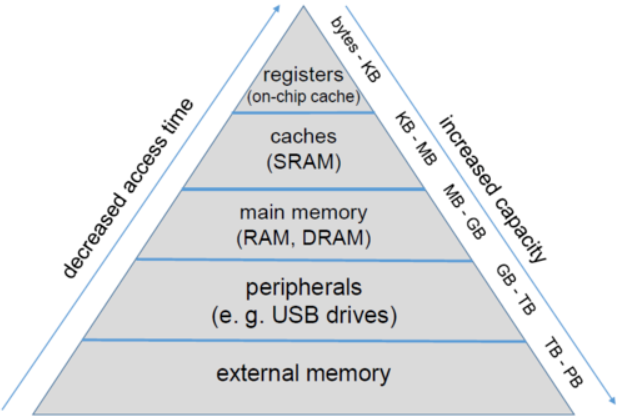
\includegraphics[width = .5\textwidth]{../res/imgs/main memory/memory_hierarchy.png}
    \caption{La gerarchie delle memorie nel calcolatore.}
    \label{fig:memory_hierarchy}
\end{figure}

% 
\subsubsection{Protezione}
In generale, se vogliamo avere molti processi che vengono caricati contemporaneamente nell'area della memoria e che vengono eseguiti in modo concorrente, è importante che ci sia una protezione dei processi fornita dal sistema operativo al fine di garantire che ogni processo abbia il suo spazio di memoria senza che vada a collidere con un altro processo. La soluzione più banale, rappresentata in figura \ref{fig:process_protection}, è quella di utilizzare due registri che tengono traccia di due valore: l'indirizzo \textbf{base}, ovvero l'indirizzo in memoria iniziale da cui il processo parte, e il valore \textbf{limite} (\textit{offset}) che indica la massima espansione del processo in memoria. In altre parole, il processo in memoria non può superare l'indirizzo "base + limite" (più avanti in questo capitolo vedremo soluzione più complesse e raffinate).
\begin{figure}[h]
    \centering
    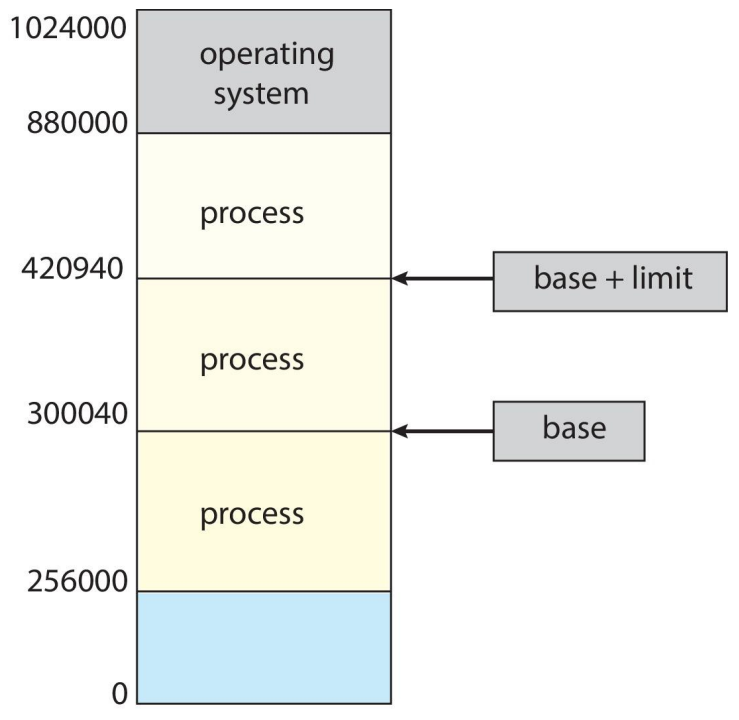
\includegraphics[width = .35\textwidth]{../res/imgs/main memory/process_protection.png}
    \caption{Limite inferiore e limite superiore dello spazio del processo in memoria.}
    \label{fig:process_protection}
\end{figure}
In questo caso l'unica preoccupazione del sistema operativo è controllare, ogni volta che un indirizzo viene generato dalla CPU durante l'esecuzione del programma, se questo indirizzo è compreso tra la base e l'offset fornito dai due registri. Nel caso in cui l'indirizzo è compreso allora la locazione di memoria può essere acceduta. Osserviamo che la figura \ref{fig:can_access} rappresenta un piccolo schema dove viene illustrata questa verifica da parte del sistema operativo.
\begin{figure}[h]
    \centering
    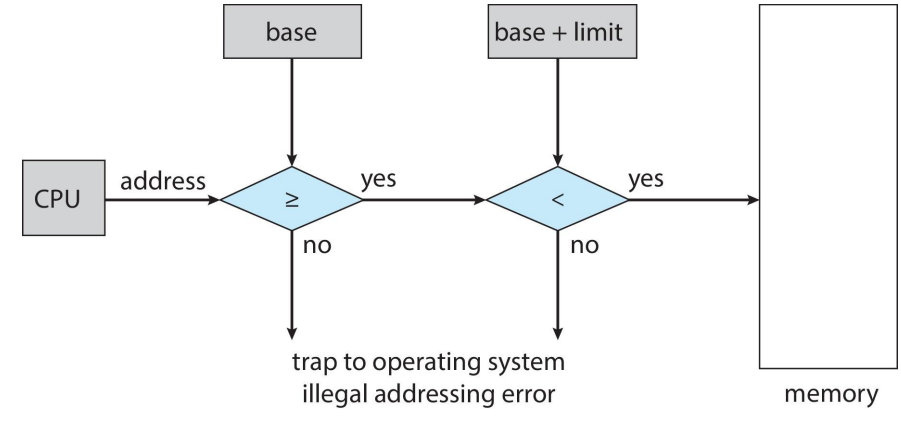
\includegraphics[width = .6\textwidth]{../res/imgs/main memory/can_access.png}
    \caption{Procedura di controllo di un indirizzo mediante il SO.}
    \label{fig:can_access}
\end{figure}

% 
\subsubsection{Binding}
Quando creiamo un processo, di default parte dall'allocazione 0000. Naturalmente non è possibile far partire tutti i processi dalla stessa allocazione altrimenti si genererebbero conflitti che causerebbero problemi non indifferenti. Inoltre ogni processo che viene eseguito, anche se il suo indirizzo in memoria è diverso 0000, viene eseguito come se la sua prima cella disponibile fosse la 0000. Come è possibile? Il procedimento è chiamato \textbf{binding} e mappa due tipi di indirizzi: gli indirizzi \textbf{assoluti}, che sono gli effettivi indirizzi nella memoria, e gli indirizzi \textbf{rilocabili} che sono gli indirizzi relativi al programma in esecuzione. Per chiarire le idee, facciamo un esempio: poniamo di avere un processo che parte dall'indirizzo in memoria \texttt{31400} (indirizzo assoluto) e che stia eseguendo una linea di codice che secondo il processo è all'indirizzo \texttt{15}. In realtà il programma non sta eseguendo l'indirizzo \texttt{15} ma sta eseguendo l'indirizzo assoluto \texttt{31415}, che è la somma tra l'indirizzo fisico di inizio e l'indirizzo logico (31400 + 15). Questa somma, è infatti detta binding e permette di collegare gli indirizzi logici del processo agli indirizzi fisici della memoria. 

\begin{wrapfigure}{o}{.30\textwidth}
  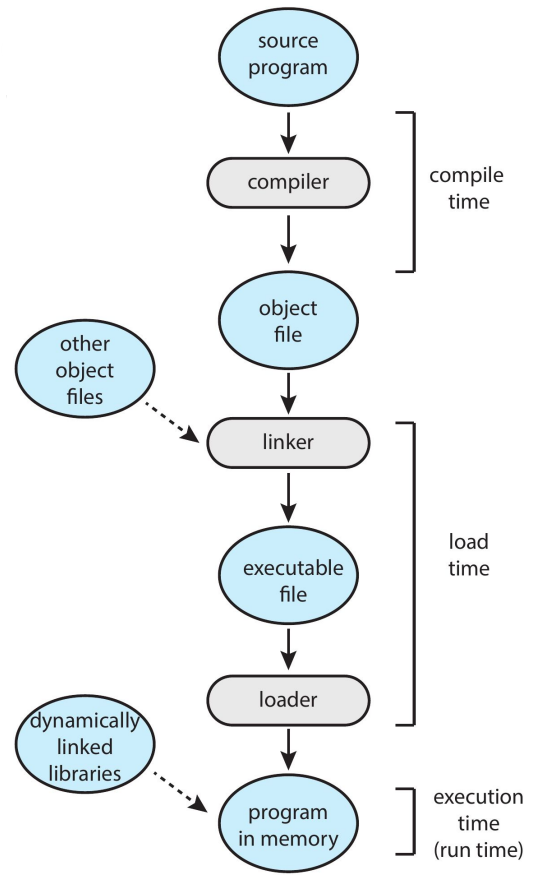
\includegraphics[width = \linewidth]{../res/imgs/main memory/binding_time.png}
  \caption{I tre tempi di binding.}
  \label{fig:binding_time}
\end{wrapfigure}
Il binding però può avvenire in diversi momenti, come è possibile anche osservare dalla figura \ref{fig:binding_time}. Possiamo distinguere principalmente 3 momenti:
\vspace{-5px}
\begin{enumerate}
\setlength{\itemsep}{-.15 em}
    \item Tempo di \textbf{compilazione}: in questo caso, il compilatore, compilando il codice automaticamente converte gli indirizzi rilocabili in indirizzi assoluti.
    \item Tempo di \textbf{caricamento}: nel momento di \textit{linking} del programma e quindi si ha un eseguibile che ha ancora gli indirizzi temporanei ma che poi, una volta caricato, verranno sostituiti con gli indirizzi assoluti.
    \item Tempo di \textbf{esecuzione}: è infine possibile trasformare gli indirizzi rilocabili in indirizzi assoluti durante l'esecuzione del programma. Questo è il metodo tipicamente utilizzato dai sistemi operativi moderni, attraverso tecniche che approfondiremo in questo capitolo.
\end{enumerate}

È quindi fare un'importante distinzione tra due tipi di indirizzi. Lo spazio di indirizzi che è visto dal programma (e quindi è indipendente dalla macchina in cui risiede) è chiamato spazio degli indirizzi \textbf{logici} (o \textbf{virtuali}, come vedremo nel capitolo \ref{virtual memory}). D'altro canto, lo spazio degli indirizzi in memoria, ovvero gli indirizzi assoluti, è chiamato spazio degli indirizzi \textbf{fisici}. 

% 
\subsubsection{Memory-Management Unit (MMU)}
Parte dei meccanismo utilizzati per gestire la memoria e il binding non sono lasciati solamente al sistema operativo ma sono un ibrido tra hardware e software. Questo hardware è detto \textit{Memory-Management Unit} (\textbf{MMU}) ed aiuta a mappare gli indirizzi logici in indirizzi fisici. Questo modulo era originariamente un chip a parte, tra la CPU e la memoria, con l'avanzare del tempo l'MMU è una parte integrata nella CPU stessa.

Una delle funzionalità dell'MMU è quella di fornire il controllo sull'indirizzo del processo nella memoria. È la stessa funzionalità che implementava il sistema operativo (vedi figura \ref{fig:can_access}) solo che in questo caso il controllo è effettuato autonomamente dell'MMU attraverso un particolare registro chiamato \textbf{relocation register}. Il processo è rappresentato nell'illustrazione \ref{fig:can_access_MMU}.

\begin{figure}[h]
    \centering
    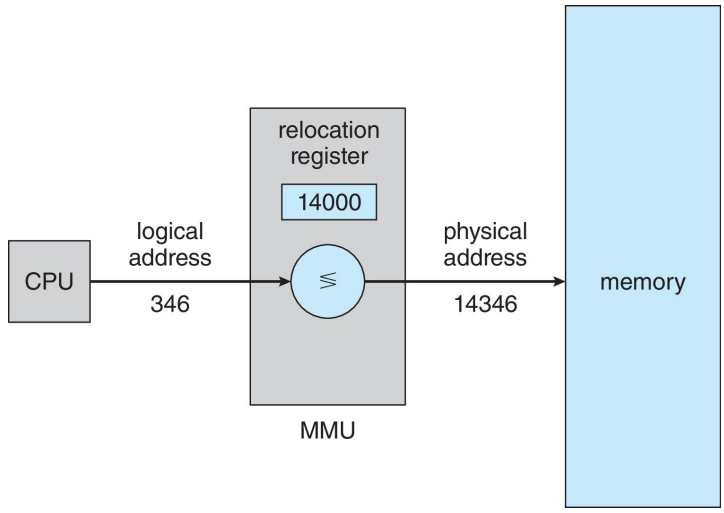
\includegraphics[width = .55\textwidth]{../res/imgs/main memory/can_access_MMU.png}
    \caption{Procedura di controllo di un indirizzo mediante la MMU.}
    \label{fig:can_access_MMU}
\end{figure}

% 
\subsubsection{Caricamento e collegamento dinamico}\label{dynamic loading and linking}
Uno dei concetti fondamentali nell'uso della memoria è il \textbf{dynamic loading}. Ciò significa che dal punto di vista del programma non è possibile mantenere tutte le funzioni necessarie del programma sempre in memoria, ma mantenere solo un sottoinsieme che sono al momento necessarie. Nel momento in cui una nuova routine è necessaria la si va a caricare dalla memoria.

Un secondo approccio è quello del \textit{linking}. In particolare il collegamento può essere fatto in due modi: statico e dinamico. Lo \textbf{static linking} avviene quando colleghiamo le librerie di sistema al programma e una volta compilato il programma le librerie sono immediatamente integrate nel file eseguibile. A questo si contrappone il \textbf{dynamic linking} dove il codice delle librerie non viene caricato nel file eseguibile ma le librerie sono collegate solo durante l'esecuzione del programma. Sono infatti presenti delle \textbf{shared libraries}, come le \texttt{dll} di Windows, che vengono caricate in memoria e condivise a tutti i processi che le necessita e, un volta che nessun processo le utilizza più, queste vengono rimosse dalla memoria. Questo è molto più conveniente rispetto al collegamento statico dove in memoria ci possono essere potenzialmente diversi programmi che hanno una copia della libreria nel codice. Questo significa che la stessa libreria occupa molto più spazio in memoria perché è copiata da diversi processi. Se invece ci fosse stata una librerie dinamica, tutti i processi avrebbero usufruito il codice della stessa in modo tale da risparmiare dello spazio prezioso in memoria.

% 
\subsection{Primi modelli di allocazione}
Passiamo ora a vedere la storia e i concetti della paginazione della memoria per poi arrivare a discutere dei metodi moderni e tuttora utilizzati.

% 
\subsubsection{Allocazione contigua}
La prima soluzione che è stata pensata è l'allocazione contigua (figura \ref{fig:memory_contiguos_allocation}) in memoria: 
\begin{figure}[h]
    \centering
    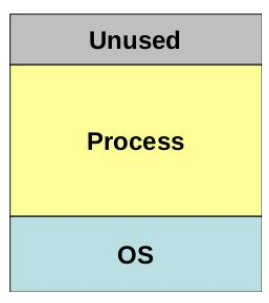
\includegraphics[width = .15\textwidth]{../res/imgs/main memory/contiguos_allocation.png}
    \caption{Allocazione contigua dei processi in memoria.}
    \label{fig:memory_contiguos_allocation}
\end{figure}
ciò significa avere una parte dedicata al sistema operativa (kernell) e poi, in modo contiguo, inizia il codice per i processi.

Il modo più semplice per poter implementare questo meccanismo è attraverso il \textit{limit register} e il \textit{reloction register} che abbiamo visto poco fa. Questo infatti permette di proteggere i processi tra di loro, evitando quindi che si sovrappongano in memoria. Osservando infatti l'illustrazione \ref{fig:relocation_register_allocation} possiamo notare che dalla CPU viene preso l'indirizzo logico (ovvero l'indirizzo relativo per il processo), viene controllato se "sfora" il limite massimo in memoria; una volta che è stato appurato che l'\textit{upper bound} non è stato superato, il relocation register procede con il \textit{binding}.
\begin{figure}[h]
    \centering
    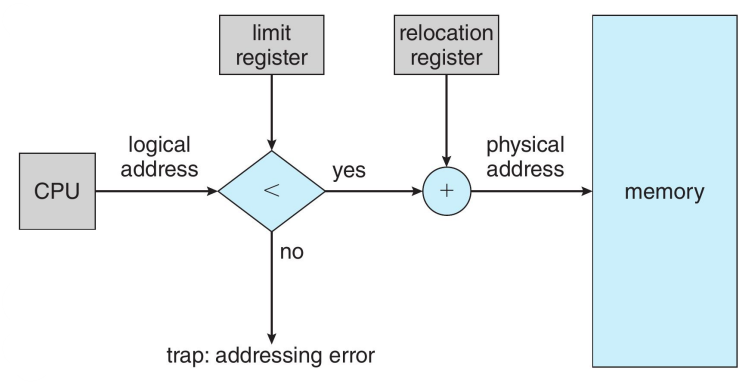
\includegraphics[width = .5\textwidth]{../res/imgs/main memory/relocation_register_allocation.png}
    \caption{I registri utilizzati per il binding tra logico e fisico.}
    \label{fig:relocation_register_allocation}
\end{figure}

% 
\subsubsection{Allocazione a partizione fissa}\label{partizione_fissa}
Un a soluzione un po' più raffinata, è l'allocazione a partizione fisse. Questo tipo di allocazione consiste nel dividere la memoria in un insieme di partizioni di dimensione non variabile e andare ad allocare i processi, non in modo contiguo, ma in una partizione la cui dimensione è adeguata e consona alla dimensione del processo. 
\begin{figure}[h]
    \centering
    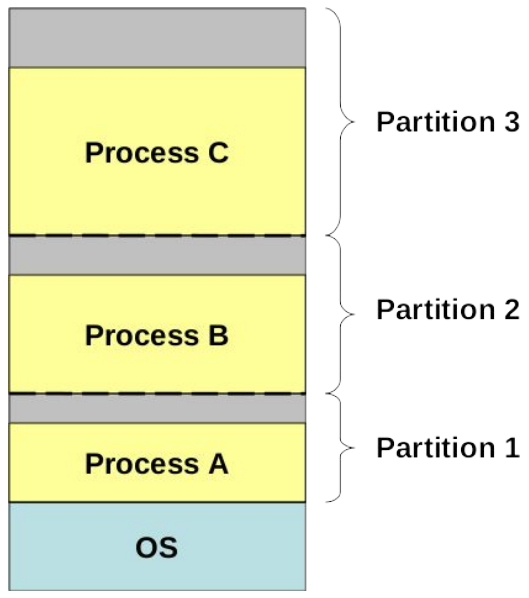
\includegraphics[width = .28\textwidth]{../res/imgs/main memory/fixed_partition.png}
    \caption{La memoria divisa in partizioni fisse per i processi.}
    \label{fig:fixed_partition}
\end{figure}
Osservando la figura \ref{fig:fixed_partition} notiamo che, innanzitutto le partizioni possono essere di dimensione diversa (l'importante è che non cambi nel tempo) al fine di gestire processi si dimensione diversa. Notiamo già i possibili problemi di questo tipo di modello, primo tra tutti è lo spazio in memoria inutilizzato grigio alla fine di ogni partizione (vedi il paragrafo \ref{frammentazione}: frammentazione interna). L'idea però della partizioni fisse è un concetto che, come vedremo verrà ripreso nella paginazione (paragrafo \ref{paginazione}), presente nei sistemi operativi moderni.

% 
\subsubsection{Allocazione a partizione variabile}\label{partizione_variaibile}
In alternativa alla partizione fissa, possiamo avere un tipo di allocazione in cui la dimensione della partizione varia a seconda del processo che fa richiesta. Osservando l'illustrazione \ref{fig:variable_partition} notiamo che il processo 8, una volta che è terminato lascia un buco ad un secondo processo, il 9 che però occupa meno spazio, di conseguenza la dimensione della partizione è variata.
\begin{figure}[h]
    \centering
    \includegraphics[width = .55\textwidth]{../res/imgs/main memory/variable_partition.png}
    \caption{Rappresentazione di una partizione variabile in memoria.}
    \label{fig:variable_partition}
\end{figure}
Anche in questo caso, come nella partizione fissa, si può incombere in una frammentazione interna (paragrafo \ref{frammentazione}) dato che una volta che il processo 9 ha occupato lo spazio rilasciato dal processo 8, è rimasto comunque un \textbf{buco} in memoria, che non sempre può essere occupato da un altro processo in quanto, magari, non è presente abbastanza spazio contiguo.

% 
\subsubsection*{Scelta della cella da allocare}
Poniamo di essere in una situazione in cui abbiamo alcuni processi sparsi in memoria ed è necessario inserire un nuovo processo, come in figura \ref{fig:allocation_choice}. Quale posto scegliamo?
\begin{figure}[h]
    \centering
    \includegraphics[width = .4\textwidth]{../res/imgs/main memory/allocation_choice.png}
    \caption{In quale allocazione di memoria verrà inserito il nuovo processo?}
    \label{fig:allocation_choice}
\end{figure}

\noindent La scelta può essere effettuata secondo 3 criteri diversi:
\vspace{-5px}
\begin{itemize}
\setlength{\itemsep}{-.15 em}
    \item \textit{First-fit}: il primo posto disponibile viene occupato dal nuovo processo. Per esempio, se abbiamo la memoria ad allocazione variabile e all'interno di essa abbiamo un processo B e un processo C, si va a scorrere la memoria e si inserisce il nuovo processo nel primo \textit{hole} disponibile;
    \item \textit{Best-fit}: in questo caso si cerca di allocare il nuovo processo nella zona il più si avvicina alla dimensione del processo. Di conseguenza, al fine di allocare il processo in memoria è prima necessario scorrerla tutta con una ricerca \textbf{lineare};
    \item \textit{Worst-fit}: infine, con questa tecnica, si sceglie lo spazio con la dimensione peggiore possibile, ovvero la dimensione più grande possibile; ciò significa che il buco lasciato in memoria sarà il più grande possibile. Anche in questo caso è necessario fare una ricerca \textbf{lineare}.
\end{itemize}

% 
\subsubsection{Problema della frammentazione}\label{frammentazione}
Abbiamo ormai constatato che quando si allocano nuovi processi in memoria, questi lasciano in memoria dei buchi che non sempre possono essere riempiti. In particolare, nel caso della partizione fissa (\ref{partizione_fissa}) questo tipo di problema viene chiamato \textbf{frammentazione interna}, questo perché è interna alla partizione in quanto il processo allocato non riesce a riempire pienamente lo spazio della partizione (osservare la figura \ref{fig:fixed_partition}). Questo rappresenta ovviamente un problema perché può essere che in memoria ci sia in totale dello spazio disponibile (ovvero la somma di tutti gli spazi grigi in figura) ma essendo non contiguo non permette un ulteriore inserimento del processo in memoria. 

Alla frammentazione interna si contrappone la \textbf{frammentazione esterna}, che si verifica nel caso dell'allocazione a partizione variabile (\ref{partizione_variaibile}). Facendo appunto riferimento alla figura \ref{fig:variable_partition}, può essere che una volta inserito il processo 9 all'interno della memoria si siano generati due buchi che non sono abbastanza grandi al fine di contenere un altro processo. Si è fatto uno studio dove si è notato che con l'allocazione a partizione variabile e il \textbf{first-fit}, ogni N blocchi in memoria, se ne perdono la metà a causa della frammentazione esterna: di conseguenza all'incirca $1/3$ della memoria è inutilizzato (\textit{50-percent rule}). 

Una soluzione al problema della frammentazione esterna è il \textbf{compacting} (compattazione), illustrata in figura \ref{fig:compacting}. Poniamo che il processo B termini e venga rimosso dalla memoria; si creerebbe un buco sopra e sotto il processo C che non consentirebbe a processi di grandi dimensione di essere inseriti all'interno della memoria.
\begin{figure}[h]
    \centering
    \includegraphics[width = .48\textwidth]{../res/imgs/main memory/compacting1.png}
    \hspace{2em}
    \includegraphics[width = .32\textwidth]{../res/imgs/main memory/compacting2.png}
    \caption{Processo di compacting, una soluzione alla frammentazione esterna.}
    \label{fig:compacting}
\end{figure}
Allora, al posto di lasciare così com'è la memoria, si sceglie di compattare tutti i processi nella parte bassa in memoria al fine di avere un'unica zona di memoria con soli processi (e senza buchi) e una parte in memoria completamente a disposizione dei nuovi processi. Sembrerebbe una soluzione ottimale ma in realtà comporta alcuni diversi problemi. Primo tra tutti è che bisogna capire come \textbf{spostare} dei \textbf{processi} in memoria: fino ad ora venivano inseriti e rimossi ma mai spostati da una zona all'altra. In secondo luogo, se si ripete questo processo per milioni di locazioni in memoria, compattare molti processi diventa un \textbf{problema computazionale} non indifferente, soprattutto se si fa ogni volta che un processo in memoria viene rimosso. È quindi evidente che la soluzione sia tutto fuorché ottimale e che quindi i problemi di frammentazione, con questo tipo di allocazioni, persistono.

% 
\subsection{Paginazione (\textit{paging)}}\label{paginazione}
Ecco quindi che introduciamo questo nuovo tipo di allocazione, molto più moderno ed elegante, ovvero la \textbf{paginazione}. Il concetto alla base di questa tecnica è quello di dividere la memoria in locazioni di dimensione fissa $\overline{n}$, chiamate \textbf{\textit{frames}}, e dividere lo spazio logico dei processi in blocchi della stessa dimensione $\overline{n}$. Generalmente, nei sistemi operativi moderni, $\overline{n}\in [ \texttt{512 Bytes},\texttt{16 MBytes} ]$. In questo modo è quindi possibile dividere i processi in \textbf{pagine} e associare ad ogni pagina di ogni processo in esecuzione un frame in memoria, proprio come illustrato nella figura \ref{fig:paging}.
\begin{figure}[h]
    \centering
    \includegraphics[width = .6\textwidth]{../res/imgs/main memory/paging.png}
    \caption{Il funzionamento ad alto livello della paginazione.}
    \label{fig:paging}
\end{figure}
Questa tecnica risolve subito il problema della frammentazione esterna e dei buchi. Osservando infatti la figura \ref{fig:remove_process_paging}, nel momento in cui il processo B termina l'esecuzione e viene rimosso dalla memoria, dovrebbero rimanere dei buchi tra il processo A e il processo C. Questo buchi però vengono immediatamente colmati dal processo D le quali pagine vengono mappate nei frames che prima erano occupati da B e dal frame seguente al processo C. In questo modo, proprio perché le pagine e i frames sono della stessa dimensione si incastrano perfettamente tra di loro e non lasciano nessun buco.
\begin{figure}[h]
    \centering
    \includegraphics[width = .6\textwidth]{../res/imgs/main memory/remove_process_paging.png}
    \caption{La rimozione di un processo e l'inserimento di un altro con la paginazione.}
    \label{fig:remove_process_paging}
\end{figure}

Se andiamo a dividere lo spazio logico in pagine e la memoria viene divisa in frames, abbiamo bisogno di un supporto che mappa ciascuna pagina del processo ad un frame in memoria. Questo supporto è chiamato \textbf{page table} (discussa approfonditamente nel paragrafo \ref{page_table}) e si occupa appunto della traduzione di indirizzi logici (pagine) in indirizzi fisici (frames). Si osserva che la page table è una struttura associata ad ogni singolo processo. Di conseguenza due processi hanno due page table differenti.

% 
\subsubsection{Frammentazione interna}
Osserviamo infine un'ultima cosa: pur avendo eliminato il problema della frammentazione esterna, la \textbf{frammentazione interna} persiste: molto spesso infatti un processo non avrà esattamente la dimensione di \textit{n} pagine, anzi, avrà generalmente una dimensione che è minore della dimensione occupata da \textit{n} pagine ma comunque più grande di quella occupata da \textit{n-1} pagine. Di conseguenza l'ultima pagina non sarà mai completamente piene ma avrà dello spazio non occupato. Questo spazio non potrà nemmeno essere utilizzato da altri processi dato che come sappiamo la dimensione della pagina è fissa.

Facciamo un esempio per fissare il concetto. Abbiamo un processo di \texttt{10 KBytes} che deve essere allocato in memoria. Poniamo che la dimensione delle pagine (e quindi dei \textit{frames}) è di \texttt{4 KBytes}. Al fine di inserire il processo in memoria sono quindi necessarie 3 pagine, che forniscono uno spazio di \texttt{3 * 4 KBytes = 12 KBytes} che è maggiore rispetto ai \texttt{10 KBytes} del processo: sono quindi sprecati \texttt{12 - 10 = 2 KBytes} che non potranno mai essere occupati da altri processi. Al caso migliore lo spreco è di \texttt{1 Byte} (ovvero la dimensione di 1 cella in memoria), mentre al caso peggiore lo spreco è di \texttt{$\overline{n}$ - 1 Bytes}. È ragionevole affermare che invece al \textbf{caso medio} si spreca indicativamente la metà di un frame.

Una soluzione a cui si potrebbe intuitivamente pensare è quella di ridurre sempre di più la dimensione delle pagine al fine di sprecare sempre meno memoria. Riducendo però la dimensione delle pagine (e quindi dei frame) significa che abbiamo a che fare con un numero maggiore di pagine: se dimezziamo la dimensione di una pagina avremmo quindi il doppio delle pagine da indirizzare: è evidente che più si riduce la dimensione di un frame, la complessità aumenta. La soluzione migliore non è quindi avere delle pagine estremamente piccole ma riuscire a trovare un compromesso tra la dimensione della pagina e la complessità che ne deriva.

% 
\subsubsection*{Calcolo della frammentazione interna}
Un secondo esercizio che può ritornare utile è quello del calcolo della frammentazione interna durante la paginazione. Poniamo di avere la dimensione della pagina di \texttt{2048 Bytes} (e quindi lo spazio per l'offset è di 11 bit) e che la dimensione del processo in esecuzione sia \texttt{72766 Bytes}. Possiamo ora calcolare il numero di pagine occupate dal processo: $72766 / 2048 = 35.53$. Questo risultato ci dice che il numero di pagine completamente riempite sono 35 e che la 36esima verrà utilizzata ma solo in parte generando quindi della frammentazione interna. I byte sprecati sono infatti $(36 \cdot 2048) - 72766 = 962$ bytes inutilizzati. 

% 
\subsubsection{Traduzione degli indirizzi}
Al fine di convertire le pagine del processo in frames in memoria è quindi necessario un processo di traduzione. Tale traduzione è effettuata attraverso un'\textbf{interpretazione} dell'indirizzo logico. In particolare, tale indirizzo è diviso in due parti: la prima parte (\textit{p}), quella dei bit più significativi (ovvero quelli più a sinistra), indica l'indirizzo della pagina mentre la seconda parte (\textit{d}) indica l'\textit{offset} della cella dall'indirizzo della pagina. La page table si occupa di convertire il numero della pagina nel numero del frame in memoria, mantenendo l'offset invariato.

Osserviamo più nel dettaglio questo processo basandoci sull'illustrazione \ref{fig:paging_hardware}. Prima di tutto il processo fornisce l'indirizzo logico, che, come abbiamo appena visto, è composto da due parti. La parte più significativa, \textit{p}, indica il numero della pagina, in particolare rappresenta il numero dell'indice della tabella dove è contenuto il frame.
\begin{figure}[h]
    \centering
    \includegraphics[width = .8\textwidth]{../res/imgs/main memory/paging_hardware.png}
    \caption{Il processo di conversione da indirizzo logico a indirizzo fisico.}
    \label{fig:paging_hardware}
\end{figure}
 Una volta che l'accesso alla page table è stato effettuato, si preleva il frame \textit{f} e lo si sostituisce nell'indirizzo logico che diventa un indirizzo fisico. A questo punto non ci resta che andare in memoria nel frame \textit{f} e aggiungerci l'offset con valore \textit{d}.

% 
\subsubsection*{Calcolo di un indirizzo tradotto}
Supponiamo di avere lo spazio totale di indirizzo logico di $2^{16}$, e quindi un indirizzo logico è 16 bit. Ci viene dato inoltre la grandezza di una pagina, che è 
$2^{12}$. In altre parole, con questa informazione, sappiamo che i bit necessari per l'offset sono 12. A questo punto sappiamo che i bit disponibili per indirizzare le pagine logiche sono $16 - 12 = 4$; di conseguenza abbiamo $2^4 = 16$ pagine logiche disponibili.

A questo punti viene fornito l'indirizzo logico \texttt{0011 0000 1011 1001}. Poniamo inoltre che siamo a conoscenza di tutti i valori presenti nella page table del processo. In quale indirizzo fisico viene mappato l'indirizzo dato? La soluzione è molto semplice: l'indirizzo fornito è ovviamente lungo 16 bit; sappiamo inoltre che durante la conversione vengono modificato solo i bit del numero della pagina, che in questo caso sono i primi quattro verso sinistra, ovvero \texttt{0011}. A questo punto scorriamo sulla page table alla cella numero $0011_2  = 3_{10}$ e scopriamo che la pagina viene mappata nel frame \texttt{1110}. Procediamo quindi con una banale sostituzione, ottenendo l'indirizzo fisico di valore: \texttt{1110 0000 1011 1001}. L'illustrazione \ref{fig:paging_example} è esemplificativa di questo processo.
\begin{figure}[h]
    \centering
    \includegraphics[width = .5\textwidth]{../res/imgs/main memory/paging_example.png}
    \caption{Esempio di una paginazione.}
    \label{fig:paging_example}
\end{figure}

% 
\subsubsection{Allocazione nei frames liberi}
Nel momento in cui si carica un nuovo processo in memoria, i frames che devono essere riempiti sono, naturalmente, quelli vuoti. Questi sono presenti in una lista (la \textbf{free-frame list}) che è detenuta dal sistema operativo al fine di tenere traccia dei frames disponibili. Di conseguenza quando deve essere inserita una pagina in memoria, il sistema operativo prende un frame disponibile dalla free-frame list che viene associato alla pagina. Questa associazione viene quindi inserita nella page table del processo. Nella figura \ref{fig:free-frame_allocation} è illustrato questo processo. Inizialmente arriva un nuovo processo che contiene 4 pagine. Queste 4 pagine, in quanto nuove non hanno ad esse associato in frame, e di conseguenza non sono presenti nemmeno sulla tabella delle pagine.
\begin{figure}[h]
    \centering
    \includegraphics[width = .2\textwidth]{../res/imgs/main memory/before_allocation.png}
    \hspace{6em}
    \includegraphics[width = .235\textwidth]{../res/imgs/main memory/after_allocation.png}
    \caption{Il processo di allocazione delle pagine in nuovi frames liberi.}
    \label{fig:free-frame_allocation}
\end{figure}
Di conseguenza, nel momento in cui la richiesta viene accettata dal sistema operativo, alle 4 pagine vengono associati 4 frames liberi che erano presenti nella lista. Dopo l'allocazione infatti notiamo che i frame che erano liberi ora contengono le 4 pagine e non sono più presenti nella free-frame list. Ancora più importante è però notare che nella pagina delle tabelle del processo si sono aggiunte le nuove associazioni.

% 
\subsection{Page table}\label{page_table}
Entriamo ora più nel dettaglio, e discutiamo in maniera più approfondita la, ormai nota, tabella delle pagine. Come sappiamo questa tabella non è unica in tutto il sistema operativo ma è presente una page table per ogni processo. Tipicamente la tabella ha dimensioni così significative che essa stessa è mantenuta in memoria. Quindi per ogni processo in esecuzione, esiste una sua page table associata che è presente in memoria. In particolare, della page table, il sistema operativo tiene traccia di due importanti valori (vedi figura \ref{fig:page_table_registers}), al fine di riuscire ad associare ogni processo alla sua tabella:
\vspace{-5px}
\begin{itemize}
\setlength{\itemsep}{-.15 em}
    \item \textit{Page-Table Base Register} (\textbf{PTBR}), che contiene l'indirizzo alla prima cella in memoria da cui parte la tabella;
    \item \textit{Page-Table Length Register} (\textbf{PTLR}), che si occupa di immagazzinare la lunghezza della tabella in memoria. 
\end{itemize}
Ovviamente, nel momento in cui avviene un \textit{context switch} (vedi paragrafo \ref{context_switch}), i due registri vengono modificati. In questo modo si è in grado di associare ad ogni processo la sua personale page table.
\begin{figure}[h]
    \centering
    \includegraphics[width = .3\textwidth]{../res/imgs/main memory/page_table_registers.png}
    \caption{I due registri necessari per tenere traccia della page table in memoria.}
    \label{fig:page_table_registers}
\end{figure}

% 
\subsubsection{Translation Look-aside Buffer (TLB)}
Il problema di avere una tabella in memoria è che per accedere ad un indirizzo fisico in memoria, è necessario effettuare due accessi in memoria:
\vspace{-4px}
\begin{enumerate}
\setlength{\itemsep}{-1px}
    \item Accesso alla page table in memoria per tradurre l'indirizzo logico in un indirizzo fisico;
    \item Accedere alla locazione dell'indirizzo fisico fornito dalla tabella delle pagine.
\end{enumerate}
Così facendo il tempo per accedere ad un frame in memoria è raddoppiato. La soluzione a questo problema è fornita dalla \textbf{TLB}, che è una speciale \textbf{cache} la quale mantiene la porzione della page table che è usata più spesso. In questo modo la CPU non deve sempre accedere alla memoria bensì accede alla TLB che è molto più rapida e quindi consente di risparmiare tempo. Questa cache è infatti implementata fisicamente a livello di CPU e i suoi tempi di accesso sono estremamente ridotti comparati a quelli della memoria. Si osserva inoltre che, se la velocità di accesso è elevata, lo spazio di memorizzazione è molto basso: generalmente infatti le TLB contengono dalle 64 alle 1024 righe.

Ora che abbiamo inserito la TLB nel processo di traduzione da pagina logica a fisica, vediamo come questo è cambiato. L'illustrazione \ref{fig:paging_hardware_TLB} rappresenta l'intero processo di traduzione.
\begin{figure}[h]
    \centering
    \includegraphics[width = .7\textwidth]{../res/imgs/main memory/paging_hardware_TLB.png}
    \caption{Il processo di traduzione effettuato con l'ausilio della TLB.}
    \label{fig:paging_hardware_TLB}
\end{figure}
Una volta che arriva l'indirizzo logico dalla CPU si andrà innanzitutto a controllare se il numero della pagina logica è presente all'interno della TLB. Nel caso sia presente, si ha un \textbf{TLB hit} e si ottiene subito il frame associato alla pagina; di conseguenza si può subito accedere in memoria. Si osserva che la verifica della pagina all'interno della TLB viene effettuata in \textbf{parallelo}, di conseguenza tale verifica è praticamente istantanea. Se invece la pagine non è presente nella TLB, si verifica il cosiddetto \textbf{TLB miss}. A questo punto è necessario effettuare un primo accesso in memoria al fine di trovare il frame nella page table e, dopo di che, effettuare un secondo accesso al frame allocato. 

Va inoltre specificato che a differenza delle page table, la TLB è una unica per tutta il sistema ed è quindi "condivisa" da tutti i processi. Di conseguenza è presente un identificativo, chiamato \textit{address-space identifier} (\textbf{ASID}), che indica se la particolare entry della TLB fa parte o meno del processo che ne fa richiesta. Questo identificativo serve per fare in modo che i processi accedano solo nei loro indirizzi. Se questa funzionalità non fosse implementata, una soluzione comunque lecita è quella di resettare la TLB ogni volta che un context switch (\ref{context_switch}) si genererebbe però dell'overhed.

Si osserva infine che è anche possibile far si che alcune entry rimangano permanentemente dentro la TLB in quanto, magari, sono delle pagine che vengono richieste quasi sempre. In questo caso si parla infatto di \textit{wired down entries}.
% 
\subsubsection*{Analisi delle performance con la TLB}
Definizmo che \textbf{hit ratio} la percentuale secondo la quale si ha un TLB hit. Poniamo di avere un hit ratio di \texttt{80\%}: 80 volte su 100 si verificherà un TLB hit. Supponiamo inoltre che il tempo di accesso alla memoria sia 10 ns (nanosecondi). Da queste informazioni possiamo evincere che se si ha un TLB hit, il tempo di accesso sarà 10 ns, altrimenti il tempo di accesso si duplicherà diventando 20 ns. A questo punto è possibile calcolare l'\textbf{EAT}, ovvero \textit{Effective Access Time}:
\begin{gather*}
    \text{EAT} = 0.8 \cdot 10 + 0.2 \cdot 20 = 12\text{ ns}
\end{gather*}
Passando però ad un hit ratio più realistico, \texttt{99\%}, il tempo effettivo di accesso diventa:
\begin{gather*}
    \text{EAT} = 0.99 \cdot 10 + 0.01 \cdot 20 = 10.1\text{ ns}
\end{gather*}

% 
\subsubsection{Bit di validità}
Uno dei meccanismi dedicati alla protezione della memoria è quello di implementare un bit di validità, chiamato \textbf{valid-invalid} bit. Alla page table viene aggiunta una colonna che contiene tale bit di validità. In questo modo, ogni entry della page table avrà un bit che indicherà se quell'associazione sia valida o meno. In particolare il bit si occupa di segnalare se la pagina si trova nello spazio di indirizzi logici del processo. Osservando la figura \ref{fig:valid-invalid_bit}, notiamo che all'interno della page table le pagine 6 e 7 sono invalide proprio perché non sono presenti nello spazio di indirizzi del processo (che si ferma alla quinta pagina).
\begin{figure}[h]
    \centering
    \includegraphics[width = .6\textwidth]{../res/imgs/main memory/valid-invalid_bit.png}
    \caption{Implementazione del valid-invalid bit sulla tabella delle pagine.}
    \label{fig:valid-invalid_bit}
\end{figure}

% 
\subsubsection*{Il problema delle macchine moderne}
La page table inserita in maniera continua in memoria con l'ausilio della TLB sembra una soluzione ottima. E lo era un tempo, quando gli indirizzi erano al più di 16 bit. Con l'avvento però di indirizzi da 32 e 64 bit la situazione è però peggiorata perchè la dimensione delle pagine è però sempre la stessa e non può cambiare. Poniamo di avere delle pagine da 4KB, che quindi necessitano di 12 bit per l'indirizzamento, rimangono 32 - 12 = 20 bit per indirizzare tutte le pagine. Ciò significa che è possibile avere fino a $2^{20}$ pagine da indirizzare, ovvero avere una tabella con più di un milione di righe. Nei casi ancora più moderni, quando si ha a che fare con indirizzi da 64 bit, si ha la possibilità di avere $2^{52} \approx 4\cdot10^{15}$ ovvero 4 biliardi di pagine. 

Ricordiamo che alla base della paginazione c'è la necessità di non dover allocare in maniera continua nulla in memoria, di conseguenza è giusto che anche la page table abbia lo stesso trattamento. Ecco quindi che nascono diverse tecniche al fine di riuscire a spezzettare anche la page table all'interno della memoria. 

% 
\subsubsection{Page table gerarchica}
La prima soluzione che si è pensata è quella di creare una page table che indirizzi un altro numero di page tables che a loro volta indirizzano i frames in memoria, proprio come rappresentato nell'illustrazione \ref{fig:hierarchical_page_table}.
\begin{figure}[h]
    \centering
    \includegraphics[width = .45\textwidth]{../res/imgs/main memory/hierarchical_page_table.png}
    \caption{Struttura gerarchica della page table.}
    \label{fig:hierarchical_page_table}
\end{figure}
Come cambia ora il processo di traduzione tra una pagina e un frame? Partiamo da un indirizzo a 32 bit e poniamo che le pagine abbiano la dimensione di 4 KB e che quindi necessitino di 12 bit per essere indirizzati (\textit{d}). A questo punto i restanti 20 bit vengono a loro volta divisi in due parti: la prima parte $p_1$ punta ad un elemento della \textit{outer page table} e la seconda parte $p_2$ punta ad un elemento della tabella puntata da $p_1$ (figura \ref{fig:hierarchical_page_table_access}).
\begin{figure}[h]
    \centering
    \includegraphics[width = .6\textwidth]{../res/imgs/main memory/hierarchical_page_table_access.png}
    \caption{L'accesso in memoria attraverso una struttura gerarchica della page table.}
    \label{fig:hierarchical_page_table_access}
\end{figure}
In questo modo però puntualizziamo che, senza l'ausilio di una TLB cache, al fine di raggiungere un frame in memoria è necessario fare ben 3 accessi ad essa, triplicando così il tempo necessario per accedere al frame. 

Nelle architetture a 64 bit invece le soluzioni possono essere 2. Avendo 52 bit a disposizione si sceglie di creare una \textit{outer page table} molto grande, indirizzata con 42 bit, e delle tabelle di secondo livello indirizzate da 10 bit. Una seconda soluzione può essere invece l'inserimento di un terzo livello di page table (\textbf{three-level paging scheme}) dove, per esempio, si ha l'outer page table indirizzata con 32 bit, e la tabella secondaria e terziaria indirizzate con 1 bit ciascuna. Si osserva che in questo caso il numero di accessi in memoria quadruplica al fine di accedere ad un frames. Proprio perché la struttura gerarchica non si presta molto bene ad architetture con indirizzi maggiori di 32 bit, si sono progettate altre soluzioni.

% 
\subsubsection{Page table con tabella \textit{hash}}
Al fine di provare a risolvere il problema che è emerso utilizzando una struttura gerarchica si è pensato di implementare una \textbf{\textit{hashed} page table}: ciò significa convertire il numero della pagina attraverso una \textit{hash function} che restituisce una chiave. Tale chiave è l'indice di una tabella che contiene il frame che stiamo cercando. Questo meccanismo è illustrato in modo chiaro nella figura \ref{fig:hashed_page_table} sottostante. 
\begin{figure}[h]
    \centering
    \includegraphics[width = .7\textwidth]{../res/imgs/main memory/hashed_page_table.png}
    \caption{Accesso alla memoria tramite una page table implementata attraverso una hash table.}
    \label{fig:hashed_page_table}
\end{figure}
La \textit{hash table}, a seconda del range delle chiavi fornito, può essere infatti di dimensione molto ridotta. Ricordiamo inoltre che la hash function per valori di pagine diverse può restituire le stesse chiavi: proprio per questo motivo ad ogni entry della hash table in realtà è presente una lista concatenata che contiene tutte le entry che hanno avuto una collisione. Nel caso della figura \ref{fig:hashed_page_table}, il valore della pagina \textit{p} era situato alla seconda posizione della lista. 

Introduciamo anche la \textbf{\textit{clustered} page tables} che è una struttura più moderna e migliorata rispetto alla \textit{hashed page table}. In questa struttura, ogni entry della page table, non corrisponde ad una pagina bensì ad un \textbf{cluster} di frames, che può arrivare fino a 16. In questo modo è possibile fare riferimento a frmaes che possono essere sparsi all'interno della memoria. Così facendo i casi con frames sparsi in diverse locazioni sono più facilmente gestibili.Questa struttura è quindi più efficiente rispetto alla classica implementazione con la tabella hash.
\begin{figure}[h]
    \centering
    \includegraphics[width = .5\textwidth]{../res/imgs/main memory/clustered_page_table.png}
    \caption{Rappresentazione di una \textit{clustered} page table.}
    \label{fig:clustered_page_table}
\end{figure}

% 
\subsubsection{Page table invertita}
Una terza soluzione è la cosiddetta tabella delle pagine invertita. Fino ad ora abbiamo detto che ogni processo ha la sua propria tabella delle pagine. Questo è necessario perché ogni processo ha il suo indirizzamento logico a cui può corrispondere un insieme di frames nella memoria. Il problema è che generalmente lo spazio di indirizzo logico non è mai utilizzato completamente. Questo perché tipicamente diverse entry all'interno della page table del processo sono invalide e quindi inutilizzate, ma sono comunque presenti.

Allora perché non fare l'opposto? Invece di avere tante tabelle, di notevoli dimensioni che puntano a frames fisici, si è scelto di utilizzare una \textbf{tabella unica} che è indicizzata dai frames fisici reali, e contiene all'interno di ogni elemento la pagina che il frame contiene. Ciò significa che al posto di avere tante tabelle, una per ogni processo, ci ritroviamo con un'unica tabella dove saranno contenuti i frames della memoria fisica e le pagine corrispondenti al processo. Inoltre, nella tabella, sarà necessario aggiungere, per ogni pagina, il numero identificativo del processo, il \texttt{pid}, visto nel capitolo \ref{processes}, altrimenti non si riuscirebbe a risalire a quale processo appartiene quella pagina. Possono infatti essere presenti due pagine logiche \texttt{0110}, ma una appartiene al processo 314 e l'altra magari appartiene al processo 159.
\begin{figure}[h]
    \centering
    \includegraphics[width = .6\textwidth]{../res/imgs/main memory/inverted_page_table.png}
    \caption{Accesso in memoria attraverso la tabella delle pagine invertita.}
    \label{fig:inverted_page_table}
\end{figure}

\noindent La figura \ref{fig:inverted_page_table} mostra il procedimento necessario per accedere ad un frame in memoria. Prima di tutto è necessario effettuare una \textbf{ricerca} sulla tabella invertita l'identificativo del processo (\texttt{pid}) e la pagina cercata. Se tale ricerca ha buon fine allora il frame in memoria è presente ed è quindi possibile effettuare l'accesso.

Discutiamo, infine, alcuni vantaggi e svantaggi della tabella delle pagine invertita. Il vantaggio più evidente è che lo spazio occupato dalla tabella invertita è nettamente minore rispetto alla somma dello spazio occupato da ciascuna tabella per i processi in esecuzione. D'altro canto però il tempo di \textbf{ricerca lineare} nella tabella invertita genera dell'overhed. Questo però può essere ridotto implementato una tabella di hash per limitare la ricerca all'interno della tabella invertita. È inoltre possibile migliorare le prestazione tramite l'ausilio della TLB cache.

% 
\subsection{Swapping}\label{swapping}
Per quanto il metodo per paginare la memoria sia efficiente, ci saranno sempre dei casi in cui è necessario rendere dello spazio disponibile in memoria, rimuovendo uno o più processi. Introduciamo ora una tecnica che serve proprio per questo, si chiama \textit{swapping} (su disco o, in generale, sul \textit{backing store}), che è il procedimento secondo il quale si prende un processo dalla memoria e lo si salva temporaneamente sul disco rigido. Immaginiamo di avere in memoria 100 processi ed aver esaurito lo spazio. per aggiungere il 101 esimo è necessario per forza rimuovere dei processi. Si sceglie infatti di prendere quei processi che sono in attesa (per esempio di un I/O) e che sono fermi in memoria e portarli sul disco, proprio come illustrato nella figura \ref{fig:swapping}.
\begin{figure}[h]
    \centering
    \includegraphics[width = .45\textwidth]{../res/imgs/main memory/swapping.png}
    \caption{Processo di \textit{swap-in} e \textit{swap-out} dal backing store.}
    \label{fig:swapping}
\end{figure}
Il tempo di \textit{swap-in} e \textit{swap-out} rimane comunque un tempo significativo dato che il backing store è una memoria ad alta capacità ma molto lenta. È quindi necessario tenere conto anche del \textbf{tempo di trasferimento} nel momento in cui si scambiano i processi. Ovviamente sarà presente anche una \textbf{ready-queue} che contiene tutti i processi presenti nel disco che non sono più in attesa di un evento e che sono quindi pronti per essere inseriti in memoria. Naturalmente al tempo di trasferimento del processo \textit{in / out} dal disco va sommato anche il tempo necessario per effettuare il context switch (\ref{context_switch}), ovvero ricaricare lo stato del processo nella CPU.

Sono presenti anche delle varianti dello swapping, dove si va a scegliere quale processo portare fuori in base alla priorità: è un concetto molto simile allo scheduling con priorità che abbiamo visto nel paragrafo \ref{priority scheduling}.

% 
\subsubsection{Swapping con paginazione}
Lo swapping classico, tipicamente non è più utilizzato nei sistemi operativi moderni. Spesso infatti non si fa lo swapping dell'intero processo ma solamente di alcune pagine di quel processo. Ecco quindi che parliamo di \textit{swapping with paging}, rappresentato in figura \ref{fig:swapping_with_paging}. La scelta delle pagina da rimpiazzare sarà delegata agli algoritmi di \textit{page replacement} (vedi paragrafo \ref{page replacement}).
\begin{figure}[h]
    \centering
    \includegraphics[width = .5\textwidth]{../res/imgs/main memory/swapping_with_paging.png}
    \caption{Rappresentazione del processo di swapping solo su determinata pagine di un processo.}
    \label{fig:swapping_with_paging}
\end{figure}

% 
\subsubsection{Swapping nei dispositivi mobili}
Nei sistemi operativi per \textit{mobile devices} la questione è un po' più complicata in quanto effettuare uno swapping è molto dispendioso, sia da un punto di vista energetico, ma soprattutto perché i supporti di memorizza dei dispositivi mobili spesso hanno un numero limitato di accessi in scrittura e dopo di chè le performance diminuire. Di conseguenza si cerca sempre di evitare la scrittura sul backing store.

Sono presenti ovviamente dei metodi alternativi. Per esempio \textbf{iOS} al fine di liberare memoria domanda a dei processi in esecuzione se qualcuno può volontariamente rilasciare la memoria altrimenti può forzatamente terminare un processo in esecuzione. D'altra parte, \textbf{Android} sceglie di terminare applicazioni che generalmente sono dormienti o in background. Nel momento in cui l'applicazione è terminata lo stato dell'applicazione viene comunque memorizzato al fine di essere già pronta per ripartire.  

% 
\subsection{Segmentazione (\textit{segmentation})}
Introduciamo ora un nuovo modello di allocazione della memoria che è tuttora utilizzato ma non è tanto diffuso quanto la paginazione: stiamo parlando della segmentazione. Quando abbiamo parlato della paginazione, avevamo più volte specificato che la dimensione della pagina è fissa. Nel \textit{segmentation} invece noi permettiamo che la dimensione sia variabile. Non parliamo delle pagine che hanno la stessa dimensione, ma di \textbf{segmenti} di dimensione variabile. Osservando la figura \ref{fig:segmentation}, notiamo che i processi sono appunto divisi in segmenti di dimensione variabile.
\begin{figure}[h]
    \centering
    \includegraphics[width = .6\textwidth]{../res/imgs/main memory/segmentation.png}
    \caption{Il funzionamento ad alto livello della segmentazione.}
    \label{fig:segmentation}
\end{figure}
La dimensione di un segmento è decisa in base all'organizzazione e alla logica del programma stesso: potrebbe essere che alcuni segmenti contengono il \texttt{main}, altri contengono delle librerie, altri ancora che contengono le variabili. 

\subsubsection{Segment table}
Al fine di tener traccia di questi segmenti non è più necessaria una tabella della pagine, bensì una \textbf{tabella dei segmenti}. Questa contiene tre campi:
\vspace{-4px}
\begin{enumerate}
\setlength{\itemsep}{-1px}
    \item I primi bit dell'indirizzo logico corrispondono al \textbf{numero di segmento};
    \item La \textbf{dimensione} del segmento che si trova in memoria;
    \item L'indirizzo della prima cella del segmento, ovvero il \textbf{base address}.
\end{enumerate}

Osserviamo la figura \ref{fig:segment_table} e discutiamo nel dettaglio il processo di traduzione da un indirizzo logico ad uno fisico. Quando un indirizzo logico viene fornito, questo è diviso in due parti: il numero del segmento e l'offset.
\begin{figure}[h]
    \centering
    \hspace{6.5 em}
    \includegraphics[width = .6\textwidth]{../res/imgs/main memory/segment_table.png}
    \caption{processo di traduzione di un indirizzo logico a fisico mediante la segment table.}
    \label{fig:segment_table}
\end{figure}
A questo punto si prendo il numero del segmento, che è l'indice della segment table. A questo punto si controlla che l'offset sia minore della dimensione del segmento in memoria, in modo tale da garantire che il processo non invada celle di altri processi. Una volta che la verifica è andata a buon fine, se prende l'indirizzo base e lo si \textbf{somma} con l'offset in modo da ottenere l'indirizzo in memoria del segmento. Si ricorda che nella paginazione il frame veniva concatenato con l'offset, qui invece si somma l'offset all'indirizzo base.

% 
\subsubsection{Modello ibrido}
In molti casi è preferibile combinare la paginazione con la segmentazione. Si va così a creare un \textbf{page-segmented system}. Osservando la rappresentazione \ref{fig:page-segmented_system}, cerchiamo di capire come questi tipi di sistemi funzionino. Innanzitutto l'indirizzo logico (virtuale) è diviso in tre parti: la prima indicizza la segment table, il secondo indicizza la page table e il terzo invece rappresenta l'offset. Inizialmente, quando arriva l'indirizzo logico, si accede alla segment table: al suo interno è contenuto l'indirizzo iniziale della page table.
\begin{figure}[h]
    \centering
    \includegraphics[width = .7\textwidth]{../res/imgs/main memory/page-segmented_system.png}
    \caption{Rappresentazione di un modello che combina paginazione e segmentazione.}
    \label{fig:page-segmented_system}
\end{figure}
A questo punto, utilizzando la seconda parte dell'indirizzo logico si accede alla riga della tabella che contiene l'indirizzo del frame in memoria. Questo frame va quindi concatenato con l'offset.



\pagebreak
\chapter{Memoria virtuale}\label{virtual memory}
In questo capitolo cerchiamo di capire com un sistema operativo gestisce la memoria attraverso le tecniche che abbiamo visto nel capitolo precedente (\ref{main memory}). Ci occuperemo prima di tutto del concetto di \textit{demand paging} e alcune tecniche di ottimizzazione come il \textit{copy-on-write}. In secondo luogo passeremo a discutere di tutti gli algoritmi di rimpiazzo delle pagine (\textit{page replacement}) in memoria. Discuteremo infine il fenomeno del \textit{thrashing} e di alcune soluzioni che adottano i moderni sistemi operativi.

% 
\section{Introduzione}
Sappiamo che il codice, al fine di essere eseguito, deve essere presente nella memoria. Quando parliamo di memoria virtuale, parliamo infatti della separazione tra indirizzo logico e fisico. Fino ad ora abbiamo discusso di processi che, anche se divisi in pagine o in segmenti, venivano comunque caricati tutti in memoria. Da adesso introduciamo la possibilità di poter eseguire un processo anche se le sue pagine non sono tutte in memoria, anzi, possono risiedere sul file system (\ref{file system}) o sul \textit{backing store}. Infatti quando un processo è eseguito, non è necessario che l'intero codice del programma sia in memoria, è sufficiente solo un sottoinsieme. Osservando infatti la figura \ref{fig:virtual_memory}, possiamo notare che le pagine nella memoria virtuale non sono tutte presenti nella memoria fisica, bensì alcune risiedono nei backing store.
\begin{figure}[h]
    \centering
    \includegraphics[width = .6\textwidth]{../res/imgs/virtual memory/virtual_memory.png}
    \caption{Alcune pagine del processo sono in memoria, altre sono sul disco.}
    \label{fig:virtual_memory}
\end{figure}

% 
\subsection{Spazio degli indirizzi virtuali}
Quello che nel capitolo precedente abbiamo definito come lo spazio degli indirizzo logici in realtà si chiama più propriamente spazio di indirizzi virtuali. Questo è lo spazio degli indirizzi che il programma vede: per ogni programma quindi questo spazio parte dell'indirizzo zero e consiste in un insieme di indirizzi continui. L'implementazione di questo spazio virtuale può essere effettuata attraverso delle tecniche di paginazione o segmentazione chiamate come \textit{demand paging} e \textit{demand segmentation}. 

Il fatto di riuscire ad implementare uno spazio di indirizzi virtuali contigui ci permette di implementare delle strutture che dal punto di vista virtuale sono quelle viste dal processo (come la figura \ref{fig:memory_layout} nel capitolo \ref{processes}).

% 
\subsection{Memoria condivisa}
Tramite la dinamicità fornita dalla memoria virtuale è possibile mappare delle zone in memoria condivise e quindi avere dei riferimenti in processi diversi alla stessa zona in memoria (\ref{fig:shared_pages}). 
\begin{figure}[h]
    \centering
    \includegraphics[width = .4\textwidth]{../res/imgs/virtual memory/shared_pages.png}
    \caption{La memoria virtuale fornisce la possibilità di condividere delle librerie.}
    \label{fig:shared_pages}
\end{figure}
In queste zone di memoria possono essere condivise delle librerie, come nel caso delle \texttt{dll}, viste nel paragrafo \ref{dynamic loading and linking}, oppure utilizzare questa zona per della comunicazione tra processo, ovvero la IPC, \textit{Inter Process Communication} (\ref{IPC}).

% 
\section{Demand Paging}
Al fine di essere in grado di trasformare tutti i \textit{virtual address space} in indirizzi fisici caricando solo le pagine che vengono utilizzate e non tutte le pagine del processo si utilizza la tecnica del \textbf{demand paging}, illustrato in figura \ref{fig:demand_paging}. Ciò significa che se abbiamo dei processi A e B che richiedono delle particolari pagine (contenenti codice o dati), si andranno a caricare quelle pagine su domanda dal \textit{secondary storage} (come l'hard disk) alla memoria principale.
\begin{figure}[h]
    \centering
    \includegraphics[width = .55\textwidth]{../res/imgs/virtual memory/demand_paging.png}
    \caption{Illustrazione del funzionamento del demand paging nel caso di due processi, A e B.}
    \label{fig:demand_paging}
\end{figure}
Dovremo quindi essere in grado di gestire questa richiesta per caricare dalla memoria secondarie le pagine oppure per scaricare le pagine dalla memoria principale, ovvero la memoria RAM. Al fine di riuscirci, ci appoggeremo a dei supporti hardware come il \textbf{bit di reference} che indica se la pagina di cui abbiamo bisogno è in memoria o sullo storage secondario. Nel caso in cui la pagina si trova già in memoria si dice infatti che la pagina è \textbf{memory resident}, ovvero che è immediatamente disponibile.

%
\subsection{Page fault}\label{page fault}
Per garantire che in memoria ci sia sempre il set di pagine richiesto si avrà bisgno del supporto hardware, in particolare si fa riferimento alle funzionalità della MMU. In particolare, questa fornisce la possibilità di settare il \textit{valid/invalid bit} - nella tabella delle pagine - il quale indica se la pagina che andiamo a richiedere è già presente in memoria o meno. Se la pagina non è in memoria si genera un interrupt chiamato \textbf{page fault} che deve essere ovviamente gestito dal sistema operativo.

Osserviamo la figura \ref{fig:page_fault}. Abbiamo a che fare con un processo che richiede 8 pagine che però non sono presenti tutte in memoria: dalla \textit{page table} possiamo notare che la pagina A è in memoria e si trova nel frame 4, la pagina C è associata al frame 6 e infine la pagina F è associata al frame 9. 
\begin{figure}[h]
    \centering
    \includegraphics[width = .50\textwidth]{../res/imgs/virtual memory/page_fault.png}
    \caption{Generazione di un page fault.}
    \label{fig:page_fault}
\end{figure}
Tutte le altre pagine non sono presenti in memoria e quindi il loro \textit{invalid bit} è impostato a "v". Per quanto riguarda le altre pagine invece si verificano dei \textit{page fault} dato che non si trovano in memoria ma solo nel \textit{backing store}: possiamo infatti notare che l'\textit{invalid bit} di queste pagine è settato a "i". 

Come si comporta il sistema operativo adesso? Basandoci sull'illustrazione \ref{fig:page_fault_handling}, possiamo osservare che ci sono 6 steps da compiere. 
\begin{figure}[h]
    \centering
    \includegraphics[width = .55 \textwidth]{../res/imgs/virtual memory/page_fault_handling.png}
    \caption{Gli steps necessari per prelevare la pagina dallo storage secondario}
    \label{fig:page_fault_handling}
\end{figure}
Dopo aver richiesto la pagina (punto 1) e, mediante la page table, aver constatato che non è presente in memoria (punto 2), il sistema operativo cattura il page fault e va a cercare il frame sulla memoria secondaria (punto 3). Assumendo che ci siano sempre degli spazi liberi in memoria, il sistema operativo ne sceglie uno e inserisce il frame che ha trovato sul \textit{backing store} (punto 4). A questo punto aggiorna l'\textit{invalid bit} sulla \textit{page table} e specifica in quale frame si trova la pagina virtuale (punto 5). Infine l'istruzione viene fatta ripartire (punto 6): in questo modo l'istruzione può essere eseguita e il processo può continuare.

%
\subsection{Pure demand paging}
Appena iniziamo l'esecuzione di un processo, questo deve ancora essere caricato in memoria. Ebbene, il demand paging puro consiste nel caricare solo le pagine del processo che vengono richieste. In altre parole il processo viene caricato in memoria frammento dopo frammento. Questo, per quanto istintivo possa sembrare, è in realtà estremamente \textbf{inefficiente}: significherebbe aumentare generare un numero elevatissimo di \textit{page fault} e di conseguenza il sistema operativo dovrebbe passare per il \textit{backing store} molte volte. Fortunatamente però i processi godono di una proprietà chiamata \textbf{locality of reference}: questo significa che la maggior parte del codice e dei dati di un processo è raggruppata tutta assieme e non sono sparpagliati nella memoria.

Un approccio sicuramente più efficiente è quello di cercare di caricare il maggior numero di pagine possibili in memoria al fine di minimizzare il numero di page fault e quindi di accessi alla memoria secondaria.

% 
\subsubsection*{Gestione della memoria libera}
Fino ad ora abbiamo assunto che ci siano sempre dei frame liberi in memoria ma naturalmente non è così (vedi paragrafo \ref{page replacement}). Il sistema operativo possiede quindi una lista dei frame che sono liberi, la cosiddetta \textbf{free-frame list}, che viene utilizzata per identificata dove poter inserire la nuova pagina. Nel caso non ci siano elementi liberi è necessario liberare dello spazio in memoria attraverso gli algoritmi di rimpiazzo (paragrafo \ref{page replacement}).

Nel momento in cui dei frame vengono liberati tramite questi algoritmi va ad azzerare il contenuto utilizzato precedentemente, in modo tale da garantire che il nuovo processo non vada a leggere dati che appartengono al vecchio processo. Questa tecnica è chiamata \textbf{zero-fill-on-demand}.

% 
\subsection{Performance e ottimizzazione}
Come abbiamo visto, nel momento in cui viene catturato un page fault il tempo perso a sostituire la pagina desiderata è notevole. Ci sono molte cause che portano le tempistiche ad essere così elevate però, generalmente le principali sono le tre seguenti:
\vspace{-5px}
\begin{enumerate}
\setlength{\itemsep}{-.25 em}
    \item La \textit{routne} che gestisce il page fault;
    \item Il tempo per leggere la pagina dal disco;
    \item Il tempo necessario per far ripartire il processo (ricaricare i dati e i registri nel momenti in cui la pagina è in memoria).
\end{enumerate}
Per valutare le performance del demand paging ci si basa su una variabile chiamata \textbf{page fault rate}, che è la frequenza con cui un page fault avviene. Quando questa vale 0, non si verificano mai questi interrupt, quando è 1 si verificano ad ogni nuova esecuzione che viene eseguita. Ovviamente, il nostro obiettivo è quello di minimizzare il più possibile questo fattore. Questo valore lo utilizziamo per calcolare l'\textbf{EAT} (\textit{Effective Access Time}), ovvero il tempo di accesso reale, effettivo. Sia $p$ il \textit{page fault rate}, per calcolare l'EAT si utilizza la seguente formula:
\begin{gather*}
    (1-p)\cdot\text{Memory Access Time} + \\  p\cdot(\text{Page fault Overhead} + \text{Swap Page Out} + \text{Swap Page In})
\end{gather*}
Al fine di riuscire a diminuire l'EAT si può cercare di ottimizzare alcuni aspetti. Si può cercare di diminuire il tempo di \textit{swap-out} e di \textit{swap-in} dei frame nella memoria oppure si può cercare di copiare l'intero processo sullo swap space. Si possono sfruttare anche altre proprietà dei processi: se le pagine che abbiamo in memoria che devono essere sostituite non sono state modificate è sufficiente eliminare le pagine al posto di andarle a salvare sul disco (tanto sono uguali). 

Infine, una tecnica molto importante ed ingegnosa è quella del \textbf{Copy-On-Write} (figura \ref{fig:copy_on_write}) dove, nel momento in cui un processo padre viene \textit{forkato} (vedi \ref{creazione di un processo}), il processo figlio condivide le stesse pagine del padre: è molto più efficiente che copiare le stesse pagine due volte in memoria. Le pagine continuano ad essere condivise fino a che tali pagine non devono essere modificate: ecco perché si chiama in questo modo, una pagina viene copiata solo nel momento in cui si deve scrivere su di essa. 
\begin{figure}[h]
    \centering
    \includegraphics[width = .6\textwidth]{../res/imgs/virtual memory/copy_on_write.png}
    \caption{Dato che P1 deve scrivere sulla pagina C, questa viene copiata.}
    \label{fig:copy_on_write}
\end{figure}

% 
\subsection{Prepaging}
Contropposto al \textit{pure demand paging}, dove, dopo aver caricato il processo all'inizio, si caricano le pagine che necessita attraverso i page fault. Ovviamente, c'è anche la possibilità di non caricare solamente una pagina del processo, bensì caricare un insieme di pagine al fine di diminuire la frequenza di page fault e quindi risparmiare più tempo 



% 
\section{Page replacement}\label{page replacement}
Fino ad ora abbiamo dato per scontato che ci fosse sempre dello spazio libero in memoria. Spesso invece non è così e il sistema operativo si trova nella condizione di dover rimuovere una pagina dalla memoria per sostituirla con quella che è stata appena richiesta. Come scegliere la pagina da scartare? È proprio questo il compito di un \textbf{algoritmo di rimpiazzo}. Attraverso i \textit{replacemnt algorithms} ben studiati è quindi possibile avere una grande memoria virtuale in una memoria fisica di dimensioni ridotte.

Nella pratica le operazione generali di un algoritmo di rimpiazzo sono (vedi anche figura \ref{fig:replacement_algorithm}:
\vspace{-5px}
\begin{enumerate}
\setlength{\itemsep}{-.25 em}
    \item Selezionare un frame vittima dalla memoria e portarlo nel \textit{backing store} (\textit{swap out});
    \item Cambiare il bit nella page table da \textit{valid} a \textit{invalid};
    \item Copiare la nuova pagina dallo storage secondario alla memoria \textit{swap-in}); 
    \item Aggiornare l'invalid bit nella page table a valid.
\end{enumerate}
Osserviamo anche che in questi casi è aggiunto un altro bit, chiamato \textbf{dirty bit} che segnala se una pagina in memoria è stata modificata o meno. Di conseguenza se la pagina non è stata modificata viene rimossa, altrimenti deve essere copiata nella memoria secondaria. 
\begin{figure}[h]
    \centering
    \includegraphics[width = .65\textwidth]{../res/imgs/virtual memory/replacement_algorithm.png}
    \caption{Funzionamento generico di un algoritmo di rimpiazzo.}
    \label{fig:replacement_algorithm}
\end{figure}

Ricordiamo che un algoritmo di \textit{page replacement} deve tenere conto di diversi aspetti. Innanzitutto bisogna capire quanti e quali frame devono essere assegnati per ciascun processo? È meglio avere una distribuzione equa oppure proporzionato all'importanza o alla priorità che hanno? In secondo luogo il compito di un algoritmo di rimpiazzo rimane quello di \textbf{ridurre} il \textbf{page fault} rate.

% 
\subsection{FIFO}
Il primo algoritmo che vediamo, come per lo scheduling e per altre occasione, è un algoritmo simile ad una coda: \textit{First In First Out}. In altre parole la vittima che si sceglie è il frame che è stato inserito in memoria meno recentemente.

Prendiamo in considerazione la stringa \texttt{\small 7 0 1 2 0 3 0 4 2 3 0 3 3 2 1 2 0 1 7 0 1}, dove ogni numero rappresenta la pagina che si sta richiedendo. Supponiamo inoltre, per semplicità, che la nostra memoria sia in gradi di contenere solamente 3 frames. Simuliamo una le richieste e contiamo il numero di \textit{page fault} che si sono verificati durante le richieste.
\begin{figure}[h]
    \centering
    \includegraphics[width = .85\textwidth]{../res/imgs/virtual memory/FIFO_replacement.png}
    \caption{Comportamento dell'algoritmo di rimpiazzo FIFO.}
    \label{fig:FIFO_replacement}
\end{figure}
Commentiamo il comportamento di questo algoritmi basandoci sulla figura \ref{fig:FIFO_replacement}. Con le prime 3 pagine si verifica un \textit{page fault} in quanto la memoria da vuota deve riempirsi. Al quarto \textit{timestamp}\footnote{Con \textit{timestamp} si intende l'istante di tempo che stiamo esaminando.}, quando si ha bisogno della pagina \texttt{2}, questa non è presente in memoria, si verifica un page fault e si scambia pagina \texttt{2} con pagina \texttt{7} questo perché, tra le tre pagine presente, è stata la prima ad entrare e quindi è la più "vecchia". Osserviamo che al quinto \textit{timestamp}, si richiede la pagina \texttt{0} che però è già presente in memoria e quindi non si verifica alcun page fault. Proseguendo così per tutta la stringa possiamo notare che su 20 richieste si verificano 15 page fault.

Osserviamo un avvenimento curioso, chiamato \textbf{Belady's anomaly}. In modo contro-intuitivo, all'aggiungere di più frames si incrementa il numero di page fault anziché andarlo a diminuire. Dando un'occhiata alla figura \ref{fig:beladys} notiamo passando da 3 a 4 frames il numero di page fault cresce.
\begin{figure}[h]
    \centering
    \includegraphics[width = .40\textwidth]{../res/imgs/virtual memory/belady1.png}
    \includegraphics[width = .45\textwidth]{../res/imgs/virtual memory/belady2.png}
    \caption{Una piccola illustrazione dell'anomalia di Belady.}
    \label{fig:beladys}
\end{figure}

% 
\subsection{Algoritmo ottimale}
Il problema dell'algoritmo FIFO, oltre all'anomalia, è che nel momento in cui rimuoveva un frame dalla memoria non andava a domandarsi quanto questo frame è stato utilizzato e quindi senza tenere conto della storia dei frame. A livello teorico, un algoritmo ottimale rimuoverebbe il frame che verrà utilizzato il più tardi possibile nel futuro. Questo algoritmo è ovviamente utopico dato che conosce tutta la stringa. Nella realtà, ovviamente, non si è in grado di prevedere il futuro però si è in grado di fare delle buone stime.

Riprendiamo in considerazione la stringa \texttt{\small 7 0 1 2 0 3 0 4 2 3 0 3 3 2 1 2 0 1 7 0 1} e cerchiamo di capire come l'algoritmo ottimale rimpiazzi i frames all'interno della memoria (figura \ref{fig:optimal}). 
\begin{figure}[h]
    \centering
    \includegraphics[width = .85\textwidth]{../res/imgs/virtual memory/optimal.png}
    \caption{Funzionamento teorica dell'algoritmo ottimale.}
    \label{fig:optimal}
\end{figure}
Dall'immagine notiamo che le prime tre richeste sono page fault dato che la memoria da vuota deve riempirsi. Al quarto \textit{timestamp} notiamo che anche in questo caso la pagina \texttt{7} viene rimossa perché è quella che viene utilizzata più tardi (verso la fine praticamente). Dopo di che, alla richiesta della pagina \texttt{0} non viene rimosso nulla perché verrà utilizzata nel futuro prossimo (più precisamente dopo due \textit{timestamp}). Proseguendo, quando viene richiesta la pagina \texttt{3} viene rimossa la pagina \texttt{1} dato che rispetto alla pagina \texttt{2} e \texttt{0} è quella che verrà utilizzata più tardi. Osserviamo che dalle 15 page fault dell'algoritmo FIFO riusciamo ad arrivare a 9. 

Dato che questo algoritmo non è realistico, questo serve come \textbf{caso limite} o caso ideale verso cui vogliamo che i nostri algoritmi vertano. È impossibile raggiungerci però ci si cerca di avvicinare il più possibile. Inoltre, sappiamo che un algoritmo, basandosi su questa stringa, non potrà avere meno di 9 page fault in quanto il limite è proprio stabilito dall'algoritmo ottimale.

%
\subsection{LRU}
Dato che non è possibile guardare nel futuro, questo algoritmo guarda il passato, la storia degli utilizzi delle pagine e fa una stima per cercare di capire quale saranno le prossime richieste. È proprio questo il funzionamento dell'algoritmo \textbf{LRU}, che sta per \textbf{\textit{Least Recently Used}}, ovvero il frame che è stato utilizzato meno tra quelli presenti nella memoria.

Prendiamo ancora una volta in considerazione la stringa \texttt{\small 7 0 1 2 0 3 0 4 2 3 0 3 3 2 1 2 0 1 7 0 1} e vediamo come questo algoritmo si comporta (figura \ref{fig:LRU}).
\begin{figure}[h]
    \centering
    \includegraphics[width = .85\textwidth]{../res/imgs/virtual memory/LRU.png}
    \caption{Funzionamento dell'algoritmo LRU.}
    \label{fig:LRU}
\end{figure}
Come nei due casi precedenti, le prime quattro richieste sono page fault e la quinta no. Al sesto \textit{timestamp}, quando viene richiesta la pagina \texttt{3} l'algoritmo LRU sceglie di scartare il frame \texttt{1}, questo perché è stato quello utilizzato meno recentemente rispetto a \texttt{0} e \texttt{2}. A questo punto, la richiesta della pagina \texttt{0} non produce alcun page fault però la richiesta successiva, quella per la pagina \texttt{4} genera un interrupt che provoca la rimozione della pagina \texttt{2} in quanto è stata quella utilizzata meno rispetto alle pagine \texttt{0} e \texttt{3}. Procedendo in questa maniera scopriamo che il numero di page fault è 12, che sono 3 in meno rispetto all'algoritmo FIFO ma rimangono 3 in più rispetto all'algoritmo ottimale.

Com'è possibile implementare questo tipo di algoritmo? Non necessariamente abbiamo a che fare con dei \textit{timestamp} ma possiamo utilizzare un \textbf{contatore} mantenuto non dal sistema operativo bensì dall'hardware (come l'MMU), che incrementa il contatore ogni volta che c'è una reference a quella pagina. In questo modo, per scegliere quale pagina deve essere rimpiazzata, si controlla questo contatore e la pagina con il valore minore verrà scartata. Una seconda tecnica per implementare l'algoritmo LRU è attraverso uno \textbf{stack}: ogni volta che una pagina viene utilizzata viene impilata in cima allo stack e di conseguenza nel momento in cui si deve scegliere una pagina da rimpiazzare, quella che si troverà nel \textit{bottom} dello stack verrà scelta e scartata. Osserviamo che la seconda soluzione, a differenza del contatore, è una soluzione software piuttosto che hardware.

% 
\subsection{Second-chance (clock)}\label{second chance}
Questo algoritmo si basa sull'utilizzo di una \textbf{lista circolare} che contiene i riferimenti alle pagine che sono presenti in memoria e ogni qualvolta che di deve rimpiazzare una pagina in memoria con una nuova pagina appena richiesta si va a scorrere questa lista circolare. Ad ogni pagina caricata in memoria è associato un \texttt{bit}. Questo bit è impostato come segue:
\vspace{-4px}
\begin{itemize}
\setlength{\itemsep}{-1px}
    \item Il bit viene impostato a 1 ogni volta che la pagina in memoria è utilizzata dal processo;
    \item Il bit è impostato da 1 a 0 nel momento in cui la pagina presente non coincide con la pagina richiesta;
\end{itemize}
L'algoritmo quindi, nel momento in cui è necessario effettuare un rimpiazzo, scorre la lista fino a che non trova un bit a zero, e la pagina associata a quel bit viene rimossa. Tutti i bit a 1 che l'algoritmo ha incontrato prima di arrivare allo 0 sono impostati a zero. In questo modo, se la pagina non viene utilizzata a breve, al prossimo controllo dell'algoritmo questa verrà rimossa dalla memoria.

Facendo quindi riferimento alla figura \ref{fig:second_chance}, osserviamo che in memoria sono presenti 6 pagine in memoria. In particolare osserviamo che tutte le pagina tranne la numero 3 hanno il bit impostato ad 1: ciò significa che tutte le pagine, eccetto la terza, 
\begin{figure}[h]
    \centering
    \includegraphics[width = .6\textwidth]{../res/imgs/virtual memory/second_chance.png}
    \caption{Il funzionamento del second-chance algorithm.}
    \label{fig:second_chance}
\end{figure}
Nel momento in cui è necessario rimpiazzare una pagina l'algoritmo parte dalla pagina 0 e comincia a scorrere. La pagina 0 è stata utilizzata poco prima perché il bit è a 1: di conseguenza l'algoritmo imposta il bit a zero e procede alla pagina seguente. Sia per la pagina 1 che per la pagina 2 l'algoritmo le lascia in memoria ma il bit diventa zero. Alla pagina numero 3 però il bit è già a zero, di conseguenza tale pagine verrà rimossa al fine di lasciare spazio a quelle nuova. 

È infine possibile migliorare questo approccio inserendo un secondo bit, chiaamto \textbf{modify bit} che indica se la pagina in memoria è stata modificata o meno. Si creano quindi quattro combinazioni possibili, e in base a queste l'algoritmo effettua delle azioni sulla pagina \texttt{(reference, modify)}:
\vspace{-4px}
\begin{itemize}
\setlength{\itemsep}{-1px}
    \item\texttt{(0,0)} indica che la pagina non è stata utilizzata recentemente e nemmeno modificata: è quindi la scelta migliore.
    \item\texttt{(0,1)} segnala che la pagina non è stata utilizzata di recente ma è stata modificata, di conseguenza, nel momento in cui la si rimpiazza, è necessario salvare le modifiche nel backing store.
    \item\texttt{(1,0)} indica che la pagina non è stata modificata ma è stata utilizzata di recente.
    \item\texttt{(1,1)} indica che la pagina è sia stata utilizzata di recente che modificata.
\end{itemize}

% 
\subsection{Algoritmo counting}
Oltre all'algoritmo LRU sono presenti anche altri tipi di approcci che si basano sul numero di utilizzi di una pagina. Le altre due opzioni che vediamo sono algoritmi che vanno a contare il numero di referenza fatte ad ogni singola pagina. A differenza quindi dell'algoritmo second-chance non si ha un bit che indica se la pagina è stata utilizzata di recente ma si ha un vero e proprio \textbf{contatore} che tiene traccia del numero di referenze alla determinata pagina in memoria.

Con questa informazione si possono quindi andare a rimuovere le pagine che sono state usate di meno, come nel caso dell'algoritmo \textbf{LFU} (\textit{Least Frequently Used}). Con questo approccio però può capitare che una pagina rimanga molto in memoria, anche se inutilizzata: poniamo il caso di una pagina nuova che entra in memoria e viene usata molto spesso. Questo significa che il contatore cresce subito e rimane alto. Anche se la pagina dopo molto tempo non è utilizzata, l'algoritmo non la rimuoverà mai dato che il contatore è molto alto. Si è quindi deciso di avere un check periodico dove si va a dimezzare il valore del contatore alle pagine che non sono utilizzate molto. In questo modo, prima o poi quella pagina in memoria se continua ad essere inutilizzata verrà rimossa appena il contatore diventa sufficientemente piccolo.

Un secondo approccio è quello opposto al LFU: stiamo infatti parlando del \textbf{MFU} (\textit{Most Frequently Used}), dove si va a rimuovere la pagina che ha il maggior numero di utilizzi.  

% 
\subsection{Ottimizzazione}
Oltre alle performance che si ottengono attraverso un algoritmo di page replacement si può cercare di ottimizzare l'algoritmo anche in altri momenti durante la procedura di rimpiazzo di una pagina. Per esempio è possibile implementare un insieme di \textbf{frame} sempre \textbf{liberi} (una sorta di buffer) al fine di allocare subito la pagina richiesta nel momento in cui si verifiche un page fault. Solo dopo aver soddisfatto la richiesta ci si preoccupa di rimuovere una pagina dalla memoria. In questo modo il processo viene immediatamente servito e non viene sprecato tempo prezioso al fine di scambiare le pagine dalla memoria la backing store. 

È possibile inoltre implementare una \textbf{lista delle pagine modificate}. Oltre al modify bit (\ref{second chance}), questa scelta è opportuna in quanto le pagine modificate contenute al suo interno verranno periodicamente salvate all'interno del backing store. In questo modo, una volta che ono state salvate la lista sarà vuota e il modify bit ritornerà a zero. 

%
\section{Allocazione dei frames}
Facciamo ora anche qualche considerazione riguardante il numero minimo e massimo di frames da allocare a ogni singolo processo. Ci sono diversi modi di allocare i frames per ciascun processo: poniamo di far partire 5 processi e che abbiamo a disposizione 100 frames. Possiamo scegliere di allocare i frames in maniera \textbf{uniforme}, dove ogni processo ha a disposizione 20 frames oppure, eventualmente, allocarne 15 per processo e tenere una \textit{pool} di 25 frames liberi. Altrimenti è possibile effettuare un'\textbf{allocazione proporzionale}: il numero di frames allocati per processo dipende dalla dimensione e dalla priorità di quest'ultimo. È infatti ragionevole che un processo di grandi dimensioni richiede un numero maggiore di frames rispetto ad un processo di dimensioni minori.

% 
\subsection{Allocazione globale e locale}
Quando andiamo a scegliere il frame da liberare al fine di fare spazio a nuove pagine, si possono scegliere due approcci.

Con l'approccio \textbf{globale} il frame da liberare viene scelto tra tutti i frame compresi in memoria, non importa a quale processo appartiene. In generale questo approccio è più performante rispetto al secondo e per questo è più utilizzato. 

Con l'approccio \textbf{locale} invece, per ogni processo viene definito un insieme di frames da dove è possibile andare a pescare. In questo caso invece le performance sono ridotte in quanto è possibile che ci siano frame liberi al di fuori dell'insieme scelto per il processo ma questi non potranno essere usati proprio perché non compresi nel frame. In questo caso però il vantaggio è che è più consistente nei tempi di risposta dato che sono presenti dei limiti ben definiti per allocare i frames. 

% 
\subsection{Richiesta delle pagine}
Al fine di riuscire ad implementare il \textit{global page replacement}, ovvero le classiche politiche di rimpiazzo, è quello di impostare dei limiti inferiori e superiori (\textit{thresholds}) al numero di frames liberi in memoria.
\begin{figure}[h]
    \centering
    \includegraphics[width = .5\textwidth]{../res/imgs/virtual memory/reclaming_pages.png}
    \caption{Questa tecnica assicura la presenza di frames liberi in memoria al fine di soddisfare eventuali nuove richieste.} 
    \label{fig:reclaming_pages}
\end{figure}
Osservando la figura \ref{fig:reclaming_pages}, osserviamo che nel momento in cui il numero di frame disponibili scende sotto il limite inferiore, il sistema operativo esegue un algoritmo di page replacement al fine di liberare abbastanza frames da raggiungere il limite superiore. Nel caso in cui il sistema operativo non riesca a liberare la memoria, può scegliere di cambiare algoritmo di page replacement, magari scegliendone uno più \textit{strict}, oppure scegliere proprio di terminare qualche processo, potenzialmente quelli che consumano più memoria.

% 
\section{Thrashing}
Il thrashing è un aspetto importante, soprattutto perché diversi metodi, ormai superati, di gestione della memoria, non sono riusciti a gestire questo problema. La figura \ref{fig:thrashing} contiene uno schema dove viene mostrato l'utilizzo della CPU in relazione al numero di processi presenti in memoria.
\begin{figure}[h]
    \centering
    \includegraphics[width = .5\textwidth]{../res/imgs/virtual memory/thrashing.png}
    \caption{Il fenomeno del thrashing.}
    \label{fig:thrashing}
\end{figure}
Teoricamente l'obiettivo è quello di aumentare il numero di processi il più possibile al fine di aumentare l'utilizzo della CPU il più possibile. Notiamo in realtà che ad un certo punto l'utilizzo della CPU cala drasticamente. Questo generalmente capita quando il numero di processi in memoria è molto alto e quindi il numero di frames disponibili per processo diminuisce. Di conseguenza aumenta il numero di \textit{page fault} (\ref{page fault}) e quindi è necessario effettuare uno \textit{swapping} (\ref{swapping}). Lo swapping però non è effettuato dal processore, di conseguenza l'utilizzo della CPU diminuisce. Se l'utilizzo diminuisce allora il sistema operativo pensa che il processore sia pronto ad eseguire altri processi. Questi processi vengono quindi caricati in memoria, però non ci sono frames disponibili per loro e di conseguenza è necessario rimpiazzare delle pagine mediante uno swapping. Si entra quindi in un loop dove la CPU non viene utilizzata e tutti i processi non vengono eseguiti dato che si devono swappare tra di loro. 

% 
\subsection{Modello Working-set}
Al fine di cercare di evitare fenomeni di thrashing si può utilizzare una caratteristica che hanno i programmi, chiamata \textbf{locality model}. Questa caratteristica dei programma dice che tipicamente questi sono strutturati in modo tale che istruzioni e dati risiedi, sono raccolti, in zone di memoria \textbf{adiacenti}. Cerchiamo quindi di trovare un apporccio che sfrutti al meglio questo principio di località dei programmi.

Iniziamo definendo con $\Delta$ la finestra temporale dove avviene un certo numero di riferimenti alle pagine. Chiamiamo inoltre \textbf{WS} in \textit{working-set}, ovvero l'insieme di pagine che sono utilizzate all'interno di $\Delta$ (vedi figura \ref{fig:working-set}, dove la window è di 10 accessi).
\begin{figure}[h]
    \centering
    \includegraphics[width = .75\textwidth]{../res/imgs/virtual memory/working-set.png}
    \caption{Il working-set.}
    \label{fig:working-set}
\end{figure}
Definiamo ora un'altra variabile, la \textit{Working-set size}, \textbf{WSS}, che rappresenta il numero di pagine utilizzate durante la finestra $\Delta$. In particolare possiamo dire che \texttt{WSS($t_{1}$)= 5} e che \texttt{WSS($t_{2}$)= 2}. Con queste informazioni possiamo constatare che:
\vspace{-4px}
\begin{itemize}
\setlength{\itemsep}{-1px}
    \item Se $\Delta$ è molto piccolo allora non sarà possibile comprendere tutte le pagine che fanno parte della locality;
    \item Se $\Delta$ è molto grande è molto probabile che verranno comprese, oltre alla locality del processo, anche locality che non sono attive, andando quindi a sprecare memoria. 
    \item Se $\Delta \to \infty$ si andrebbero a considerare tutte le pagine del processo.
\end{itemize}
\vspace{-4px}
Chiamiamo ora con \textbf{D} $= \sum$WSS$_i$, ovvero la somma della dimensione dei working set di tutti i processi. Se D è maggiore del numero dei frames disponibili allora si è in una situazione di thrashing. Ogni sistema operativo tiene traccia di questi WSS$_i$ al fine di evitare situazioni di thrashing, di conseguenza se vede che ci si sta per avvicinare al thrashing si occupa di terminare o mettere in pausa un processo.

% 
\subsection{Frequenza dei page fault (PFF)}
Un'alternativa alla WSS è quella di andare a manipolare la frequenza dei page fault. Questo approccio, a differenza del WSS offra una soluzione meno drastica e cerca di prevenire il verificarsi del thrashing (figura \ref{fig:PFF}). In particolare, se la frequenza dei page fault è molto alta significa che ci sono diversi processi che stanno accedendo alla memoria, di conseguenza è necessario ridurre il numero di processi.
\begin{figure}[h]
    \centering
    \includegraphics[width = .5\textwidth]{../res/imgs/virtual memory/PFF.png}
    \caption{Il controllo della frequenza dei page fault}
    \label{fig:PFF}
\end{figure}
Viceversa, se la frequenza di page fault è molto bassa, ciò significa che è possibile andare ad aggiungere processi in memoria.

% 
\subsubsection*{Legame tra WS e PFF}
Come è possibile vedere anche dalla figura \ref{fig:WS_vs_PFF}, esiste una relazione tra il working-set e il page fault rate. 
\begin{figure}[h]
    \centering
    \includegraphics[width = .65\textwidth]{../res/imgs/virtual memory/WS_vs_PFF.png}
    \caption{La relazione tra working-set e page fault rate}
    \label{fig:WS_vs_PFF}
\end{figure}
Notiamo che sono presenti dei picchi di frequenza che piano piano si riducono. Questi picchi rappresentano il cambiamento di locality: quando il processo cambia da una locality ad un'altra, per un certo tempo si genereranno page fault fino a che tutti i frames necessari sono caricati in memoria.

% 
\section{Allocare la memoria del kernel}
Fino ad ora abbiamo visto la gestione della memoria in \textbf{modalità utente}. Ovviamente sono presenti anche dei modi dedicati al fine di allocare la memoria da parte del kernel del sistema operativo. Essendo infatti una parte molto importante e delicata, l'accesso in memoria non può essere rallentato a causa di altri processi: ha infatti un accesso privilegiato ed efficiente alla memoria. Sono presenti due strategie al fine di riuscire ad allocare la memoria da parte del kernel: il \textit{buddy system} e la \textit{slab allocation}.

% 
\subsection{Buddy system}
Con questo approccio la memoria è allocata da un segmento di dimensione fissata che consiste di pagine contigue (figura \ref{fig:buddy_system}). La memoria viene allocata utilizzando il \textbf{power-of-2-allocator}:
\begin{figure}[h]
    \centering
    \includegraphics[width = .4\textwidth]{../res/imgs/virtual memory/buddy_system.png}
    \caption{L'approccio di allocaziony buddy system con l'allocatore \textit{power-of-2-allocator}.}
    \label{fig:buddy_system}
\end{figure}
se, per esempio, abbiamo 256KB di segmento in memoria e il kernel ne richiede 31KB, i 26KB vengono divisi per due fino a che non si arriva al blocco ideale per la richiesta effettuata dal kernel. Sa la richiesta fosse stata 33KB, si sarebbe dovuta allocare in un blocco da 64KB. Lo svantaggio sta proprio qui, dove lo spazio in memoria raramente è utilizzato ottimamente in quanto tipicamente le richieste del kernell non sono potenze di due: è il famoso fenomeno della frammentazione interna (\ref{frammentazione}).

% 
\subsection{Slab allocation}
Il secondo approccio è l'allocazione a "lastre". Questo metodo raggruppa delle pagine in memoria fisicamente contigue in \textbf{slab}; inoltre, gruppi di slabs costituiscono una \textbf{cache} (figura \ref{fig:slab_allocation}).
\begin{figure}[h]
    \centering
    \includegraphics[width = .55\textwidth]{../res/imgs/virtual memory/slab_allocation.png}
    \caption{La slab allocation del kernel.}
    \label{fig:slab_allocation}
\end{figure}
Ad ogni struttura dati che il kernel utilizza è associata una cache. Sarà quindi presente una cache per gestire la lista dei processi (lista dei PCB \ref{PCB}), una cache per gestire la lista delle pagine e così via. Una volta che il kernel definisce le strutture che vengono usate, vengono allocate le cache volte a contenerle ed, eventualmente, ne incrementa la dimensione nel caso in cui il numero di istanze nelle strutture dati aumenti. Uno dei benefici di questa tecnica è che non si verifica la frammentazione ma comunque l'accesso rimane veloce.



\newpage\part{Gestione dello storage}

\chapter{Memoria di massa}\label{mass memory}
In questo capitolo iniziamo ad occuparci della gestione della memoria secondaria. Discuteremo innanzitutto il tipo di periferiche con il quale andremo a lavorare per poi passare ad alcuni algoritmi per lo scheduling e l'utilizzo ottimale di tali periferiche. Passeremo poi ad approfondire alcuni aspetti sulla gestione di questi dispositivi e del loro spazio di archiviazione (in particolare dello \textit{swapping}, discusso già nel paragrafo \ref{swapping}). Infine discuteremo su alcuni metodi per l'immagazzinamento di molti dati, come le strutture RAID.

\section{Tipi di memoria secondaria}
Iniziamo con il distinguere due tipi di supporti di dati più comuni: stiamo parlando dei dischi rigidi, chiamati anche HDD, e delle schede basate su una tecnologia moderna chiamate NVM

\subsection{HDD}\label{seek}
L'HDD, che sta per \textit{Hard Disk Device}, è quello che comunemente viene chiamato \textbf{disco rigido}. Questa unità è composta da diversi dischi magnetici, una sopra l'altro. Facendo riferimento all'immagine \ref{fig:HDD}, possiamo notare che ogni disco è formato da delle \textbf{tracce}, ovvero il cerchio a distanza $\overline{R}$ dal centro. Ogni traccia è composta da diversi \textbf{settori}. L'insieme delle tracce a distanza $\overline{R}$ dal centro del disco è detto \textbf{cilindro}.
\begin{figure}[h]
    \centering
    \includegraphics[width = .6\textwidth]{../res/imgs/mass memory/HDD.png}
    \caption{Schema ad alto livello di un disco rigido.}
    \label{fig:HDD}
\end{figure}
Al fine di riuscire a leggere le informazioni dei dischi, questi girano e una "testina" (\textit{arm}, ce n'è una per ogni disco) si appoggia sulla traccia e legge l'informazione.

Essendo uno spostamento fisico, la lettura dal disco è abbastanza lenta in quanto è necessario che la testina raggiunga la traccia del disco necessaria, a questo punto il disco gira fino a che non si è raggiunta l'informazione cercata. Il tempo di posizionamento sulla traccia (o settore) è detto \textbf{seek time} mentre il tempo dovuto alla rotazione del disco è detto \textbf{rotational latency}. Possiamo quindi cercare di calcolare la performance di un HDD attraverso delle medie aritmetiche:
\vspace{-5px}
\begin{itemize}
\setlength{\itemsep}{-.15 em}
    \item \textit{average access time}: il tempo medio di accesso si calcola sommando l'\textit{average seek time} e l'\textit{average latency};
    \item \textit{average I/O time} si calcola sommando il valore trovato nel punto precedente a al tempo di trasferimento e all'\textit{overhead} di un potenziale controllore elettrico/periferica: $AVG\_Access\_Time + \frac{Amount\_to\_Transfer}{Transfer\_rate} + Controller\_Overhead$.
\end{itemize}

% 
\subsubsection*{Esercizio}
Prendiamo in considerazione la situazione di dover trasferire un blocco da 4KB su un disco che gira a 7200 RPM (\textit{rotation per minute}) con un \textit{average seek time} di 5 millisecondi e un \textit{transfer rate} di 1Gigabit/sec con un \textit{overhead} del controllore di 0.1 millisecondi. Seguendo la formula del secondo punto, dobbiamo trovare \textit{average Access Time} e \textit{Transfer Time} dato che il \textit{Controller Overhead} già lo conosciamo.
\begin{itemize}
\setlength{\itemsep}{-.15 em}
    \item \textit{Average Access Time} = \textit{average Seek Time} (=5ms) + \textit{Average Latency}. Per calcolare quest'ultima si fa:$\frac{1}{2}\cdot\frac{60}{7200}\cdot10^3 = 10^3 \cdot \frac{30}{7200}$. Di conseguenza l'\textit{Average Access Time} diventa: $5 + 4.17$ms = 9.17ms.
    \item \textit{Transfer Time} = $\frac{\text{\textit{Amount to Transfer}}}{\text{\textit{Transfer rate}}}$ = $\frac{4KB}{1 Gb/sec} = \frac{4KB}{\frac{1}{8}GB/sec} = \frac{32KB}{1024^2 KB/sec} = 0.031$ms
\end{itemize}
A questo punto sommiamo i due risultati all'\textit{overhead} e otteniamo $9.301$ms.

% 
\subsection{NVM}\label{NVM}
\begin{wrapfigure}{o}{.30\textwidth}
  \includegraphics[width = \linewidth]{../res/imgs/mass memory/NVM.png}
  \label{fig:NVM}
\end{wrapfigure}
I dispositivi NVM (\textit{NonVolatile Memory}, ovvero memoria non volatile) sono anche chiamati \textbf{SSD}, che sta per \textit{Solid-State Disk}. Questi dispositivi hanno lo stesso compito dei dischi rigidi, ovvero quello di immagazzinare grandi moli di dati. In questo caso cambia il metodo di implementazione di tali dispositivi: non sono infatti presenti parti meccaniche e quindi sono molto più veloci nell'accesso e quindi anche più affidabili nell'\textbf{accesso random}.

Questa velocità molto elevata va però a scapito sia della capacità di \textit{storage} che anche della durabilità del dispositivo. Questo perché le SSD sono molto veloci in lettura ma presentano enormi difficoltà e complicazioni in scrittura. Non è infatti possibile sovrascrivere un'informazione ma è possibile solo cancellarla e poi scrivere la nuova informazione. Inoltre la cancellazione è effettuata per \textbf{blocchi} di pagine e non pagine singole, di conseguenza, per sovrascrivere una pagina è necessario cancellare l'intero blocco e riscriverlo con la pagina modificata correttamente. La cancellazione inoltre usura il dispositivo: ecco che si cerca di misurare la "vita" di una SSD attraverso i \textbf{DWPD} (\textit{Drive Writes Per Day}), ovvero le scritture effettuate in un giorno.

Generalmente ci si trova in una situazione dove in un blocco di pagine sono presenti dei dati che sono validi e dei dati che non lo sono (come in figura \ref{fig:NAND_block}).
\begin{figure}[h]
    \centering
    \includegraphics[width = .5\textwidth]{../res/imgs/mass memory/NAND_block.png}
    \caption{Un blocco con delle pagine valide e delle pagine non valide.}
    \label{fig:NAND_block}
\end{figure}
Alcuni dati infatti saranno aggiornati mentre degli altri dati sono più vecchi e non hanno più valore, di conseguenza sono dei candidati per essere rimpiazzati nel caso in cui fosse necessario dello spazio: è quindi presente un algoritmo di \textbf{garbage collection} che permette proprio di rimuovere delle pagine datate. Cosa succede però se tutti i blocchi hanno una o più pagine scritte? È necessario di un buffer dove il garbage collector sposta le pagine temporaneamente in modo da liberare lo spazio per poi ricopiare le pagine valide. Tipicamente una parte della NVM (circa il 20\%) è lasciata a disposizione del buffer per il garbage collector (\textit{overprovisioning}). Nel momento in cui arriva una nuova richiesta in scrittura e non c'è spazio, il garbage collector andrà a prendere le pagine e salvarle nel buffer, andrà a cancellare il blocco per poi ricopiare le pagine nuove nel blocco.

% 
\subsection{Memoria volatile}
Sono presenti casi, dove al fine di implementare dei file systems, sono necessario le memoria volatili, ovvero memoria che non mantiene salvati i dati quando manca l'alimentazione (ovvero quando il computer si spegne). Stiamo parlando dei \textbf{RAM drives}, che sono implementati attraverso memorie mantenute in vita solo quando l'alimentazione è disponibile. Tali memorie possono essere utilizzate per varie operazioni sfruttando il tempo di accesso molto rapido, come l'utilizzo di file temporanei.

% 
\subsection{Nastro magnetico}
Un'altra tecnologia meno comune nei computer di tutti i giorni ma che comunque rimane importante per altri dispositivi, come i server, è il cosiddetto  nastro magnetico. Questa è un'altra forma di memorizzazione su cui grandi moli di dati vengono immagazzinati, soprattutto per fare un \textbf{backup}. In questi nastri l'accesso ai dati è effettuato in modo \textbf{sequenziale}: se dobbiamo accedere ad una particolare zona del nastro è necessario scorrere tutto il nastro fino a che non si raggiunge la zona desiderata. È ovviamente molto inefficiente per un accesso di tipo random ma è efficiente per accessi sequenziali; proprio per questo motivo è ottimo per i backup. 

% 
\subsection{Dispositivi di memorizzazione esterna}
Discutiamo ora, brevemente, altre periferiche le quali possono essere collegate temporaneamente attraverso dei connettori (dei \textit{bus}) al computer. Le periferiche più famosi sono l'ATA, in particolare il SATA. Per invece per quanto riguarda i dispositivi NVM la loro velocità di trasferimento ha stimolato la creazione di connettori con standared più veloci 

% 
\section{Indirizzamento}
Nonostante le tecnologie sono implementate diversamente l'una dall'altra, dal punto di vista del computer i dispositivi sono molti simili, anche se i dispositivi fisici sono completamente diversi. Indipendentemente dal fatto che un file venga salvato su una SSD oppure su un HDD, questo verrà salvato sia su una periferica che sull'altra in quanto il computer non nota differenze tra un dispositivo e l'altro. È un concetto molto simile all'indirizzo logico e fisico per i processi, dove questi ultimi vedevano solo i loro indirizzi relativi senza sapere quale spazio in memoria sarebbe stato occupato. Analogamente il sistema operativo salva il file all'interno del dispositivo senza sapere come questo sia fatto. Sarà infatti compito del dispositivi tradurre i segnali dal sistema operativo in operazioni da effettuare nella specifica periferica.

Per esempio, la scrittura su un HDD potrebbe essere rappresentata logicamente come la scrittura su un array unico. Questo array è definito inserendo in maniera contigua tutti i cilindri di una traccia per poi proseguire con il cilindro della traccia più interna. IN questo modo tutti i dati presenti sui vari livelli del disco rigido sono rappresentati mediante un array. 

Avere una conoscenza di come il dispositivo funziona è comunque utile per il sistema operativo al fine di riuscire ad ottimizzare le operazioni da effettuare sulla periferica di archiviazione. Queste informazioni sono salvata nella \textbf{LBA}, ovvero il \textit{Logical Block Addres}.

% 
\section{HDD scheduling}
Tipicamente non c'è mai solo un processo che vuole accedere al disco ma ce ne sono di diversi. Di conseguenza il sistema operativo mantiene delle code che contengono i processi in attesa per l'accesso al disco. Nel momento in cui sono presenti delle code di attesa, sicuramente saranno presenti degli algoritmi che scelgono quale processo andrà ad effettuare l'accesso al disco. In questo caso si può sfruttare il fatto che spesso indirizzi LBA vicini corrispondono anche a indirizzi fisici vicini tra loro. 

% 
\subsection{FCFS}
Il primo algoritmo che andiamo a vedere è, di consueto, un algoritmo FIFO. Infatti, proprio come nel CPU scheduling (\ref{CPU scheduling}), FCFS sta per \textit{FIrst Come First Served}.
\begin{figure}[h]
    \centering
    \includegraphics[width = .5\textwidth]{../res/imgs/mass memory/FCFS.png}
    \caption{Funzionamento dell'algoritmo FCFS.}
    \label{fig:FCFS_storage}
\end{figure}
 Con questo algoritmo si ha quindi una coda FIFO dove il primo processo che entra nella coda (e quindi fa la richiesta di accesso) sarà anche il primo ad uscire.Osserviamo la figura \ref{fig:FCFS_storage} e ipotizziamo che arrivi una serie di richieste che corrisponda ad andare nella traccia 98, poi nella traccia 183 e cosi' via fino alla traccia 67. Ipotizziamo di partire dalla traccia 53: andare a soddisfare le richieste in ordine FIFO significa spostare la testina lungo il disco e spostarsi da una traccia all'altra. Possiamo notare subito che questo algoritmo non tiene conto in alcun modo della prossimità delle tracce tra di loro, ma si basa solamente sull'ordine di entrata. Calcolando il numero di tracce che ha dovuto scorrere per completare la coda, scopriamo che il totale è di 640 tracce.

% 
\subsection{SSTF}
Un possibile miglioramento è il cosiddetto SSTF, che sta per \textit{Shortest Seek-Time First}: è un algoritmo simile al SJF del CPU scheduling (\ref{SJF}), dove si va a scegliere il processo che ha un burst time più basso. Analogamente in questo caso, si va a scegliere il processo meno distante rispetto alla posizione della testina, di conseguenza si va a soddisfare la richiesta che ci permette di saltare meno tracce. Osservando la figura \ref{fig:SSTF}, notiamo che l'ordine di esecuzione è diverso dal precedente in quanto dalla traccia 53 si passa alla 65, poi alla 67 e così via. In questo caso la distanza totale percorsa (in tracce) è di 236, che è un terzo rispetto a quella del FCFS.
\begin{figure}[h]
    \centering
    \includegraphics[width = .5\textwidth]{../res/imgs/mass memory/SSTF.png}
    \caption{Funzionamento dell'algoritmo SSTF.}
    \label{fig:SSTF}
\end{figure}
Proprio come nel caso dell'algoritmo SJF ci possono essere dei problemi di \textbf{starvation}, ovvero che arrivino sempre richieste vicine tra loro che vengono immediatamente soddisfatte trascurando una richiesta che è più lontana che potenzialmente non verrebbe mai eseguita. Ciò nonostante l'algoritmo rimane migliore rispetto al FCFS però, dato che si possono verificare questo tipo di situazioni, rimane un algoritmo non ottimale.

%
\subsection{SCAN e C-SCAN}\label{scan}
Al fine di evitare la starvation si è implementato l'algoritmo SCAN. Questo algoritmo è molto semplice: la testina va avanti e indietro lungo il disco e, mentre lo fa, soddisfa tutte le richieste che arrivano (figura \ref{fig:SCAN}). Il problema di questo algoritmo è che si ha uno soddisfacimento non equo delle richieste. Poniamo di trovarci nella traccia 10 e stiamo per arrivare alla 0 per poi tornare indietro. Se arriva una richiesta alla traccia 160 e dopo arrivano delle richieste alla traccia 31, 41, e 59, queste richieste verranno soddisfatte prima della richiesta alla traccia 160 la quale deve attendere più tempo anche se è arrivata prima delle altre.
\begin{figure}[h]
    \centering
    \includegraphics[width = .5\textwidth]{../res/imgs/mass memory/SCAN.png}
    \caption{Funzionamento dell'algoritmo SCAN.}
    \label{fig:SCAN}
\end{figure}

\noindent Per questo motivo si è implementato un altro algoritmo, molto simile, chiamato \textbf{Circular-SCAN} (C-SCAN). Questo algoritmo, al posto di andare avanti e indietro come l'algoritmo SCAN, una volta che arriva alla fine, alla traccia 199, non torna indietro soddisfacendo altre richieste ma va subito alla traccia 0 e ricomincia (figura \ref{fig:C-SCAN}). In questo caso però, anche se le richieste sono soddisfatte in maniere più equa, il tempo di ricerca totale è nettamente maggiore rispetto a quello dell'algoritmo SCAN.
\begin{figure}[h]
    \centering
    \includegraphics[width = .5\textwidth]{../res/imgs/mass memory/C-SCAN.png}
    \caption{Funzionamento dell'algoritmo C-SCAN.}
    \label{fig:C-SCAN}
\end{figure}

% 
\subsection{Scelta dell'algoritmo}
La scelta dell'algoritmo da utilizzare dipende sicuramente dal tipo di applicazione che si usano. Quelli discussi in questo capitolo sono gli algoritmi utilizzati più comunemente nei sistemi operativi. Generalmente SSTF è molto più utilizzato rispetto al FCFS mentre gli algoritmi SCAN e C-SCAN sono utilizzati nei sistemi con un alto carico di dati da memorizzare. 







\pagebreak
\section{Sistema Input/Output}
Occupiamoci ora di un altro argomento molto importante. Stiamo parlando del sistema Input/Output che, nella maggior parte dei casi, è fondamentale per l'utilizzo dei computer. Spesso in fatto lo si utilizza non per la sua capacità computazionale ma per scrivere documenti, leggere dei \textit{files} da dispositivi, connettersi e navigare su internet oppure guardare un video. Tutte queste operazioni non hanno a che vedere con la potenza di calcolo del computer ma dalla capacità che ha quest'ultimo di integrare e connettere dispositivi esterni come periferiche di memorizzazione, schermi, tastiera, mouse, dispositivi per la connessione internet e molto altro. È proprio di questo che ci occuperemo in questo capitolo, di come il sistema operativo sia in grado di integrare questi dispositivi e riuscire a gestirli in maniera ottimale.

\subsection{Componenti hardware}
Passiamo ora all'analisi dei principali componenti HW. Come accennato in precedenza, possiamo spaziare da periferiche per la memorizzazione di dati, per la trasmissione oppure per la comunicazione con l'uomo (monitor, tastiera, mouse, etc).

Sono quindi presenti delle \textbf{porte}, ovvero i punti di connessione tra il dispositivo esterno e il computer. Internamente al calcolatore abbiamo dei \textbf{bus} che servono per la comunicazione tra la periferica e il computer o tra due periferiche. Tra i bus citiamo il bus \textbf{PCI}/PCIe, comunemente usati per la comunicazione tra schede e periferiche e sono ad elevate prestazioni (velocità e mole di dati). In secondo luogo abbiamo gli \textit{expansion bus} che servono per connettere periferiche più lente e le \textbf{SAS} (\textit{Serial Attached SCSI}) che sono comuni per i dischi. Osserviamo dalla figura \ref{fig:busses} che ci sono dei bus che sono direttamente collegati alla memoria tramite PCI mentre l'expansion bus è utilizzato per delle periferiche più lente.
\begin{figure}[h]
    \centering
    \includegraphics[width = .6\textwidth]{../res/imgs/IO system/busses.png}
    \caption{Illustrazione sui collegamenti tra periferiche.}
    \label{fig:busses}
\end{figure}

Sempre dall'immagine \ref{fig:busses} si osserva che i collegamenti sono generalmente gestiti da dei \textbf{controller}, che possono essere sia delle schede dedicate che integrate nel processore che interfacciano un componente con un altro.

% 
\subsection{Tecniche di comunicazione}
La comunicazione viene attraverso delle istruzione che sono scambiate con un set di registri che possono essere di quattro tipi:
\vspace{-5px}
\begin{itemize}
\setlength{\itemsep}{-.15 em}
    \item \textit{Data-in} e \textit{data-out} dove si possono rispettivamente ricevere e scrivere dati;
    \item \textit{Stato}, sono dei registri di stato che indicano se, per esempio, la comunicazione è stata effettuata correttamente o meno;
    \item \textit{Controllo} che servono effettivamente per inizializzare o modificare la comunicazione.
\end{itemize}
Questi registri, tipicamente vanno da 1 a 4 Byte. Spesso, al posto di fornire solamente un accesso al signolo registro, la periferica fornisce dei buffer Fifo dove viene incrementata la dimensione dei dati che è possibile leggere o scrivere. 

La trasmissione può essere effettuata mappando l'I/O del dispositivo nello spazio di indirizzamento del sistema operativo. In questo modo è possibile trasmettere comandi o dati sui registri andando a scrivere o leggere su indirizzi che sono uguali agli indirizzi di memoria. 
% 
\subsubsection{Polling}
Scaviamo più a fondo: come avviene la comunicazione input/output tra computer e una periferica? Il primo metodo che andiamo a vedere è quello dell'utilizzo di bit di diverso tipo:
\vspace{-5px}
\begin{itemize}
\setlength{\itemsep}{-.15 em}
    \item \textit{busy} bit, che indica se la periferica è libera o meno;
    \item \textit{read} o \textit{write} bit;
    \item \textit{command-ready} bit che controlla se ci sono dei comandi pronti ad essere eseguiti;
\end{itemize}
Segue un esempio di comunicazione con questa tecnica. Si controlla inizialmente se la periferica è occupata o meno attraverso il \textit{busy} bit. Nel caso la periferica è libera, imposta il modo di comunicazione attraverso il \textit{read/write} bit per poi impostare un comando e segnalare al controller che tale comando è pronto ad essere eseguito. A questo punto il controllore prenderà in considerazione il comando, imposta il \textit{busy} bit ad 1 e inizia l'esecuzione di tale comando.

Osserviamo che con il \textit{busy} bit si può verificare una situazione di \textit{busy-waiting}: il sistema operativo non può sempre controllare che una determinata periferica sia libera o meno. Se su 10000 volte, solo una volta il dispositivo è libero, si perde molto tempo per effettuare le 9999 richieste.

% 
\subsubsection{Interrupt}\label{interrupt handler}
Una soluzione sicuramente più ottimale comprende l'utilizzo di \textbf{interrupt}. In altre parole il sistema operativo effettua una richiesta ad una periferica, questa, appena sarà disponibile, la prenderà in considerazione e la completerà. Una volta completata, la periferica informa il sistema operativo attraverso un interrupt. Osserviamo che il sistema operativo non rimane fermo in attesa ma fa altre task per poi essere informato del soddisfacimento della richiesta. Una volta arrivato l'interrupt, questo è gestito dall'\textbf{interrupt handler} che è una \textit{routine}. Possiamo dividere gli interrupt in due categorie:
\vspace{-5px}
\begin{itemize}
\setlength{\itemsep}{-.15 em}
    \item Mascherabili (\textbf{maskable}) ovvero interrupt non critici e che possono essere messi in attesa;
    \item Non mascherabili (\textbf{nonmaskable}) che hanno una priorità maggiore (device non trovato) e che quindi devo essere serviti il prima possibili dalla CPU.
\end{itemize}

Gli interrupt non mascherabili, in quanto critici, sono divisi in molte sotto categorie, ognuna della quali deve essere gestita in maniera particolare. Ecco quindi che si è creata una tabella, l'\textbf{interrupt vector}, che per ogni tipo di interrupt assegna il numero dell'interrupt e l'interrupt \textit{handler} che lo andrà a gestire.
\begin{figure}[h]
    \centering
    \includegraphics[width = .6\textwidth]{../res/imgs/IO system/interrupt_vector.png}
    \caption{Esempio della tabella di interrupt (Intel Pentium).}
    \label{fig:interruptVector}
\end{figure}
Dalla tabella in figura \ref{fig:interruptVector} osserviamo un esempio di interrupt vector: i primi 31 sono quelli non mascherabili e devono essere gestiti all'istante. Notiamo che tra i primi 31 è presente il \textit{page fault }(\ref{page fault}).

Si sottolinea, infine, che alcuni sistemi operativi come il \textit{Solaris}, sono in grado di gestire gli interrupt in maniera concorrente e parallela.

% 
\subsubsection{DMA}
Un uso intelligente dell'interrupt si ha nel DMA (\textit{Direct Memory Access}), che è quel controllore ormai integrato nei processori sessi che aiuta a gestire la comunicazione con \textit{devices} che richiedono un grosso flusso di scambio dati. Non siamo parlando di mouse e tastiera bensì di dischi rigidi o comunque in genere uno \textit{storage} secondario.

Come sappiamo, la CPU non usa i dati da qualsiasi periferica ma solo ed esclusivamente dalla memoria\footnote{Si intende, ovviamente, la memoria RAM.}. Di conseguenza un dato di un dispositivo esterno, al fine di essere utilizzato dal processore, deve innanzitutto passare dalla memoria. Conviene quindi lasciare questo compito al DMA che prende temporaneamente il controllo del bus tra CPU e memoria e gestisce la sincronizzazione con la periferica trasferendo i dati verso la periferica o verso la memoria (vedi figura \ref{fig:DMA}).
\begin{figure}
    \centering
    \includegraphics[width = .7\textwidth]{../res/imgs/IO system/DMA.png}
    \caption{Schema di funzionamento del DMA.}
    \label{fig:DMA}
\end{figure}
Nei sistemi di DMA più avanzati viene implementato anche lo scambio di dati tra periferica secondaria e memoria virtuale: si parla infatti di \textbf{DVMA}.

Più nel dettaglio, come fa il sistema operativo a sfruttare la potenza del DMA? Per prima cosa è necessario scrivere il comando su un blocco di memoria. In questo blocco di memoria, devono essere specificate le seguenti informazioni:
\vspace{-5px}
\begin{itemize}
\setlength{\itemsep}{-.15 em}
    \item \textit{Sorgente} (a quale periferica prelevare i dati) e la \textit{destinazione} dei dati (su quale blocco di memoria scriverli);
    \item Indicare se l'accesso è in lettura o scrittura;
    \item Dimensione di byte che devono essere letti, o scritti.
\end{itemize}
Dopo di che, all'interno del \textbf{DMA controller}, viene fornita la locazione in memoria del comando precedentemente scritto. A questo punto il DMA interpreta il comando fornito dal sistema operativo e gestisce il bus come richiesto. Il controllo del bus viene a tutti gli effetti rubato dalla CPU (\textit{cycle stealing}) ma viene creato un collegamento diretto - e veloce - tra periferica e memoria. Una volta terminato il trasferimento, il DMA, attraverso l'interrupt, segnala il tutto al sistema operativo.

% 
\subsection{Gestione software}\label{device-drivers}
Abbiamo discusso dell'hardware, abbiamo parlato della comunicazione tra il sistema operativo e le periferiche, ora saliamo di un livello e capiamo come l'input/output viene gestito a livello software dal \textit{kernel} del sistema operativo. Un approccio abbastanza diffuso è l'utilizzo di moduli dedicati a una o più periferiche: questi moduli sono detti \textbf{device-drivers}. Questi costituiscono un livello del \textit{kernel} che mette in comunicazione la parte software con la parte hardware del kernel. 

\subsubsection{Caratteristiche delle periferiche I/O} 
Nella gestione delle periferiche via software è importante tenere conto del tipo di periferica e del tipo di operazioni che tale periferica ci consente di fare. Inoltre è necessario tenere conto di alcune proprietà delle periferiche:
\vspace{-5px}
\begin{enumerate}
\setlength{\itemsep}{-.15 em}
    \item Se la comunicazione è a caratteri o a byte singoli;
    \item Se l'accesso di tipo sequenziale oppure \textit{random};
    \item Se si tratta di una comunicazione di tipo sincrono o asincrono (o eventualmente entrambi);
    \item Se si ha a che fare con periferiche condivise tra componenti oppure dedicate;
    \item Se la periferica è \textit{read-only}, \textit{write-only} oppure \textit{read-write};
    \item Se la velocità della periferica è ridotta (USB, bluetooth) oppure sostenuta (dal bus PCIe oppure le 100Gbit ethernet).
\end{enumerate}

% 
\subsubsection{Tipi di device-drivers}
I device-drivers devono quindi essere in grado di gestire la maggior parte dei meccanismo al fine di comunicare con il controllore della periferica. Possiamo dividere i device-drivers in quattro categorie, a seconda delle periferiche a cui si riferiscono: \textit{block devices} (dischi rigidi), \textit{character devices} (mouse e tastiera), \textit{memory-mapped I/O} (scheda grafica) e \textit{networking}.

\paragraph{Block devices} In questi \textit{drivers} la comunicazione avviene tramite bytes. I comandi tipici per interfacciarsi con i dispositivi ad essi associati (come i dischi rigidi) includono la lettura, la scrittura e la ricerca (\textit{seek}, ovvero il movimento della testina lungo i cilindri, vedi paragrafo \ref{seek}). Nel caso più comune si ha un \textit{file system} dedicato (capitolo \ref{file system}); altre volte invece si ha un accesso \textbf{raw}, ovvero lascia la possibilità all'applicazione stessa di accedere alla periferica in modo diretto (desiderabile da applicazioni che conoscono completamente l'architettura); infine si può avere un' accesso \textbf{diretto} dove il sistema operativo garantisce dei privilegi all'applicazione ma mantiene comunque un controllo per quel \textit{device} per qualche altro processo. È molto comune l'uso di \textit{memory-mapped file}, ovvero associare dei file in aree del disco in modo tale che accedere ad un file equivale ad accedere ad una locazione in memoria. Questi drivers, dato che si interfacciano con il disco, sono quelli che fanno maggiormente uso del \textbf{DMA}.

\paragraph{Character devices} Questi driver sono invece associati a tastere o mouse che sono più lente e quindi richiedono uno scambio di dati meno consistente. Spesso la comunicazione in lettura e scrittura avviene attraverso dei comandi dedicati come \texttt{get} oppure \texttt{put}.

\paragraph{Networking} Visto l'importanza di tali drivers, questi hanno una classe a parte. L'interfaccia software con cui si comunica con tali periferiche viene chiamata \textbf{socket}: interfaccia il sistema operativo a tali \textit{devices}. Oltre alla comunicazione networking tra \textit{devices}, il socket può essere utilizzato per \textit{inter-process comuncation}, la comunicazione tra processi diversi all'interno della stessa macchina.

\paragraph{Clock e timer} Sono molto utili per mantenere la data del sistema oppure per generare degli interrupt periodici (utilizzati nel Round Robin, paragrafo \ref{RR}). Attraverso dei protocolli dedicati, come l'\textit{NTP}, sincronizzare diversi computer su una rete per fare in modo che questi siano allinaeati tutti con la stessa data, correggendo eventuali sfasamenti.

% 
\subsubsection{Device sincroni e asincroni}
Un'importante caratteristica dei \textit{devices} che abbiamo elencato è se questi siano sincroni o asincroni, in particolare, per quanto riguarda i sincroni, se questi sono \textbf{blocking} e \textbf{non}blocking.

\paragraph{Blocking} una comunicazione di questo tipi si ha quando, dopo una richiesta di lettura o scrittura su una periferica ed, effettivamente blocchiamo l'esecuzione del codice su quell'istruzione, fino a che la richiesta non è soddisfatta. Questo tipo di comunicazione è ottima se ad ogni richiesta è quasi garantita una risposta; altrimenti si ricade nel \textit{busy-waiting}.

\paragraph{Nonblocking} In questo caso il device non fornisce tutti i dati che sono stati richiesti ma fornisce i dati che sono disponibili al momento della richiesta (alcuni magari stanno per essere sovrascritti da un altro processo). Immaginiamo un \textit{device} con un \textit{buffer} e ogni volta che riceve una richiesta, fornisce solo il contenuto del buffer.

\paragraph{Asincrono} Nella modalità asincrona, la gestione del \textit{device}, al posto di effettuare continui check, si utilizzano gli interrupt. In questo caso il processore continua a lavorare fino a che non riceve l'interrupt. 

% 
\subsection{Task del kernel}
Nella gestione dell'I/O il kernel deve essere in grado di fornire funzione per accodare e soddisfare richieste di processi diversi associati a periferiche diverse che possono essere condivise o meno. Ovviamente, quando si ha a che fare con situazioni come questa, dove sono presenti code di processi, si avranno sicuramente degli algoritmi di \textbf{scheduling} al fine di ottimizzare le tempistiche e soddisfare in modo equo le richieste dei processi verso le periferiche. Ad esempio, nel caso della comunicazione asincrona, il kernel si affida alla \textbf{device-status table} (figura \ref{fig:device-status table}) che è una tabella che contiene lo stato delle periferiche.
\begin{figure}[h]
    \centering
    \includegraphics[width = .65\textwidth]{../res/imgs/IO system/device-status table.png}
    \caption{Device-status table che, per ogni periferica, ha collegata la coda contenente i processi in attesa.}
    \label{fig:device-status table}
\end{figure}
Per ogni periferica, e quindi per ogni riga della tabella, il kernel collega la coda dei processi che sono in attesa del \textit{device}.

Ricordiamo che tutte le comunicazioni tra periferiche e il computer avvengono tramite il sistema operativo: di conseguenza il kernel deve anche implementare dei metodi di \textit{buffering} in modo da equilibrare la velocità della periferica con la velocità di CPU. A volte si usano anche dei metodi più sofisticati come il \textit{double buffering} che ritorna utile nel caso di periferiche con diversa velocità: in un buffer processa i dati con velocità ridotta rispetto al secondo in modo da non rallentare la velocità della periferica. 

\subsubsection{Gestione degli errori}
naturalmente il sistema operativo deve essere in grado di gestire anche gli \textbf{errori} e di uso errato da parte delle periferiche. Tipicamente quando andiamo a fare delle chiamate per accedere ad una periferica, avremo a che fare con dei messaggi di errore: se vale 0, l'accesso è andato a buon fine, altrimenti il numero identifica l'errore che si è verificato. Il sistema operativo deve essere in grado di gestire questi errori, possibilmente tenendone traccia attraverso dei \textbf{file di log}. 

Tutta la gestione dell'I/O è fatta in maniera \textbf{priviegiata} dal kernel per cui se l'utente vuole accedere ad una periferica, per farlo dobbiamo utilizzare delle \textit{system calls} che fanno la richieste al kernel che a sua VOLA richiede al device. In particolare la \textit{system call} genera un interrupt che viene catturato dal sistema operativo, viene interpretato, prende i dati richiesti dall'utente e li restituisce. C'è sempre un passaggio dal kernel per accedere ad una periferica. 

% 
\subsubsection{Strutture dati}
Ovviamente il kernel fornisce anche delle strutture dati. Le strutture più significative sono tabelle per la gestione di file aperti, connessioni di rete e anche verificare lo stato di alcuni devices. Sono incluse anche strutture dati che tengono traccia di buffers, allocazioni di memoria o se determinati blocchi sono stati sovrascritti o meno (\textit{dirty blocks}).

Si osserva che su sistemi operativi Linux e Unix è possibile accedere alle periferiche in maniera concettualmente simile all'accesso del file. Su Windows, invece, la gestione della comunicazione I/O è effettuata principalmente mediante dei \textbf{messaggi} che concettualmente sono più semplici, ma sono fonte di \textit{overhead} oerchè sono più complessi da gestire

\subsubsection*{Gestione dell'energia}
La gestione dell'energia non è un argomento inerente - e per questo non approfondito - alla gestione dell'I/O ma rimane legato. Ci limitiamo ad ossorvare che nei sistemi moderni ci sono dei meccanismo come le \textbf{ACPI} (\textit{Advanced Configuration and Power Interface}) che è un \textbf{firmware} che fornisce \textit{routines} utilizzate dal kernel per gestire al meglio non solo l'energia del dispositivo ma anche la gestione di nuove periferiche e la gestione degli errori.

Sappiamo che la gestione dell'energia è un \textit{key factor} per i dispositivi mobile. In questi dispositivi il sistema operativo fornisce dei meccanismi aggiuntivi per la il \textit{power management} in modo anche da utilizzare in maniera ottimizzata le risorse. Tra questi meccanismo si citano i \textbf{wake-loks}, di Android, che servono per fare in modo che il sistema operativo non vada in \textit{sleep mode}. Si pensi ad un video che stiamo guardando sul nostro telefono; generalmente il telefono, se inutilizzato, si blocca dopo alcuni minuti: in questo caso però, dato che si sta guardando un video i \textit{wake locks} fanno in modo che il sistema operativo non vada in \textit{sleep-mode} mentre si sta guardando il video. Una volta terminato, i wake locks vengono rilasciati.

\subsubsection*{Performance}
Per gestire tutte le periferiche, il sistema operativo, assieme all'hardware, deve effettuare un numero elevato di operazioni, anche solo per fare una banale operazione di lettura o scrittura. Ecco quindi che ha senso tenere conto di tutti questi meccanismo nel momento in cui si va a progettare un \textit{device-driver}. Delle buone pratiche per aumentare le performance sono:
\vspace{-5px}
\begin{itemize}
\setlength{\itemsep}{-.15 em}
    \item Ridurre il numero di \textit{context-switches}: ogni volta che un processo si mette in attesa genera un context switch dove parte un altro processo che a sua volta può mettersi in wait etc;
    \item Ridurre la copia di dati: i processi devo sempre richiedere i dati tramite il kernel, significa che tali dati devono prima essere copiati nel kernel e poi passati all'utente;
    \item Ridurre il numero di interrupt;
    \item Cercare di usare il più possibile funzionalità come il DMA;
\end{itemize}

Generalmente, nella progettazione si parte dall'implementazione di alcuni algoritmi livello applicativo. Una volta testati possono essere passati al kernel in modo da renderli più efficiente fino a poi essere parte integrante del controller dove si va proprio a modificare il firmware stessi. Al caso ottimale si arriva alla soluzione hardware dove cresce l'efficienza ma decresce, ovviamente, il livello di flessibilità.




% \newpage\part{File system}

\end{document}
